%\documentclass[handout,compress,xcolor=table]{beamer}
\documentclass[compress,xcolor=table]{beamer}

\usepackage{lmodern}
\usepackage[utf8]{inputenc}

\mode<presentation>
{
	\usetheme{Madrid}      % or try Darmstadt, Madrid, Warsaw, ...
	\usecolortheme{beaver} % or try albatross, beaver, crane, ...
	\usefonttheme{serif}  % or try serif, structurebold, ...
	\setbeamertemplate{navigation symbols}{}
	\setbeamertemplate{caption}[numbered]
} 

\makeatletter
\setbeamertemplate{headline}{%
	\begin{beamercolorbox}[ht=2.25ex,dp=3.75ex]{section in head/foot}
		\insertnavigation{\paperwidth}
	\end{beamercolorbox}%
}%
\makeatother

\makeatletter
\newenvironment{withoutheadline}{
	\setbeamertemplate{headline}[default]
	\def\beamer@entrycode{\vspace*{-\headheight}}
}{}
\makeatother

\usepackage[english]{babel}
\usepackage[utf8]{inputenc}
\usepackage{xcolor}
\usepackage{listings}
\usepackage{textpos}
\newcommand\citem[1]{\item[{[#1]}] }
%\usepackage{enumitem}% http://ctan.org/pkg/enumitem

\lstset
{
	language=[LaTeX]TeX,
	breaklines=true,
	basicstyle=\tt\scriptsize,
	%commentstyle=\color{green}
	keywordstyle=\color{red},
	%stringstyle=\color{black}
	identifierstyle=\color{orange},
}

\newcommand{\backupbegin}{
	\newcounter{finalframe}
	\setcounter{finalframe}{\value{framenumber}}
}
\newcommand{\backupend}{
	\setcounter{framenumber}{\value{finalframe}}
}

\newenvironment<>{varblock}[2][.9\textwidth]{%
	\setlength{\textwidth}{#1}
	\begin{actionenv}#3%
		\def\insertblocktitle{#2}%
		\par%
		\usebeamertemplate{block begin}}
	{\par%
		\usebeamertemplate{block end}%
\end{actionenv}}

%\usepackage{outlines}
\setbeamercolor{itemize item}{fg=red,bg=white}

\usepackage{multirow}
\usepackage{caption}
\usepackage{subcaption}

\usepackage{animate}

\newcommand\pro{\item[$+$]}
\newcommand\con{\item[$-$]}

\usepackage[edges]{forest}
\usetikzlibrary{shadows,arrows.meta}
\usepackage{tcolorbox}
%Defining the styles used in trees
%Note that the fill colour is not defined here.
\tikzset{parent/.style={align=center,text width=2cm,rounded corners=2pt},
	child/.style={align=center,text width=7.5cm,rounded corners=6pt},
	grandchild/.style={align=left, text width=13cm}
}

\newcommand\blfootnote[1]{%
	\begingroup
	\renewcommand\thefootnote{}\footnote{#1}%
	\addtocounter{footnote}{-1}%
	\endgroup
}

%%% TITLE
\title[UPF Thesis]{Towards spatial reuse in future WLANs:\\ a sequential learning approach}
\author[Francesc Wilhelmi]{
\includegraphics[width=\textwidth,height=0.13\textheight,keepaspectratio]{img/logo_upf.jpg}\\~\\Francesc Wilhelmi}
\institute[]{Thesis supervisors: B. Bellalta, C. Cano \& A. Jonsson}
\date[Barcelona, 7/10/2020]{Barcelona, 7 October 2020}

\AtBeginSection[]
{
	\begin{frame}<beamer>
	\frametitle{Outline}
	\tableofcontents[currentsection,currentsubsection]
\end{frame}
}

\begin{document}

\begin{withoutheadline}
	\begin{frame}
		\titlepage
	\end{frame}
\end{withoutheadline}

\begin{frame}{Motivation and scope}
	\pause
	\begin{alertblock}{Problem}
		\begin{itemize}
			\item Popularity of WLANs 
			\begin{itemize}
				\item unlicensed, ready-to-deploy
			\end{itemize}
			\item Bottleneck in performance
			\begin{itemize}
				\item density, requirements, decentralization, coexistence
			\end{itemize}
		\end{itemize}
	\end{alertblock}
	\pause	
	\vspace{-.2cm}
	\begin{exampleblock}{Solution}
		\begin{itemize}
			\item Improve spectral efficiency
			\item Spatial Reuse (SR)
		\end{itemize}
	\end{exampleblock}
	\pause
	\vspace{-.2cm}
	\begin{block}{Aim of this thesis}
		\begin{itemize}
			\item Machine Learning (ML) approach
			\item Worthiness of decentralization
		\end{itemize}
	\end{block}					
\end{frame}

\begin{frame}{Summary of contributions}
\pause
\begin{columns}
	\begin{column}{6cm}
		\begin{figure}
			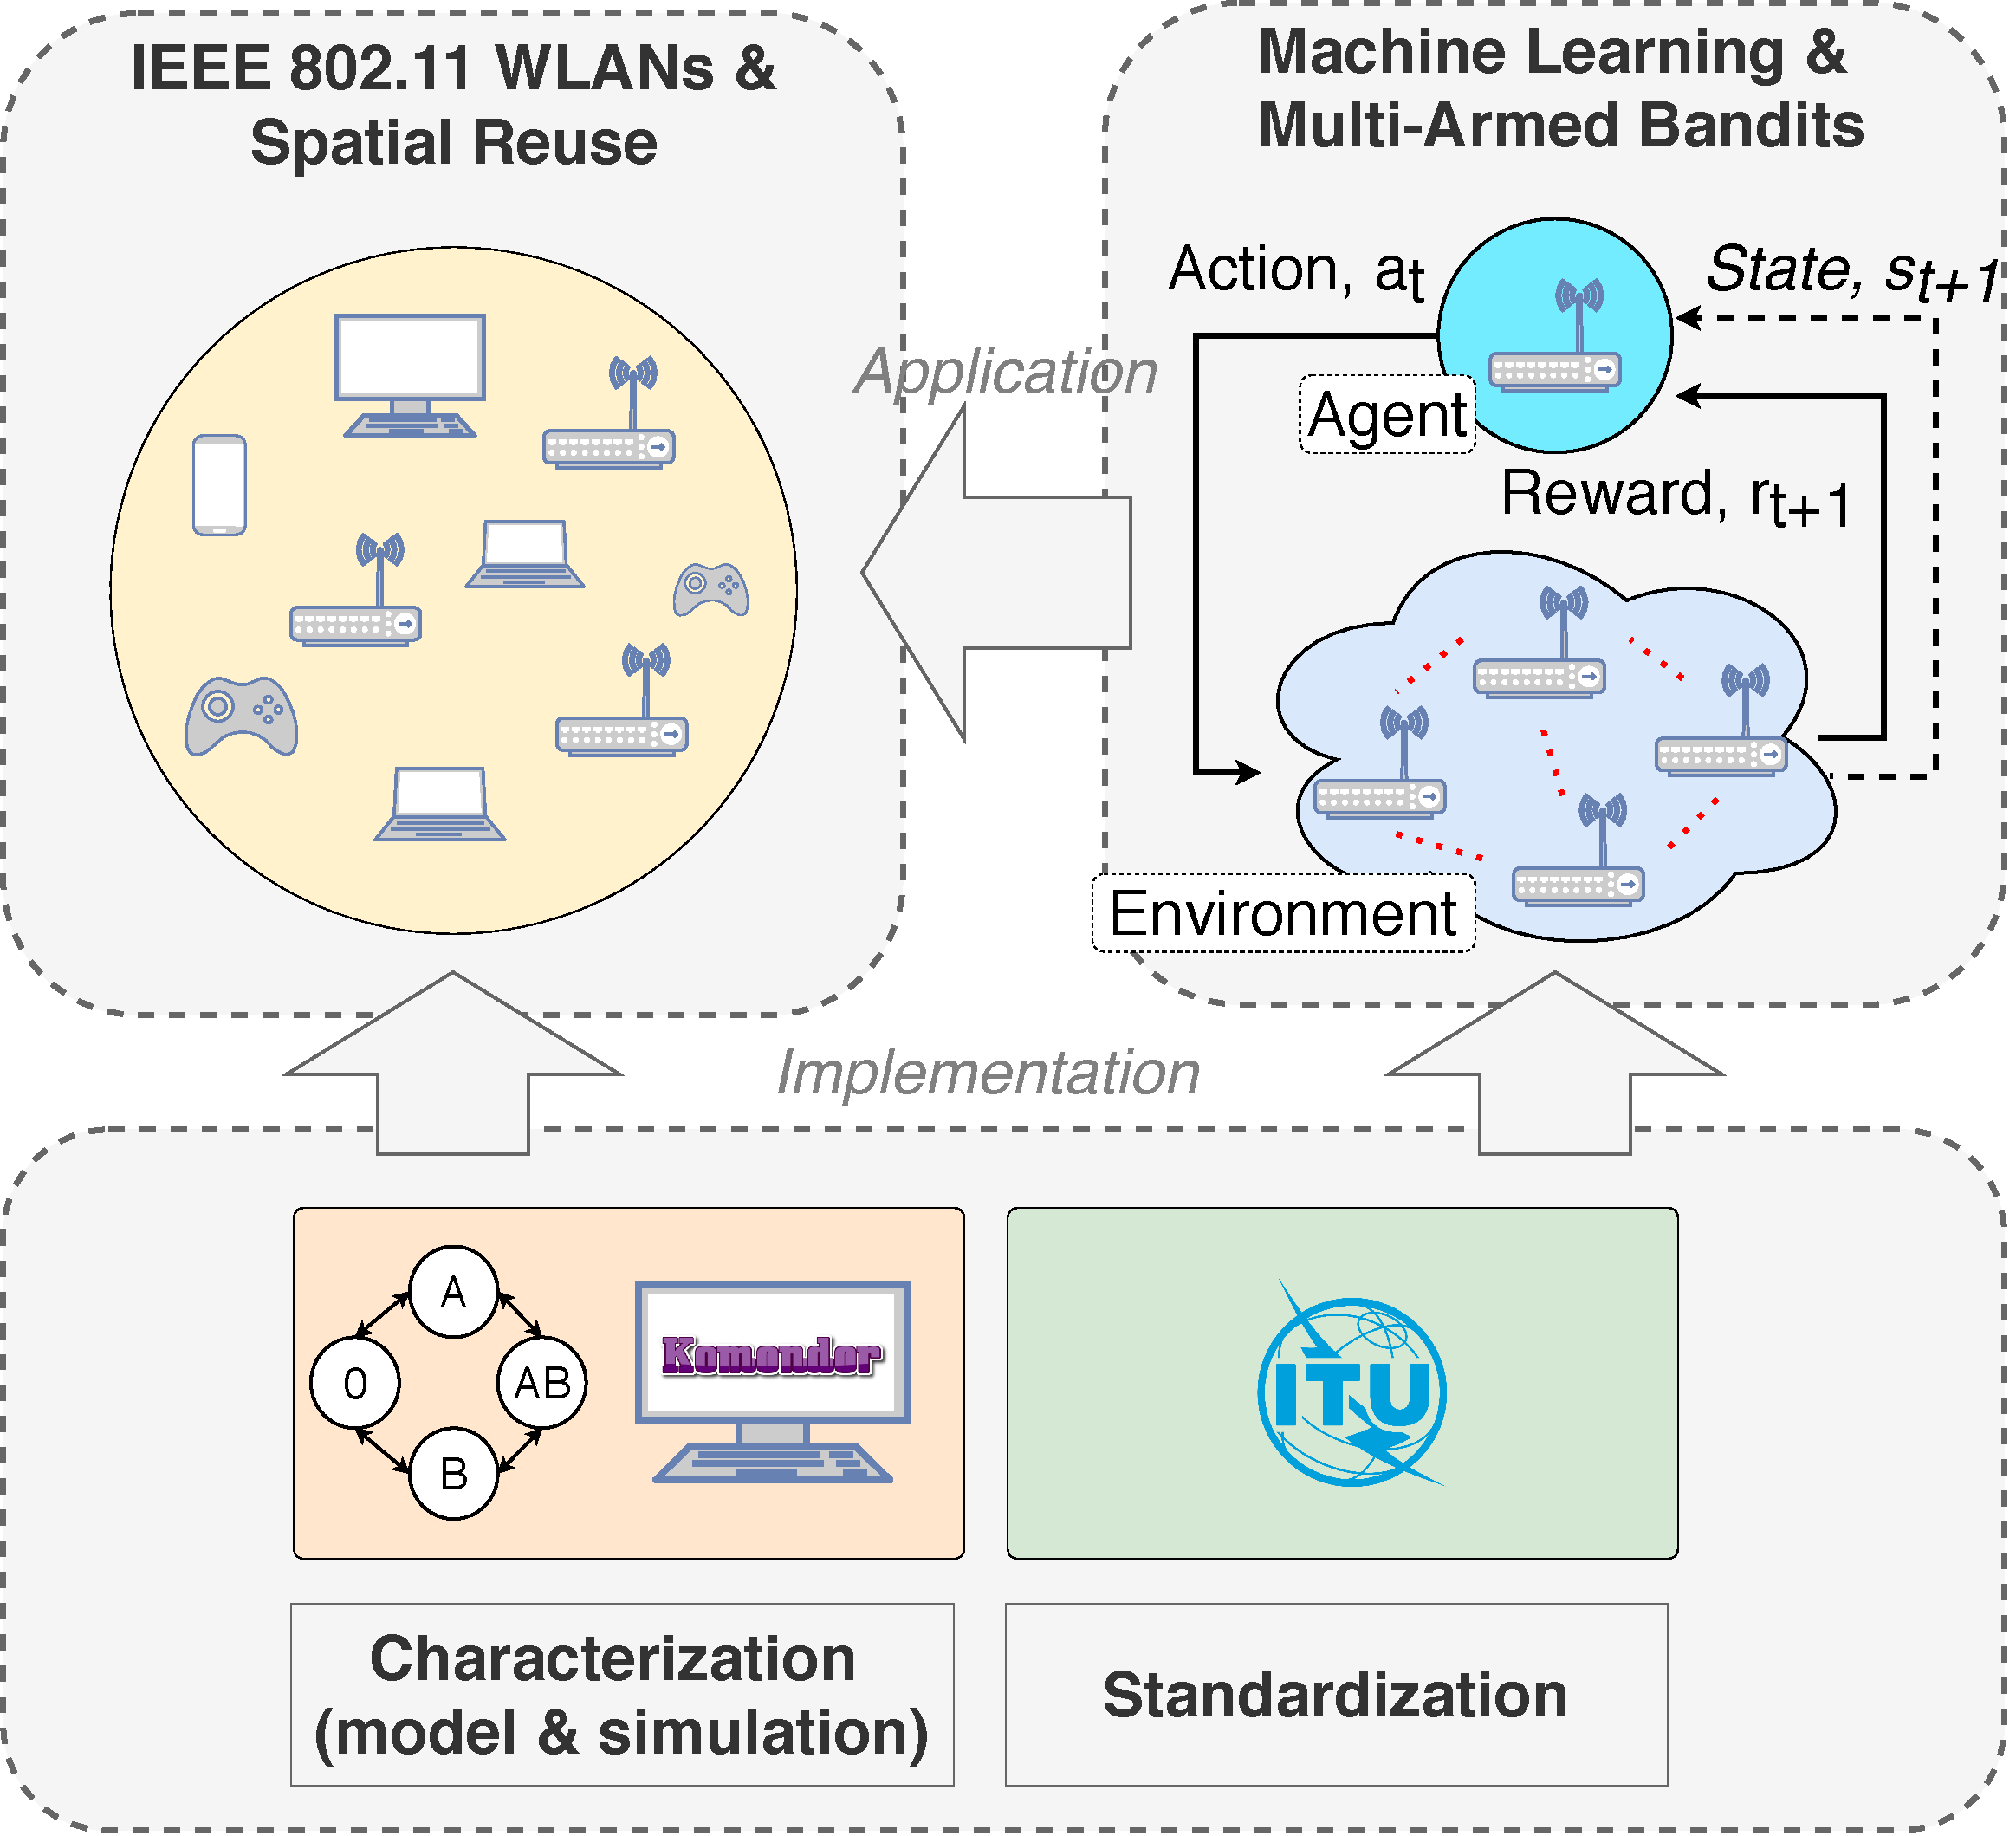
\includegraphics[width=.9\textwidth,keepaspectratio]{img/thesis_graphical_abstract}
		\end{figure}
	\end{column}
	\begin{column}{6cm}			
		\begin{enumerate}
			\item In-depth study of IEEE 802.11ax SR technology
			\begin{itemize}
				\item Tutorial
				\item Characterization and model 
				\item Performance evaluation
			\end{itemize}
			\pause
			\item Multi-player setting for SR
			\begin{itemize}
				\item Suitability in decentralized WLANs
				\item Study on performance gains in realistic scenarios
				%\item Pros/cons of selfish and collaborative goals
			\end{itemize}
			\pause
			\item Practical aspects for adopting ML in communications
			\begin{itemize}		
				\item Architectural considerations
				\item Reliability on AI/ML
			\end{itemize}
		\end{enumerate}
	\end{column}
\end{columns}

\end{frame}

\begin{frame}{Table of contents} % and our simple frame
	\tableofcontents
\end{frame}

%%%%%%%%%%%%%%
%%% Spatial Reuse
%%%%%%%%%%%%%%
\section{Spatial Reuse}

% Problem description
\subsection{}
\begin{frame}{Spatial Reuse in a nutshell}
		\pause
		\begin{block}{Methods to address density in wireless networks}
			\begin{itemize}
				\item \textbf{Time:} scheduling, medium access adaptation
				\item \textbf{Frequency:} Dynamic spectrum access, Dynamic channel bonding
				\item \textbf{Space:} Directional transmissions, Interference cancellation, \textit{Transmit power control}, \textit{Sensitivity adjustment}
			\end{itemize}
		\end{block}	
		\pause
		\begin{columns}
			\begin{column}{5.6cm}
				\begin{exampleblock}{Network's goals}
					\begin{itemize}
						\item Increase spectrum utilization
						\item Improve efficiency
						%\item Overcome inter-BSS interference
						\item More parallel transmissions
					\end{itemize}
				\end{exampleblock}	
			\end{column}
			\pause
			\begin{column}{5.6cm}
				\begin{alertblock}{User's goals}
					\begin{itemize}
						\item Increase transmission opportunities (TXOPs)
						\item Improve throughput
						\item Reduce delay
					\end{itemize}
				\end{alertblock}	
			\end{column}
		\end{columns}
\end{frame}

\subsection{}
\begin{frame}{Effects of tuning the transmit power}
\begin{figure}
	\animategraphics[loop,autoplay,width=\linewidth]{8}{img/anim1/anim-}{1}{77}
\end{figure}
\end{frame}

\subsection{}
\begin{frame}{Effects of tuning sensitivity}
\begin{figure}
	\animategraphics[loop,autoplay,width=\linewidth]{8}{img/anim2/anim-}{1}{77}
\end{figure}
\end{frame}

\subsection{}
\begin{frame}{Spatial reuse techniques in wireless networks}
\begin{figure}[ht!]
	\centering
	\resizebox{.9\textwidth}{!}{\begin{forest}
			forked edges,
			for tree={
				grow'=0,
				draw,
				align=c,
				font=\sffamily,
				rounded corners,
			},
			highlight/.style={
				thick,
				font=\sffamily\bfseries
			}
			[{Spatial Reuse\\Techniques}, highlight, fill=gray!30
			[{CS/CCA adaptation}, for tree={child, fill=green!30}
			[{Analysis: \cite{zhu2008optimal, jamil2014improving}},font=\fontsize{12}{0}\selectfont]
			[{Iterative methods: \cite{selinis2018control, ropitault2018evaluation}},font=\fontsize{12}{0}\selectfont]
			[{Pre-defined solutions: \cite{murakami2015improving, oni2015ap}},font=\fontsize{12}{0}\selectfont]
			[{Global solutions: \cite{nakahira2014centralized, afifi2016throughput}},font=\fontsize{12}{0}\selectfont]
			]
			[{Power control}, for tree={child, fill=yellow!20}
			[{Iterative methods: \cite{li2014energy,chevillat2005dynamic}},font=\fontsize{12}{0}\selectfont]
			[{Pre-defined solutions: \cite{chang2007power,tang2011improving}},font=\fontsize{12}{0}\selectfont]
			[{Global solutions: \cite{li2011achieving,tang2014joint}},font=\fontsize{12}{0}\selectfont]
			]
			[{Joint CS/CCA adaptation\\ \& Power control}, for tree={child, fill=cyan!30}
			[{Analysis: \cite{yamamoto2017analysis,iwata2019analysis}},font=\fontsize{12}{0}\selectfont]
			[{Iterative methods: \cite{jamil2015preserving,mhatre2007interference}},font=\fontsize{12}{0}\selectfont]
			[{Pre-defined solutions: \cite{jamil2015efficient,jamil2016novel}},font=\fontsize{12}{0}\selectfont]
			]
			]
	\end{forest}}
	\label{fig:sr_survey}
\end{figure}
\blfootnote{\scriptsize The set of referenced publications has been reduced for spacing purposes. The entire set of references can be found in the thesis document.}
\end{frame}

\subsection{}
\begin{frame}{Spatial reuse in IEEE 802.11ax}
\pause
\begin{itemize}
	%\item Baseline: DSC~\cite{smith2017dynamic}
	\item Two mechanisms: 
	\begin{enumerate}
		\item \textit{OBSS/PD-based SR} 
		\item \textit{Parametrized SR}
\end{enumerate}
	\item Common features: fast source identification, sensitivity adjustment, tx power limitation
\end{itemize}
\pause
\begin{columns}
	\begin{column}{6.5cm}
		\begin{figure}
			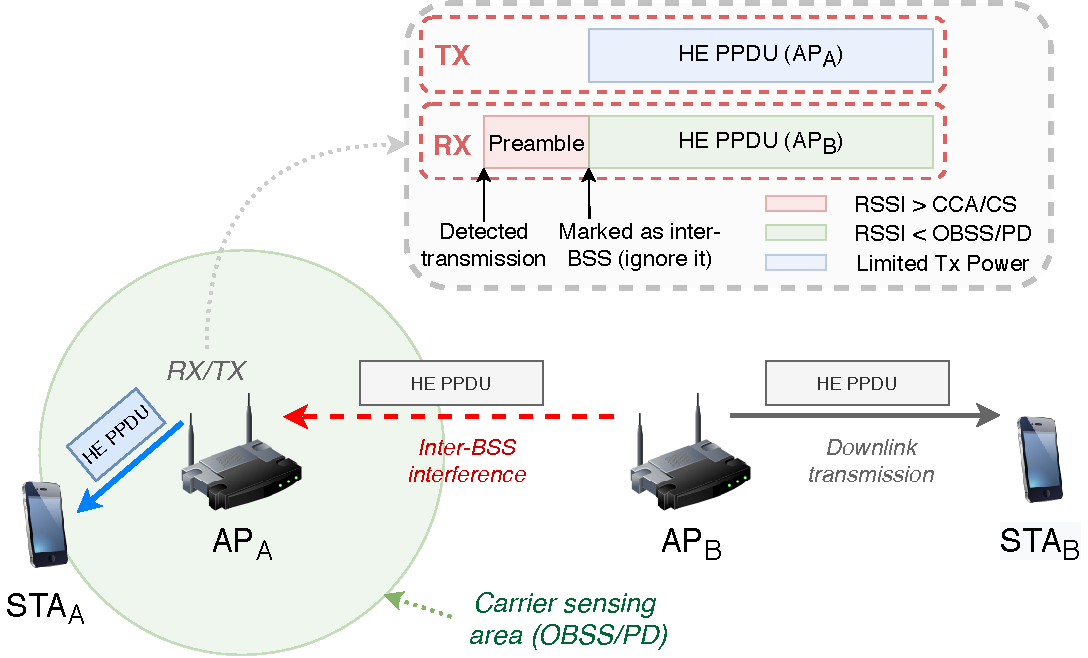
\includegraphics[width=.9\textwidth,height=\textheight,keepaspectratio]{img/example_obsspd_sr}
			%\caption{OBSS/PD-based SR}
		\end{figure}
	\end{column}
	\pause	
	\begin{column}{6cm}
		\begin{figure}
			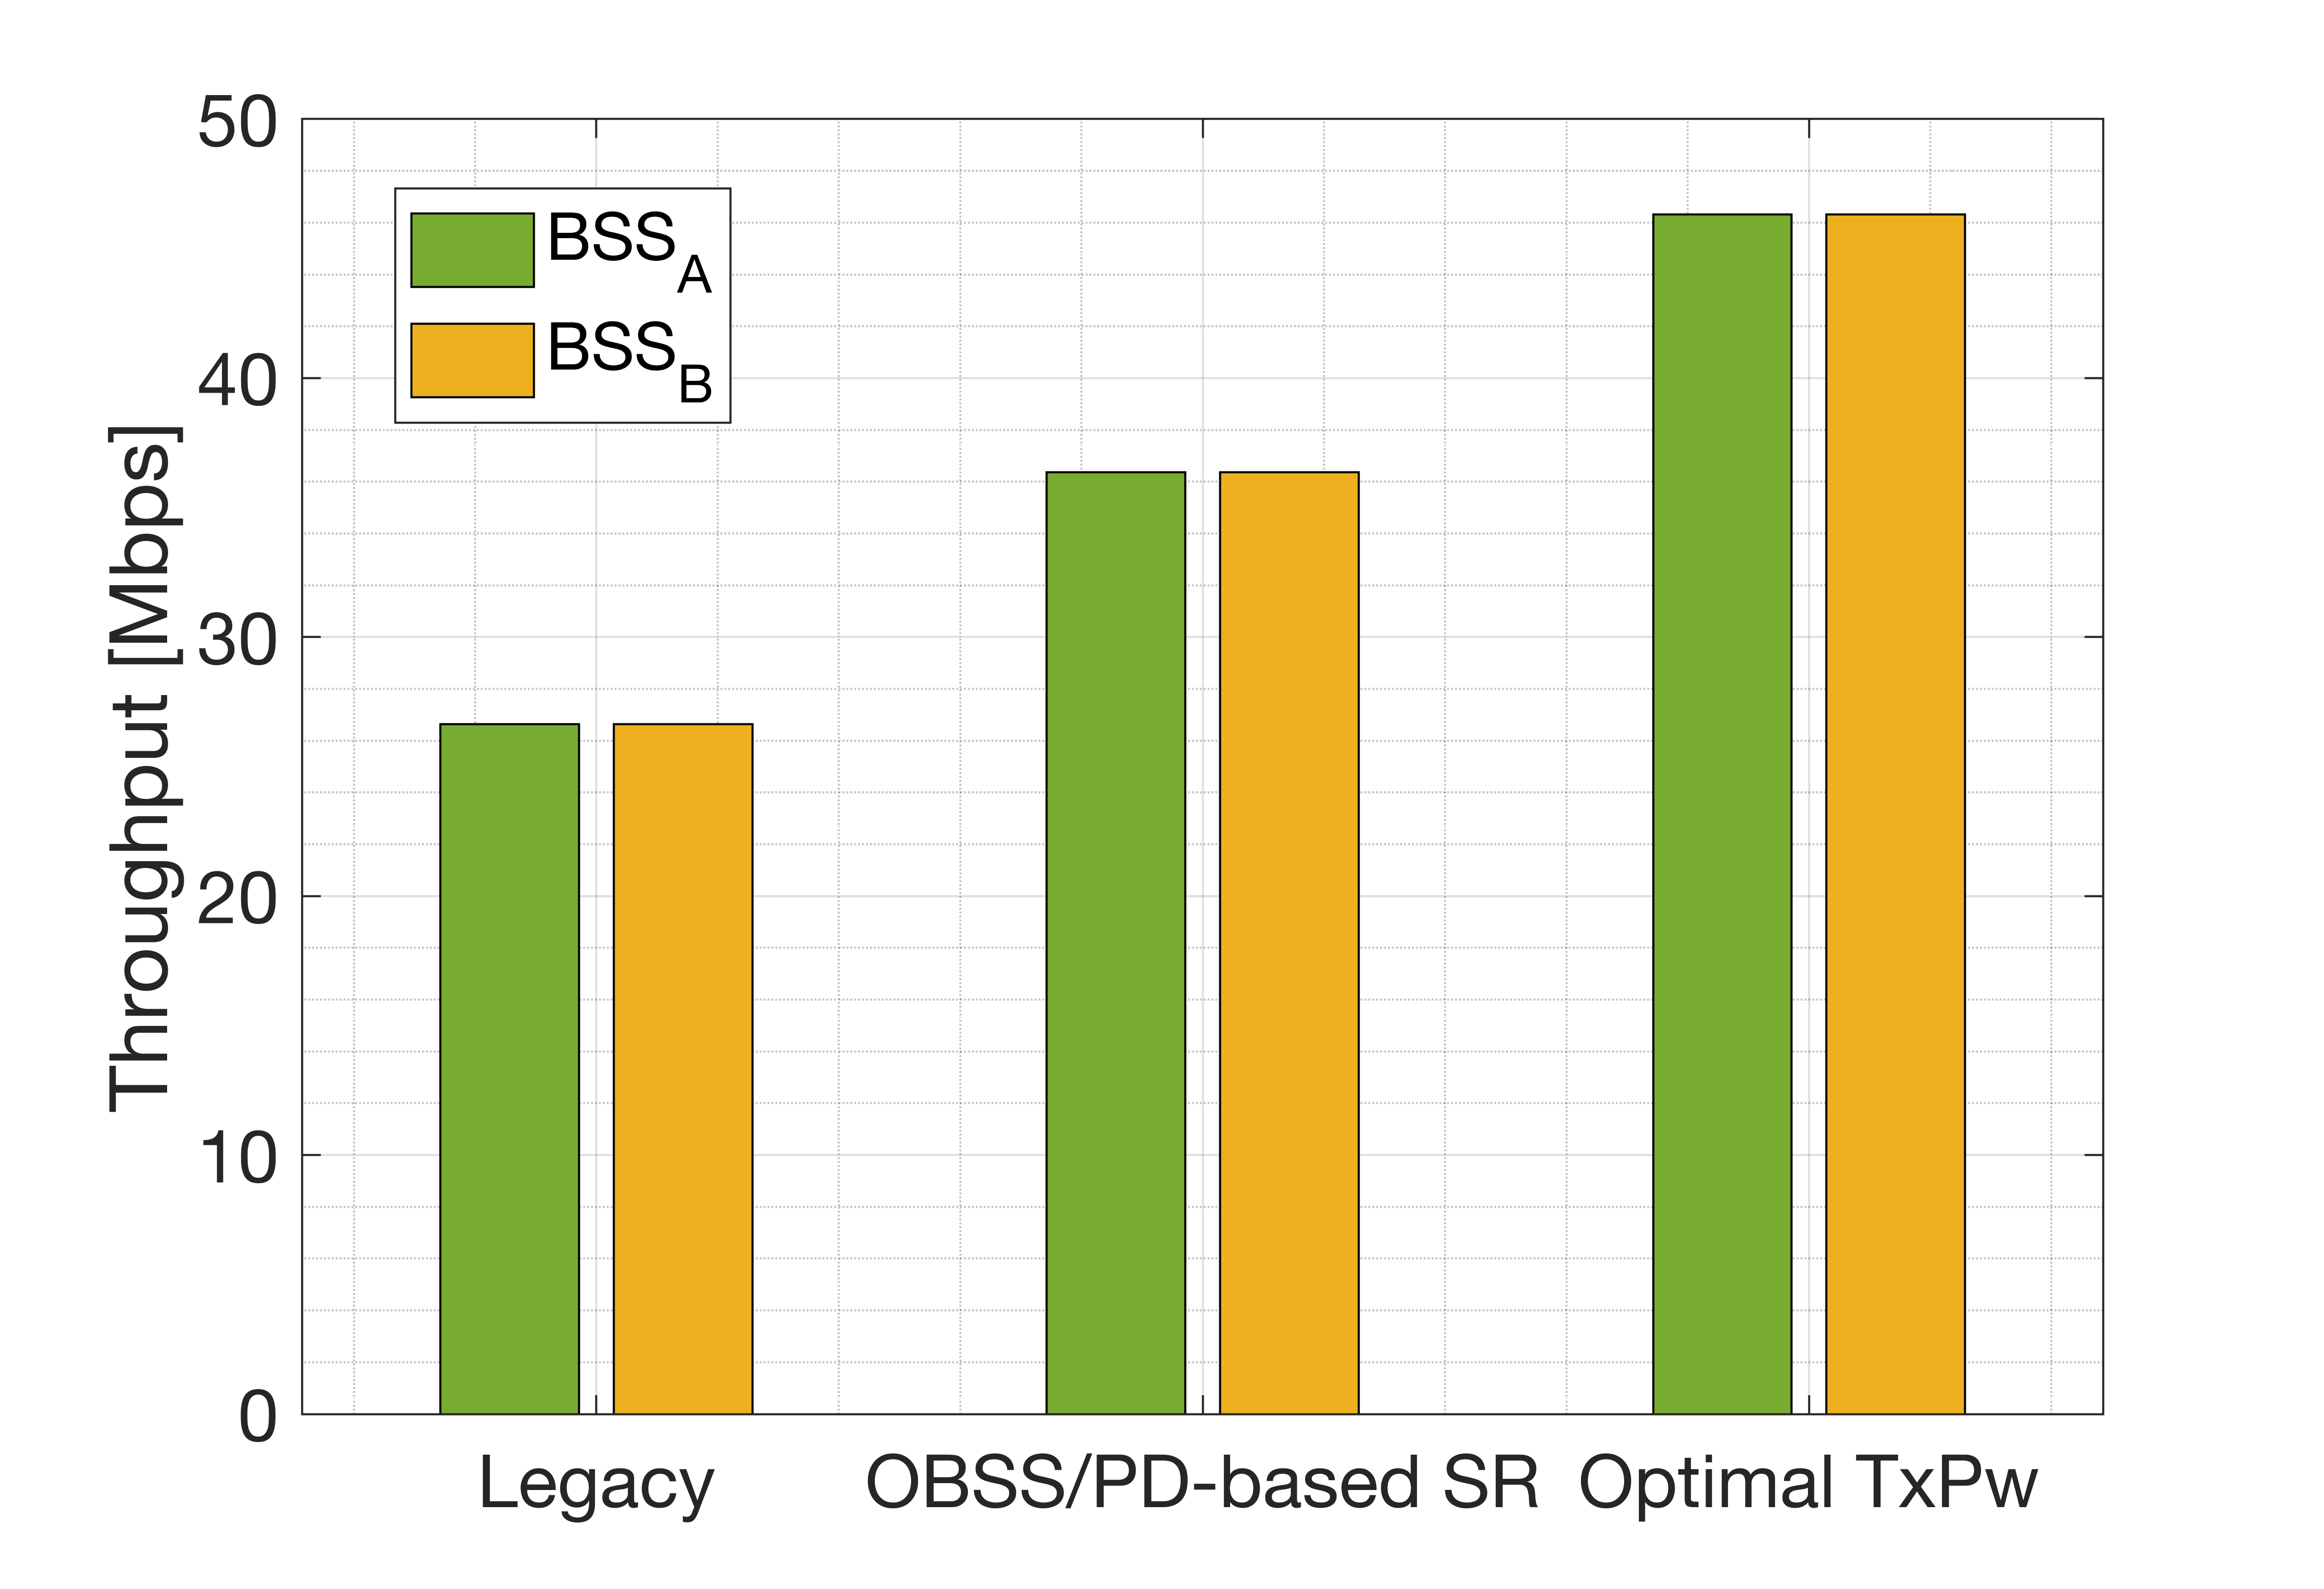
\includegraphics[width=.8\textwidth,height=\textheight,keepaspectratio]{img/thesis_sr_test}
		\end{figure}
		\vspace{-1cm}
		\begin{center}
			\begin{minipage}{5cm}
				\begin{alertblock}{}
				\centering
				\scriptsize Too conservative $\rightarrow$ Moderate gains
			\end{alertblock}
			\end{minipage}
		\end{center}
	\end{column}
\end{columns}

\end{frame}

\subsection{}
\begin{frame}{Spatial reuse in future IEEE 802.11 amendments}
\pause
	\begin{itemize}
		\item Multi-AP coordination \cite{csr}
		\item Exchange information and coordinate \textbf{simultaneous} Tx
		\item Two main proposals for IEEE 802.11be: 
		\begin{enumerate}
			\item \textbf{Coordinated SR (CSR)}
			\item PSR with beamforming/null steering
		\end{enumerate}
	\end{itemize}
\pause
	\begin{figure}
		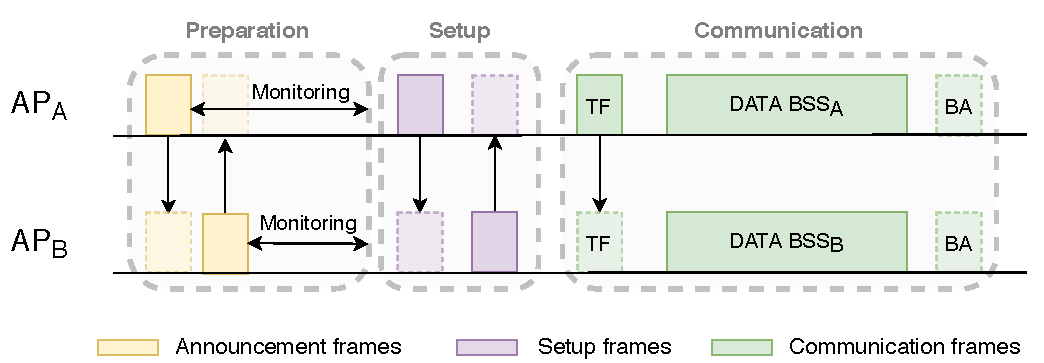
\includegraphics[width=.65\textwidth,keepaspectratio]{img/coordinated_sr}
		%\caption{Coordinated SR}
	\end{figure}
	\vspace{-.8cm}

	\pause

	\begin{center}
		\begin{minipage}{11cm}
			\begin{alertblock}{}
				\centering
				\textbf{Open discussion points:} extension to UL, measurement phase, role of OFDMA, optimization goals...
			\end{alertblock}
		\end{minipage}
	\end{center}

\end{frame}

%%%%%%%%%%%%%%
%%% Machine Learning
%%%%%%%%%%%%%%
\section[ML in Communications]{Machine Learning for Spatial Reuse}

\subsection{}
\begin{frame}{The emergence of AI for communications}
\vspace{-0.25cm}
\begin{columns}
	\begin{column}{5.5cm}
		\pause
		\begin{block}{Model-based}
			\begin{itemize}
				\item Hand-crafted solution %(theoretical considerations and/or measurements)
				\item Accuracy vs tractability
				\item Generalization				 
			\end{itemize}
		    \vspace{-.5cm}
			\begin{figure}
				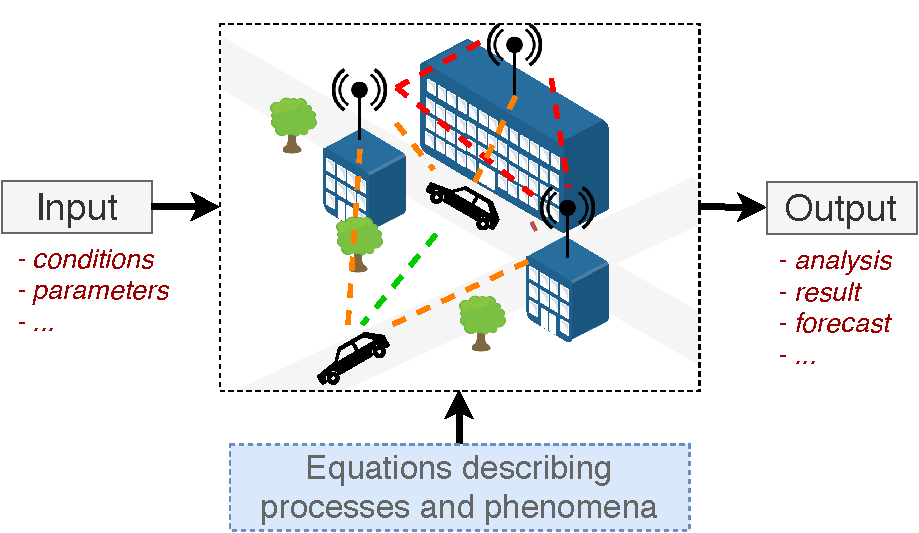
\includegraphics[width=.9\textwidth,keepaspectratio]{img/modelbased}
			\end{figure}
		\end{block}	
	\end{column}
	\begin{column}{5.5cm}
		\pause
		\begin{exampleblock}{Data-driven}
			\begin{itemize}
				\item Learn from data
				\item Address complexity
				\item Adaptability
			\end{itemize}
			\vspace{-.5cm}
			\begin{figure}
				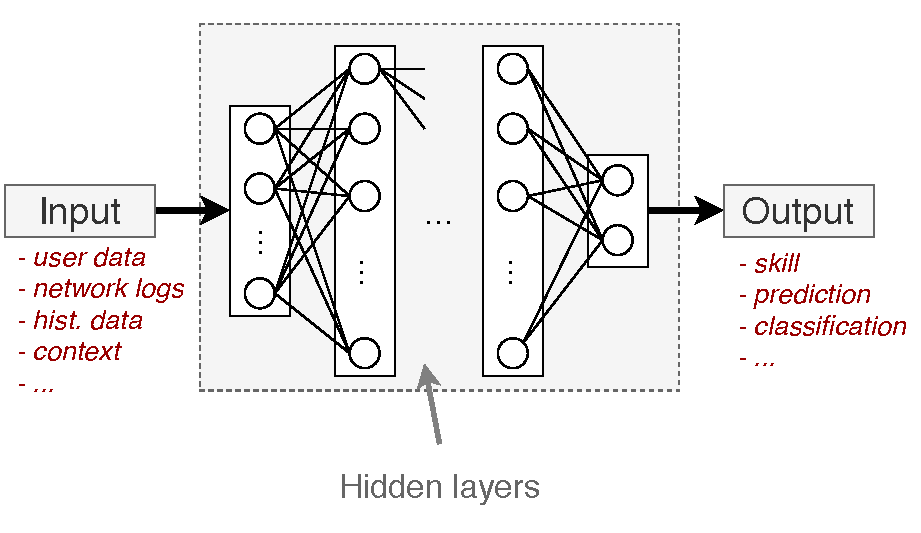
\includegraphics[width=.9\textwidth,keepaspectratio]{img/datadriven}
			\end{figure}
		\end{exampleblock}	
	\end{column}
\end{columns}
\pause
\vspace{-0.25cm}
\begin{center}
	\begin{minipage}{9cm}
		\begin{alertblock}{}
			\centering
			\textbf{Enablers} for adoption:
			\begin{itemize}	
				\item Infrastructure (architecture, capacity, data)
				\item Reliability and trustworthiness
			\end{itemize}
		\end{alertblock}
	\end{minipage}
\end{center}

\end{frame}

\subsection{}
\begin{frame}{Machine-learning-aware communications}
\begin{columns}
	\begin{column}{6cm}
		\begin{figure}
			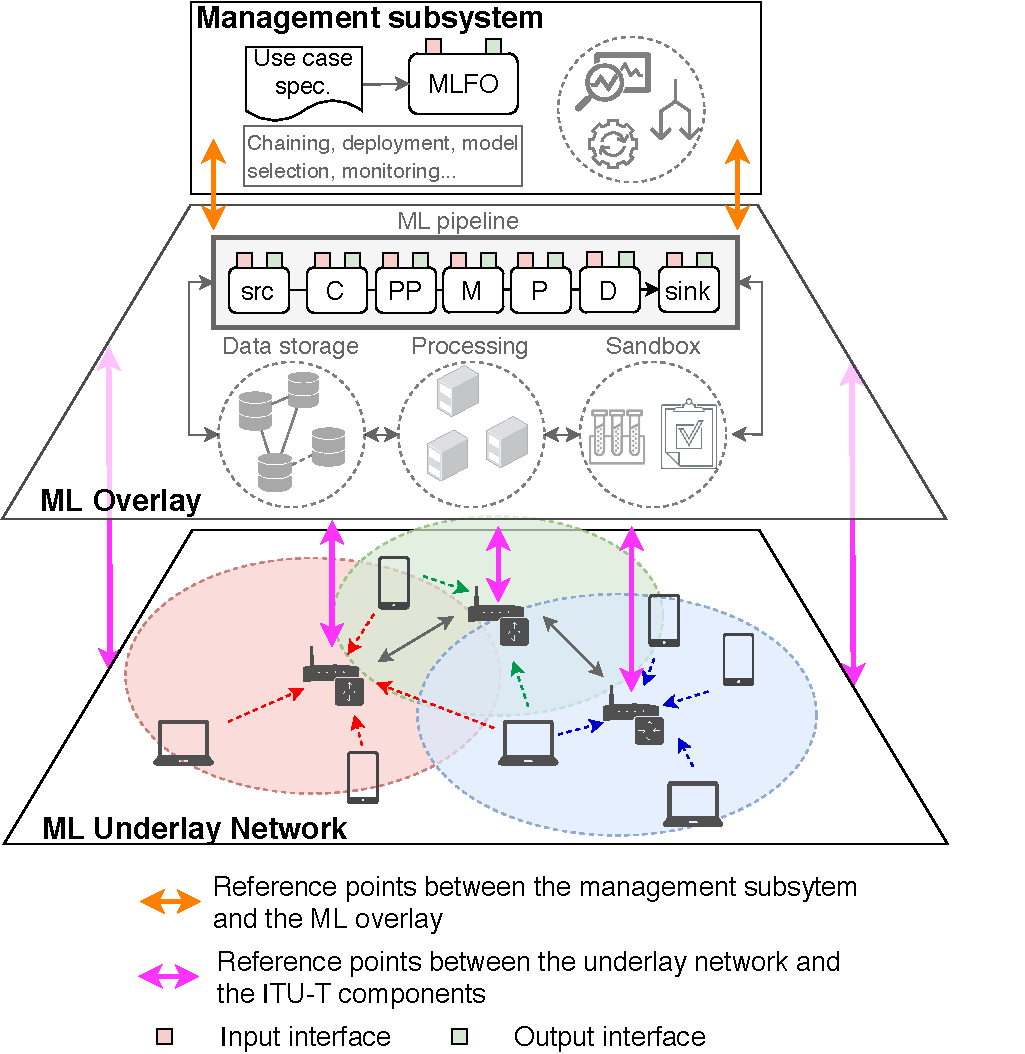
\includegraphics[width=.9\textwidth,height=\textheight,keepaspectratio]{img/itu_architecutre}
			%\caption{ITU-T ML-aware arch.}
		\end{figure}
	\end{column}
	\begin{column}{6cm}
		\pause
		\begin{block}{Architectural aspects}
			\begin{itemize}
				\item Framework in ITU-T Y.3172 recommendation \cite{y3172}
				\item Flexibility required for decentralized WLANs
			\end{itemize}
		\end{block}
		\pause
		\begin{exampleblock}{Reliability \& Trustworthiness}
			\begin{itemize}
				\item ML Sandbox
				\item \textbf{Test}, \textbf{train}, and \textbf{evaluate} ML models
				\item Simulators in closed-loop ML-based optimization
			\end{itemize}
		\end{exampleblock}
	\end{column}
\end{columns}
\end{frame}

\subsection{}
\begin{frame}{Multi-agent systems}

\begin{columns}
		\begin{column}{5.5cm}
		\begin{figure}
			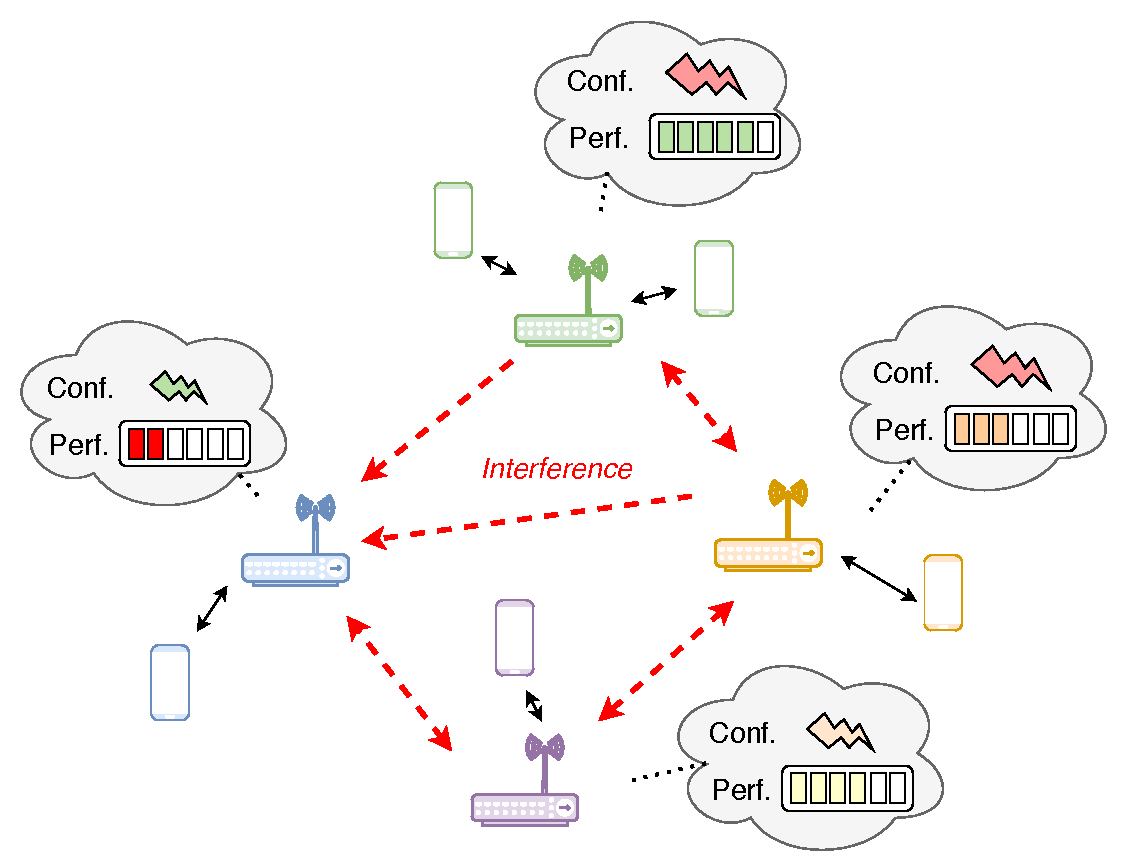
\includegraphics[width=.95\textwidth,keepaspectratio]{img/multi_agent}
			%\caption{Multi-agent WLAN}
		\end{figure}
	\end{column}
	\pause
	\begin{column}{6cm}
		\begin{block}{Motivation}
			\begin{itemize}	
				\item Distributed nature of WLANs
				\item Complexity of SR
				%			\begin{itemize}
				%				\item High-density
				%				\item Interactions among devices
				%				\item Combinatorial number of configurations
				%			\end{itemize}
				\item Split a big problem into sub-problems
			\end{itemize}
		\end{block}
		\pause
		\begin{alertblock}{Considerations}
			\begin{itemize}	
				\item Conflicting requirements% (Competition vs Cooperation)
				\item Non-stationarity / Equilibrium
				\item Suboptimal performance
				\item Nexus with Game Theory
			\end{itemize}
		\end{alertblock}
	\end{column}
\end{columns}

\end{frame}

\subsection{}
\begin{frame}{Multi-Armed Bandits for SR}
\vspace{-0.65cm}
\begin{columns}
	\begin{column}{6cm}
		\begin{figure}
			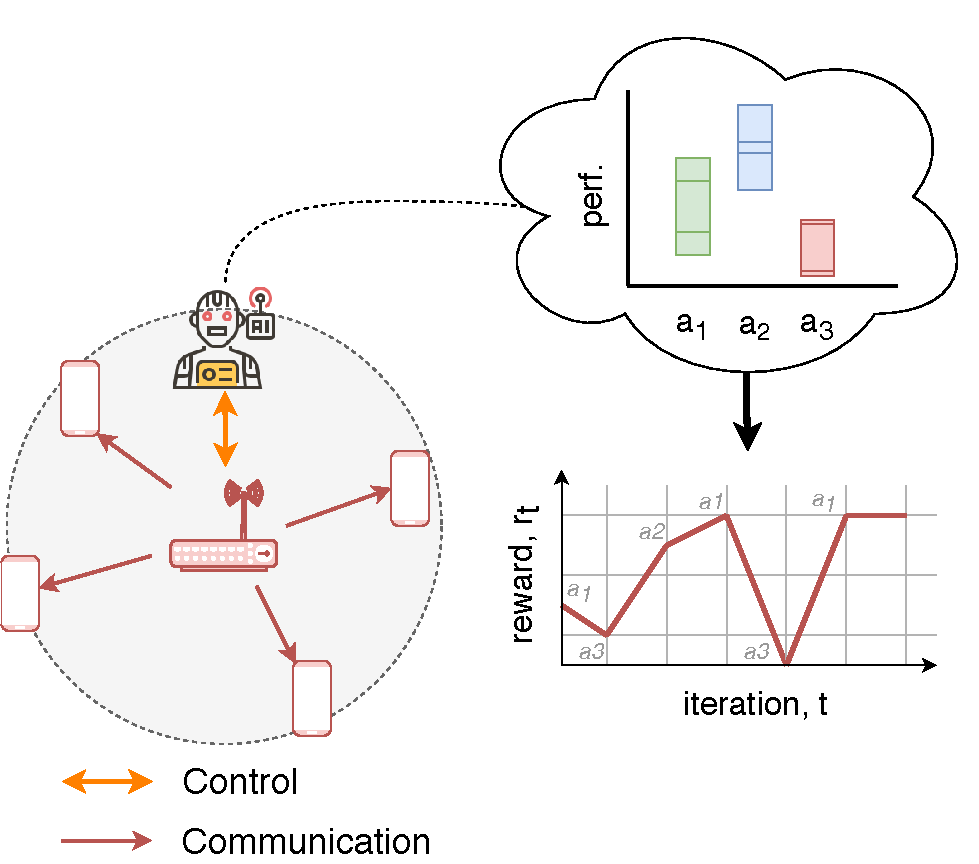
\includegraphics[width=.75\textwidth,height=\textheight,keepaspectratio]{img/agent_sr}
			%\caption{Agent's operation}
		\end{figure}
	\vspace{-0.75cm}
	\pause
		\begin{figure}
			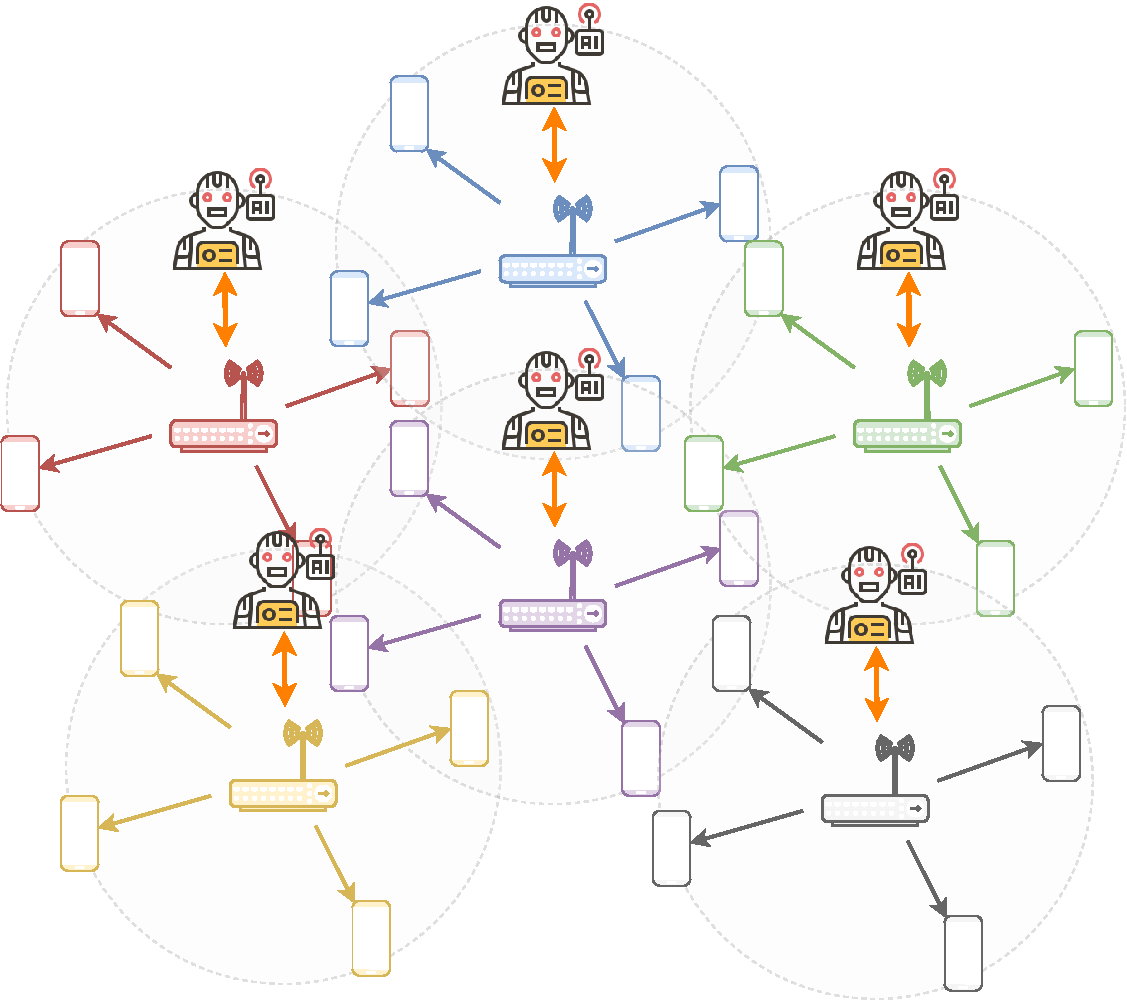
\includegraphics[width=.6\textwidth,height=\textheight,keepaspectratio]{img/multi_agent_sr}
			%\caption{Agent's operation}
		\end{figure}
	\end{column}
	\pause
	\begin{column}{5.5cm}
		\begin{block}{Suitability}
			\begin{itemize}
				\item Bandit feedback % information of other actions is not revealed
				\item Statistical characteristics
				\item Non-stationarity % trade-off learnings and dynamicity of the environment
				\item Fast improvements
			\end{itemize}
		\end{block}
		\pause
		\begin{exampleblock}{Contribution}
			\begin{itemize}
				\item Analysis: performance, convergence, adaptability
				\item Local vs shared information
				\item Algorithms: $\varepsilon$-greedy, UCB, EXP3, Thompson sampling
			\end{itemize}
		\end{exampleblock}
	\end{column}
\end{columns}
\end{frame}

\subsection{}
\begin{frame}{MAB-based applications for communications}
\begin{table}[]
	%\caption{Overview of bandit-based applications for communications}
	\label{tab:mabs_communications}
	\resizebox{\textwidth}{!}{%
		\begin{tabular}{|l|l|l|l|l|}
			\hline
			\multicolumn{1}{|c|}{\textbf{Problem}} & \multicolumn{1}{c|}{\textbf{Modeling}} & \multicolumn{1}{c|}{\textbf{Goals}} & \multicolumn{1}{c|}{\textbf{\begin{tabular}[c]{@{}c@{}}Baseline algorithms\end{tabular}}} & \multicolumn{1}{c|}{\textbf{References}} \\ \hline
			\begin{tabular}[c]{@{}l@{}}Spectrum access \& \\ Channel selection\end{tabular} & \begin{tabular}[c]{@{}l@{}}Stochastic, non-stochastic, \\ restless, contextual, Markovian\\ bandits\end{tabular} & \begin{tabular}[c]{@{}l@{}}Decentralized optimal allocation, \\ optimize number of secondary\\ transmissions, $\epsilon$-correct ranking\end{tabular} & \begin{tabular}[c]{@{}l@{}}UCB, $\epsilon$-greedy,\\ calibrated forecasting\end{tabular} & \cite{anandkumar2011distributed,maghsudi2015channel} \\ \hline
			Power control & Non-stochastic bandits & Optimize SINR & \begin{tabular}[c]{@{}l@{}}Follow the perturbed leader,\\ exponential weighted average\end{tabular} & \cite{maghsudi2014joint} \\ \hline
			User association & \begin{tabular}[c]{@{}l@{}}Sleeping, Bernoulli,\\ non-stochastic bandits\end{tabular} & Energy saving, improve the throughput & UCB, $\epsilon$-greedy & \cite{maghsudi2017distributed,carrascosa2020multi} \\ \hline
			Inter-cell coordination & \begin{tabular}[c]{@{}l@{}}Adversarial, stochastic,\\ non-stochastic,\\ contextual bandits\end{tabular} & \begin{tabular}[c]{@{}l@{}}Optimize inter-cell frequency resources,\\ energy saving, map SON configurations \\ and operator objectives\end{tabular} & EXP3, UCB, $\epsilon$-greedy & \cite{coucheney2015multi, daher2017cognitive} \\ \hline
			Dynamic rate selection & Structured, Markovian bandits & \begin{tabular}[c]{@{}l@{}}Maximize the number of packets \\ successfully transmitted, \\ learn changes in the channel\end{tabular} & UCB & \cite{combes2014dynamic, zhao2020non} \\ \hline
			LTE/Wi-Fi coexistence & Convex bandits & Fair channel sharing & Online gradient descent & \cite{cano2018wireless} \\ \hline
		\end{tabular}%
	}
\end{table}
\pause
\begin{center}
	\begin{minipage}{8cm}
	\begin{alertblock}{}
		\centering
		Typically, the results in the literature lack of applicability in realistic scenarios
	\end{alertblock}
	\end{minipage}
\end{center}

\blfootnote{\scriptsize The set of referenced publications has been reduced for spacing purposes. The entire set of references can be found in the thesis document.}

\end{frame}

%%%%%%%%%%%%%%
%%% Methodology
%%%%%%%%%%%%%%
\section[Method. \& Enablers]{Methodology and Enablers}

\subsection{}
\begin{frame}{Model and analysis of SR}
\pause
	\begin{exampleblock}{Importance of models}
		\begin{itemize}
			\item Represent phenomena in wireless communications %(abstraction of essential features)
			\item Useful to understand particular technologies
%			\item Baseline: Bianchi \cite{bianchi2000performance}, SINR-based models \cite{guo2003spatial}, Stochastic geometry \cite{zhao2016stochastic}
%			\item Drawbacks: Unaffordable assumptions, focus on the PHY only
		\end{itemize}
	\end{exampleblock}
\pause
	\begin{block}{Related work for modeling SR}
		\begin{itemize}
			%\item Representation of protocols and phenomena in wireless communications (abstract essential features of a particular phenomena)
			\item \textbf{Baseline:} Bianchi \cite{bianchi2000performance}, SINR-based models \cite{guo2003spatial}, Stochastic geometry \cite{zhao2016stochastic}
			\item \textbf{Drawbacks:} assumptions, focus on the PHY or MAC only
		\end{itemize}
	\end{block}
\pause
	\begin{alertblock}{Continuous Time Markov Networks (CTMNs)}
		\begin{itemize}
			%\item In-between theory and simulation
			\item Additive interference \cite{barrachina2019dynamic} % Essential to represent SR (models for the MAC do not typically consider this, and models for the PHY do not capture MAC interactions)
			\item Implementation of OBSS/PD-based SR
			\item Validate SR and understand it in toy scenarios % Some assumptions (e.g., continuous backoff) and Computational cost
		\end{itemize}
	\end{alertblock}
\end{frame}

\subsection{}
\begin{frame}{Continuous Time Markov Networks (I)}
	\begin{figure}
		%\animategraphics[loop,autoplay,width=\linewidth]{0.25}{img/anim3/frame-}{1}{5}
		\only<1>{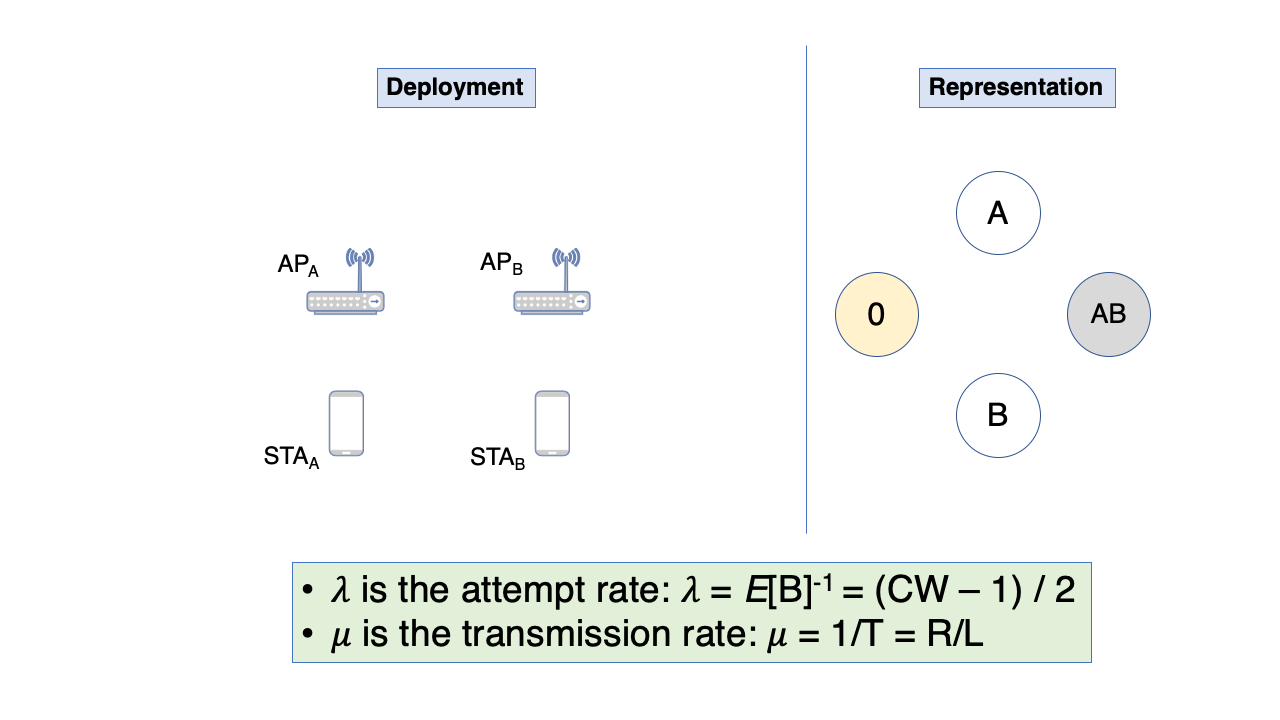
\includegraphics[width=\textwidth,height=\textheight,keepaspectratio]{img/anim3/frame-1}}
		\only<2>{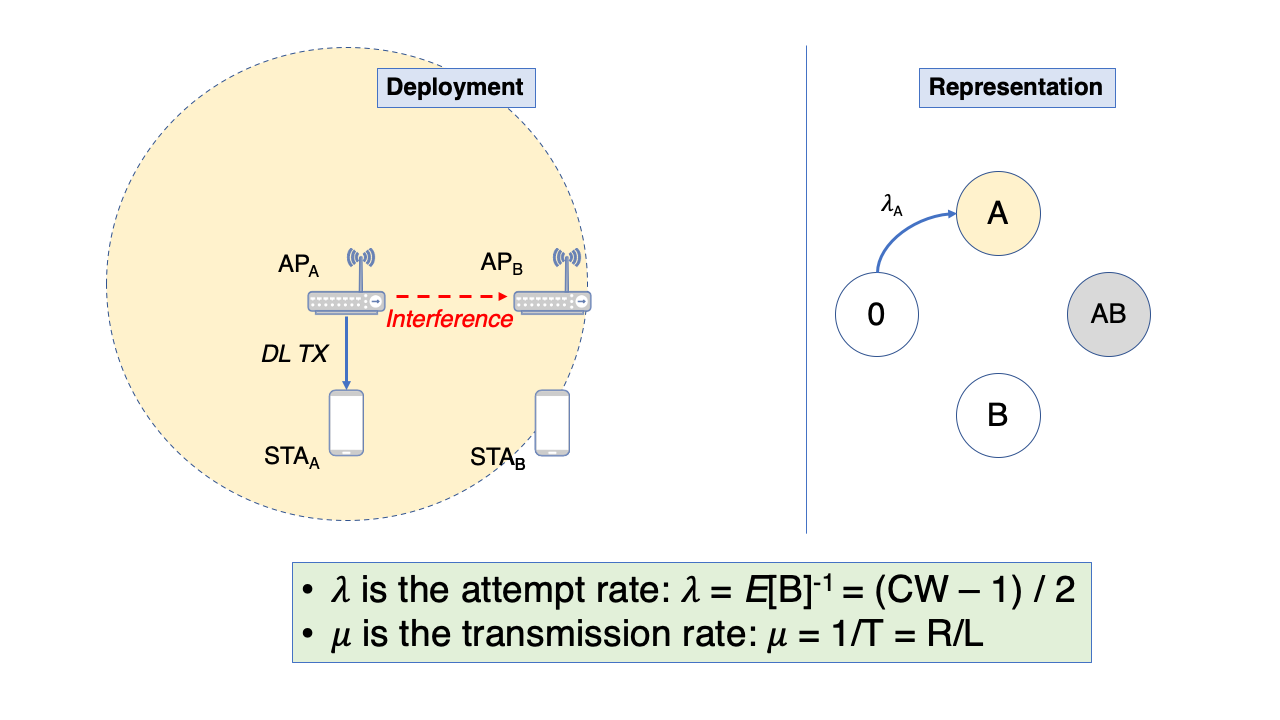
\includegraphics[width=\textwidth,height=\textheight,keepaspectratio]{img/anim3/frame-2}}
		\only<3>{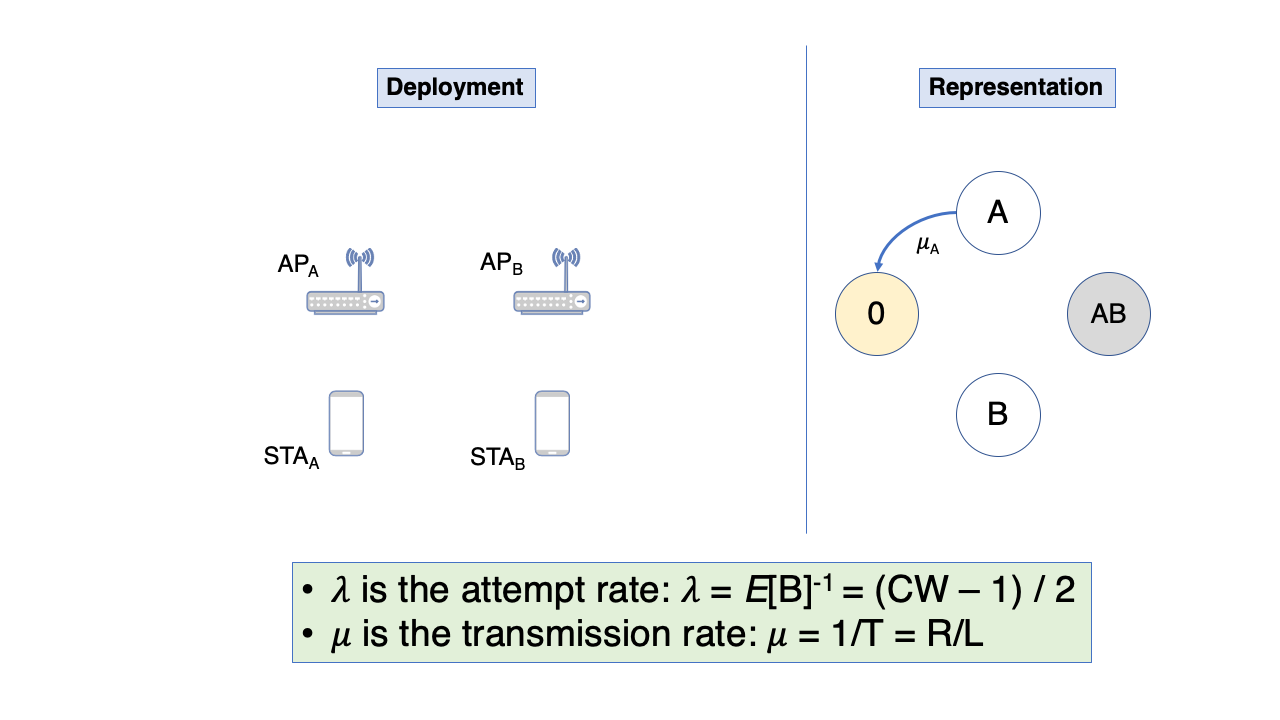
\includegraphics[width=\textwidth,height=\textheight,keepaspectratio]{img/anim3/frame-3}}
		\only<4>{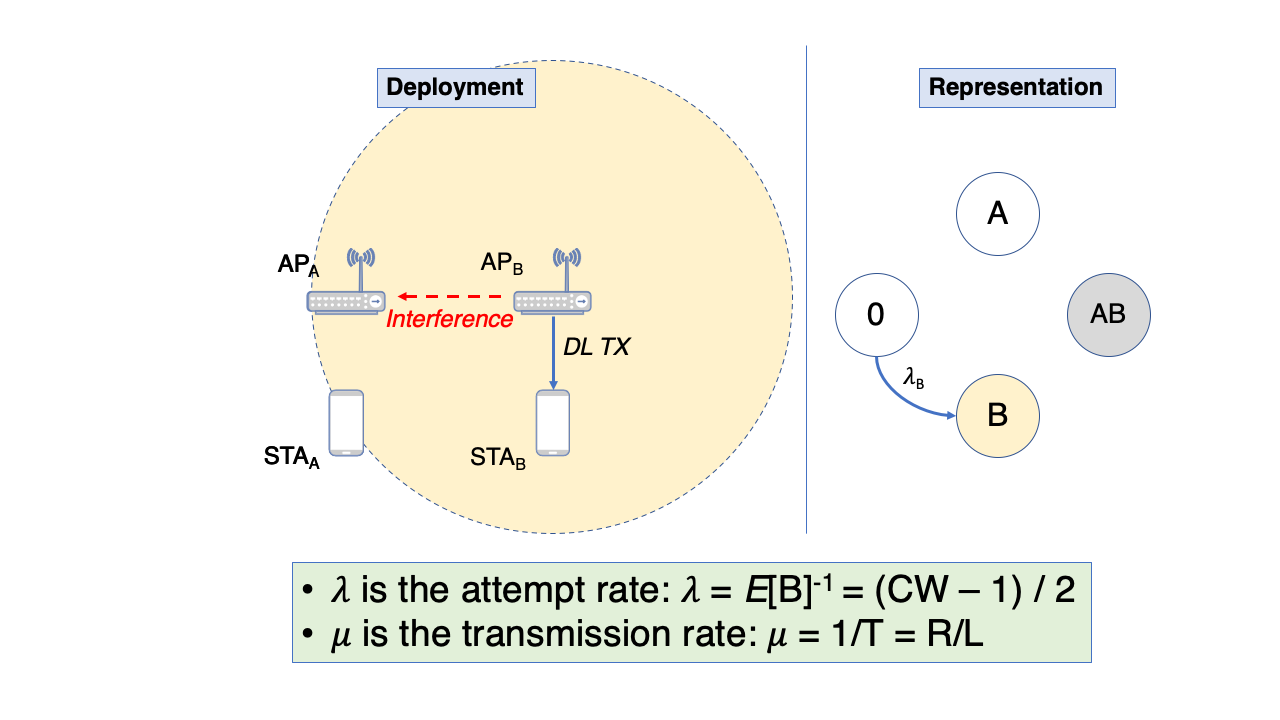
\includegraphics[width=\textwidth,height=\textheight,keepaspectratio]{img/anim3/frame-4}}
		\only<5>{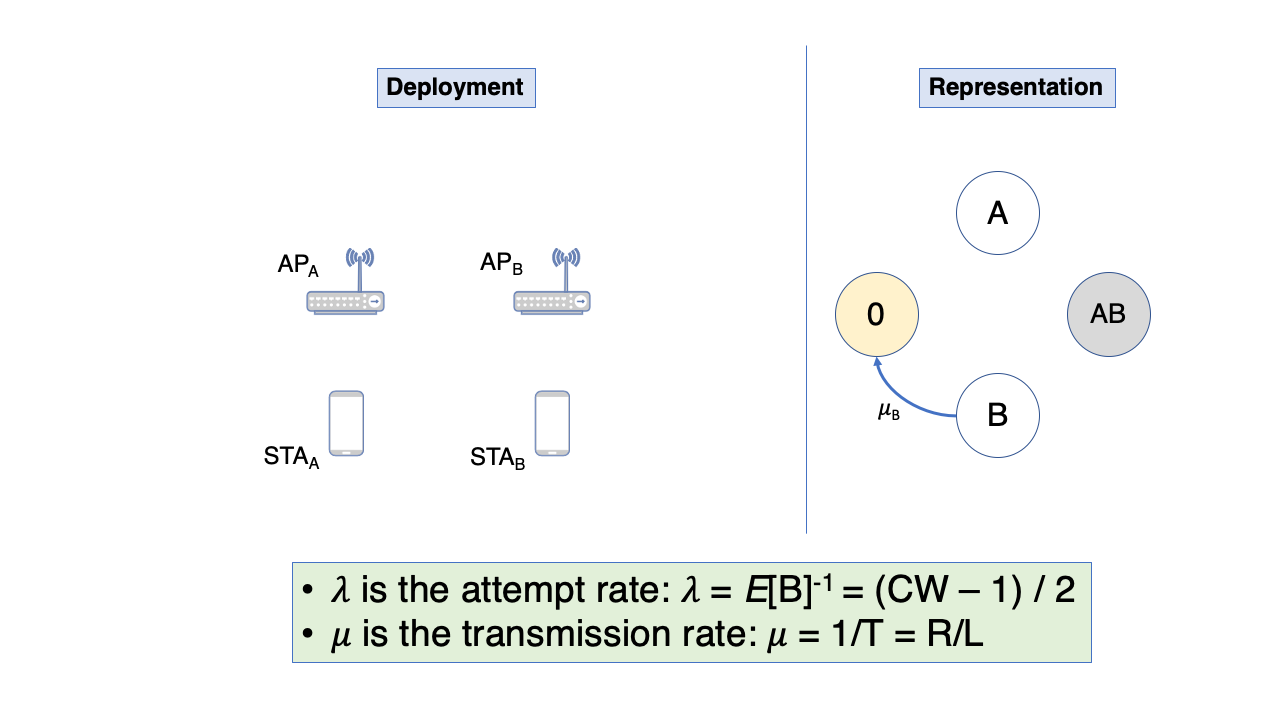
\includegraphics[width=\textwidth,height=\textheight,keepaspectratio]{img/anim3/frame-5}}
	\end{figure}
\end{frame}

\subsection{}
\begin{frame}{Continuous Time Markov Networks (II)}
\begin{figure}
	%\animategraphics[loop,autoplay,width=\linewidth]{0.25}{img/anim4/frame-}{1}{7}
	\only<1>{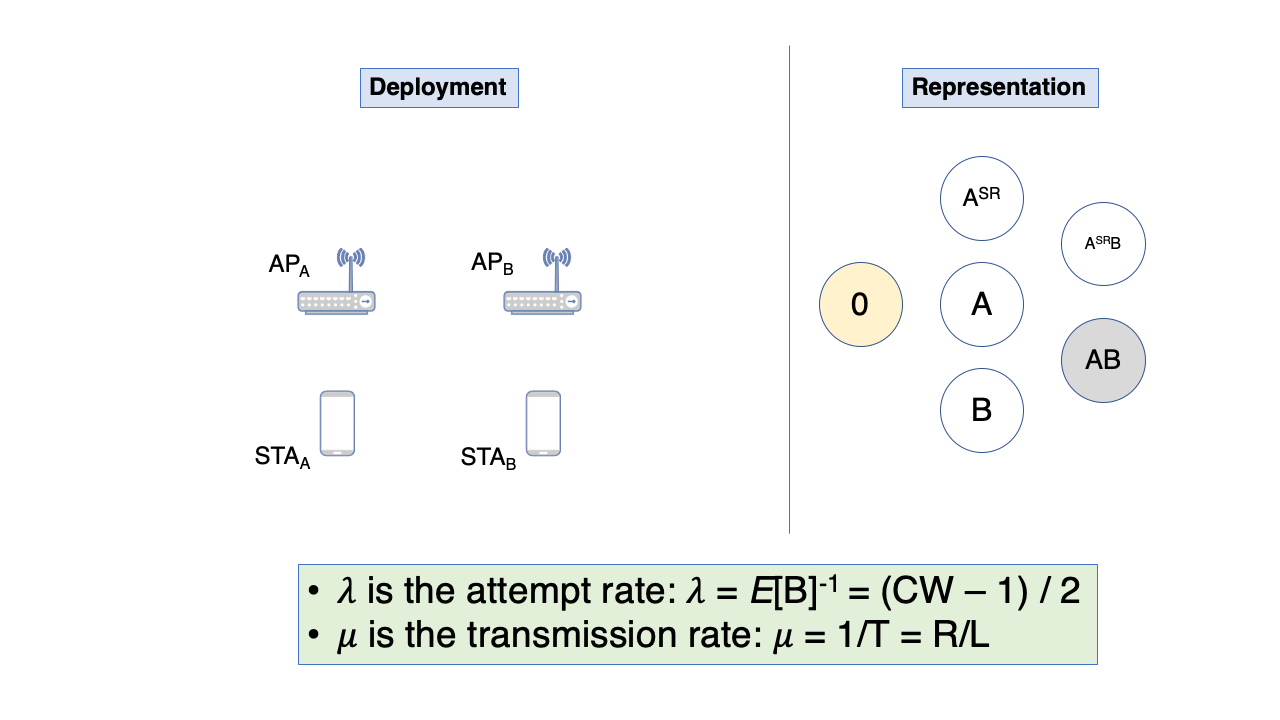
\includegraphics[width=\textwidth,height=\textheight,keepaspectratio]{img/anim4/frame-1}}
	\only<2>{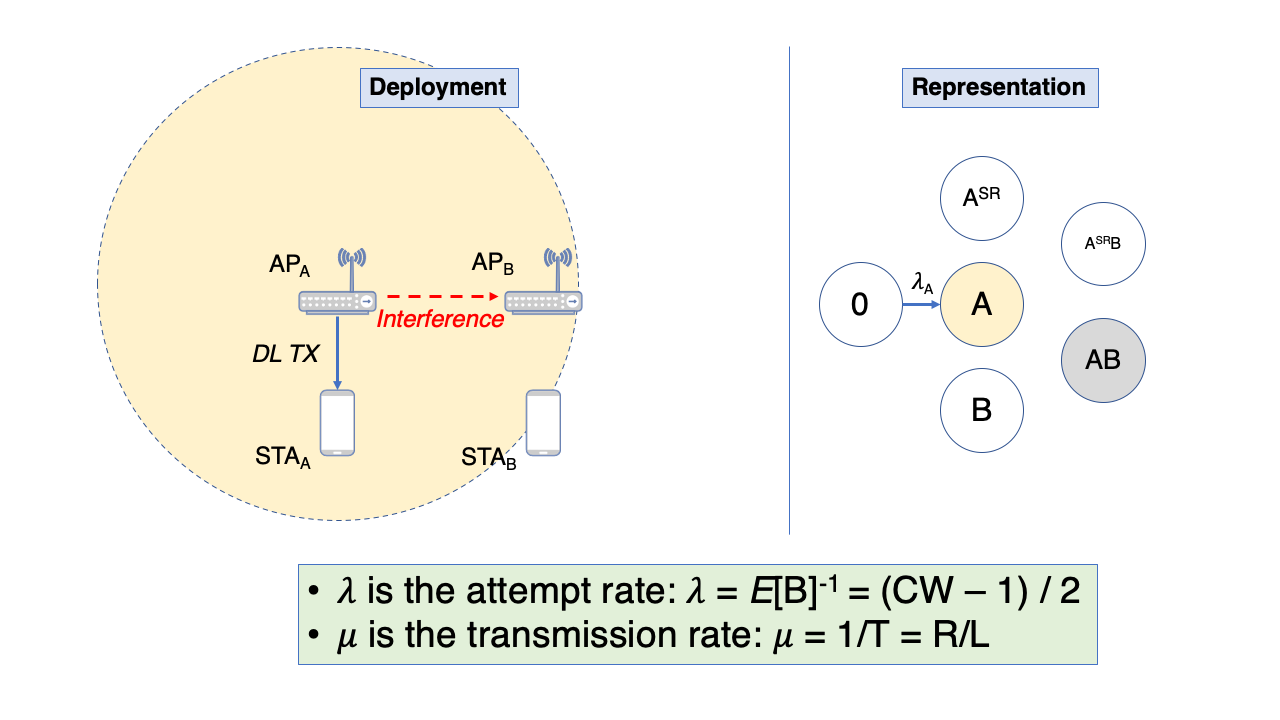
\includegraphics[width=\textwidth,height=\textheight,keepaspectratio]{img/anim4/frame-2}}
	\only<3>{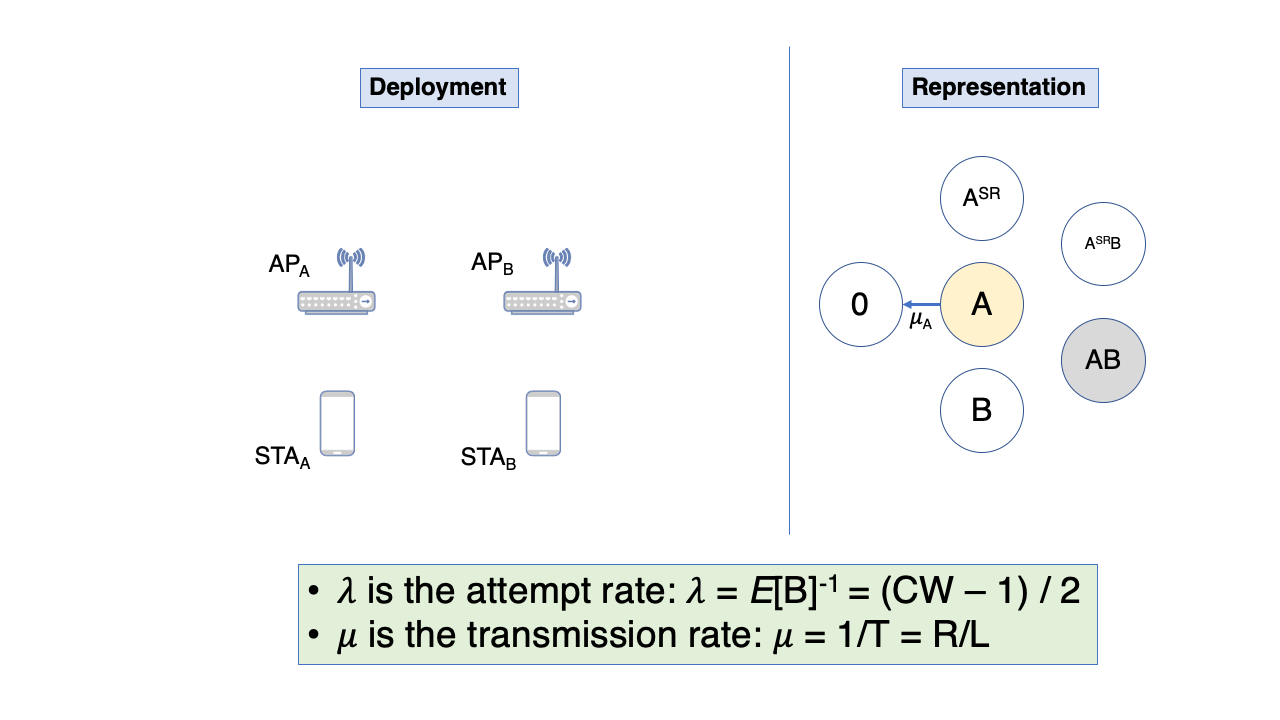
\includegraphics[width=\textwidth,height=\textheight,keepaspectratio]{img/anim4/frame-3}}
	\only<4>{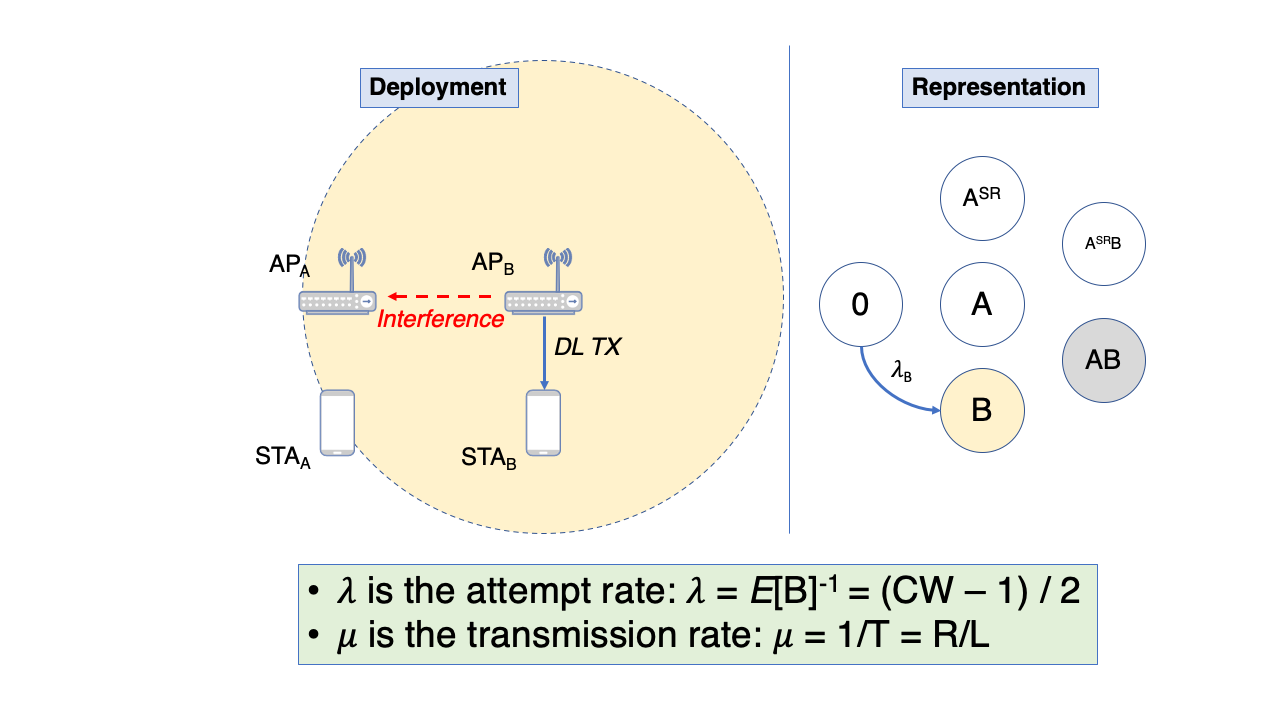
\includegraphics[width=\textwidth,height=\textheight,keepaspectratio]{img/anim4/frame-4}}
	\only<5>{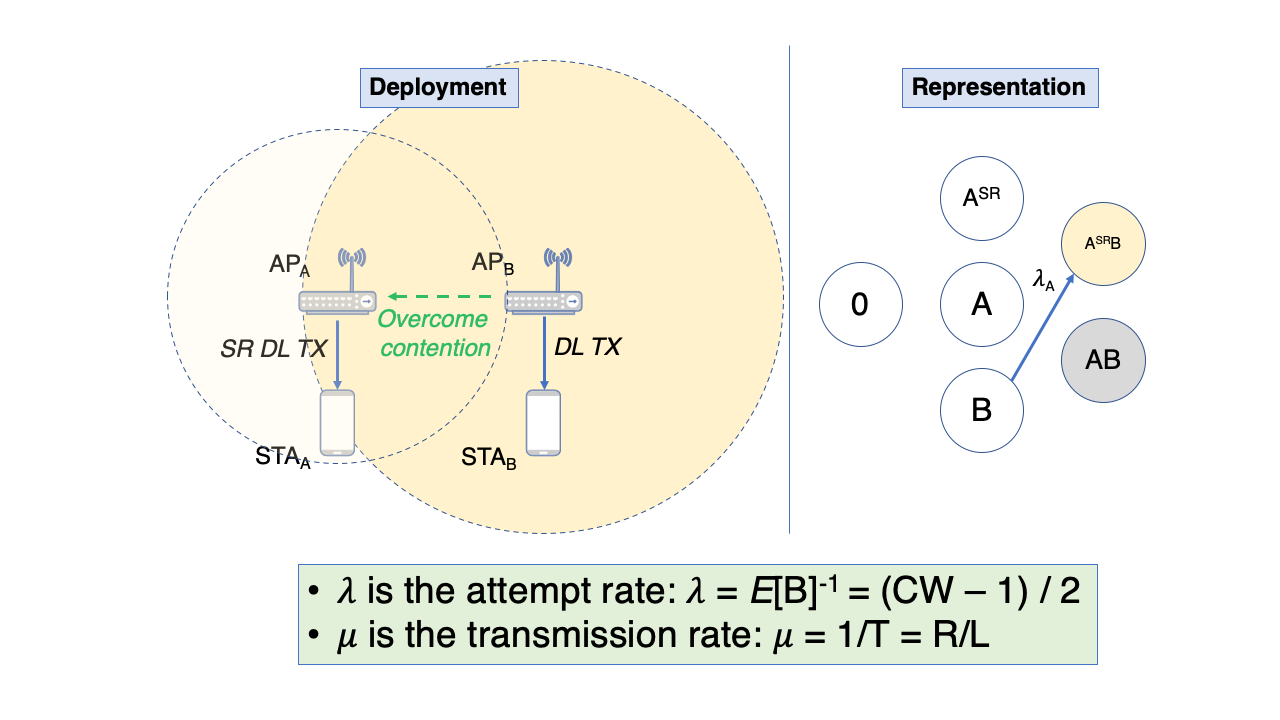
\includegraphics[width=\textwidth,height=\textheight,keepaspectratio]{img/anim4/frame-5}}
	\only<6>{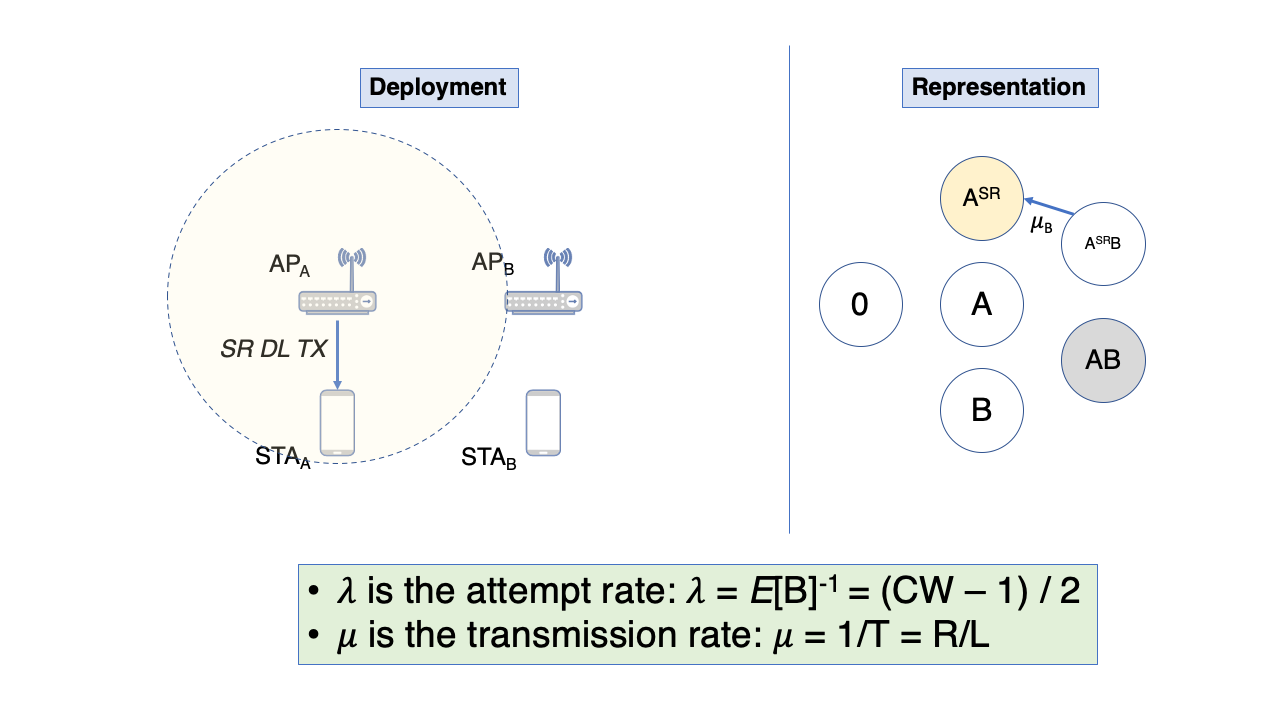
\includegraphics[width=\textwidth,height=\textheight,keepaspectratio]{img/anim4/frame-6}}
	\only<7>{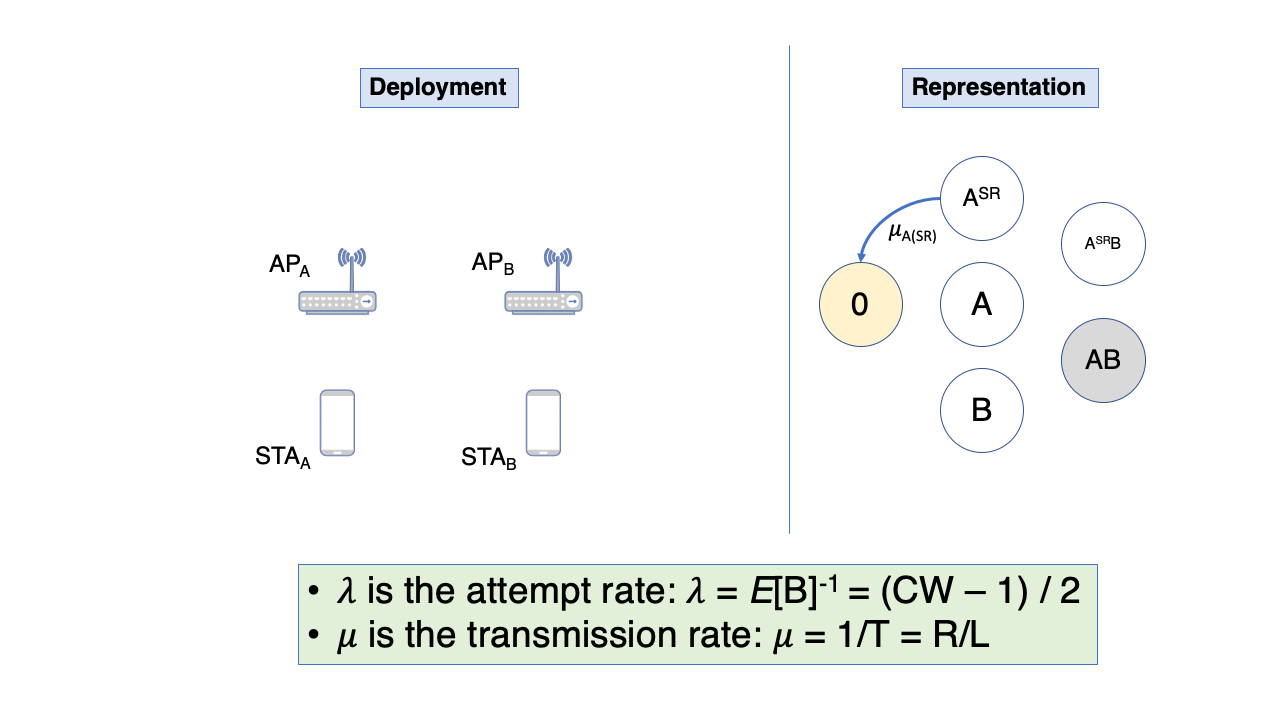
\includegraphics[width=\textwidth,height=\textheight,keepaspectratio]{img/anim4/frame-7}}
\end{figure}
\end{frame}

\begin{frame}{Characterization of intelligent IEEE 802.11 WLANs}
\pause
\begin{columns}
	\begin{column}{6cm}
		\begin{block}{The Komondor simulator}
			\begin{itemize}		
				\item IEEE 802.11ax-oriented discrete-event simulator\footnote{ns-3 11ax available since late 2019}
				\item Fast performance \& ML
				\item Joint contribution
			\end{itemize}
		\end{block}
	\end{column}
	\begin{column}{5.5cm}
		\begin{figure}
			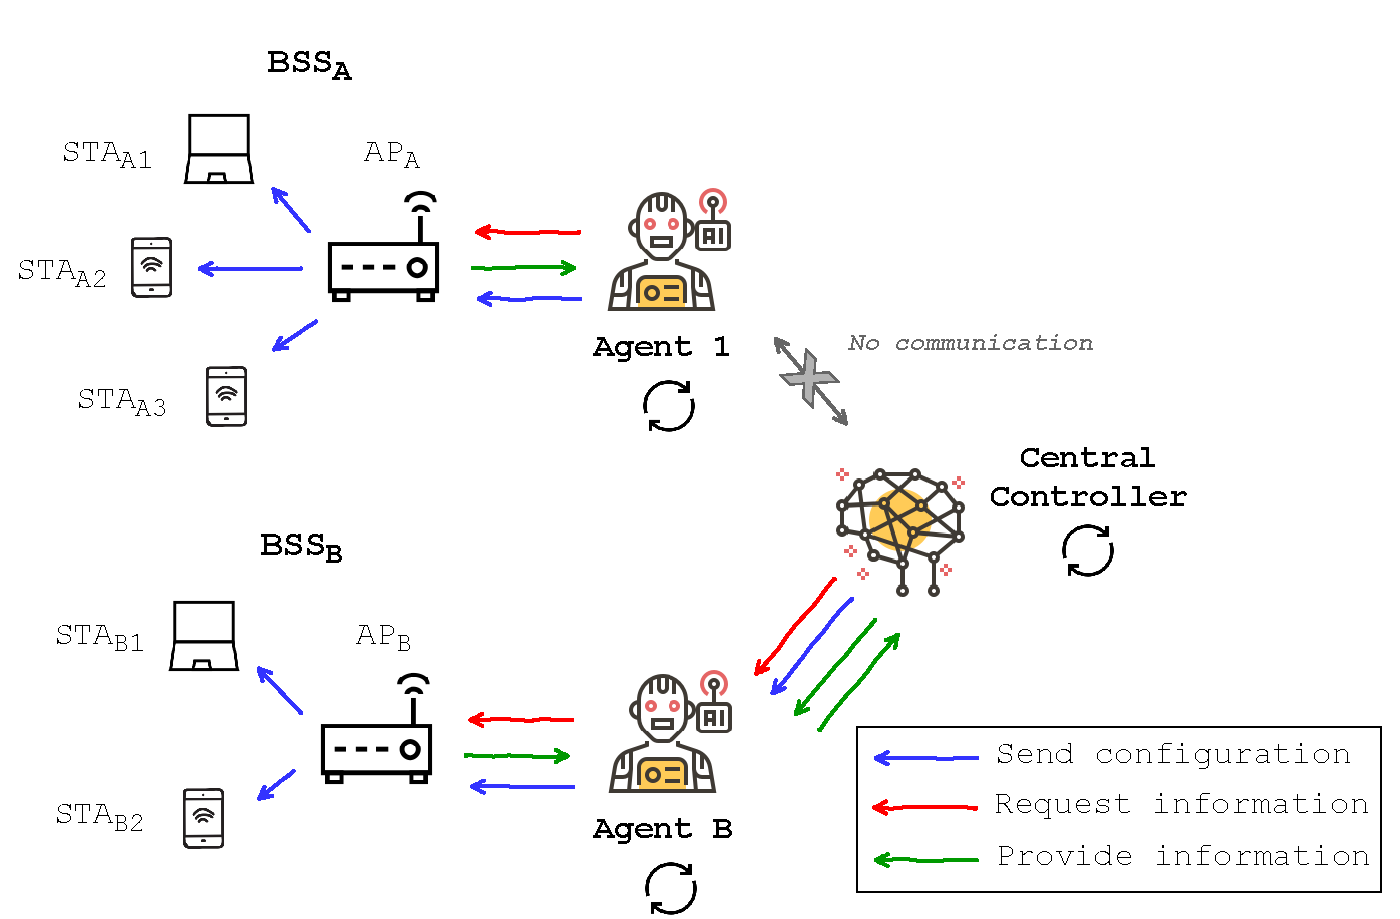
\includegraphics[width=\textwidth,height=\textheight,keepaspectratio]{img/overview_agents}
		\end{figure}
	\end{column}
\end{columns}
\begin{columns}
	\pause
	\begin{column}{6cm}
		\begin{alertblock}{Usage}
			\begin{itemize}
				\item Simulate OBSS/PD-based SR			
				\item Sequential learning
				\item Large-scale deployments
			\end{itemize}
		\end{alertblock}
	\end{column}
	\pause
	\vspace{-.5cm} 
	\begin{column}{5.5cm}
		\begin{center}
			\begin{minipage}{5cm}
				\begin{exampleblock}{}
					\centering
					Komondor is an open-source project: \url{https://github.com/wn-upf/Komondor}
				\end{exampleblock}
			\end{minipage}
		\end{center}
	\end{column}
\end{columns}
\end{frame}

%%%%%%%%%%%%%%
%%% Results
%%%%%%%%%%%%%%
\section[Findings]{Main Findings}

\subsection{}
\begin{frame}{Non-intrusive behavior of OBSS/PD-based SR}
\begin{center}
	\begin{minipage}{11cm}
		\begin{block}{}
			\centering
			 \textbf{Finding \#1:} SR is a fair mechanism that allows increasing the number of simultaneous transmissions in dense OBSSs, thus enhancing the throughput in high-interference scenarios
		\end{block}
	\end{minipage}
\end{center}
\vspace{-0.5cm}
\begin{columns}
	\pause
	\begin{column}{6.5cm}
		\begin{figure}
			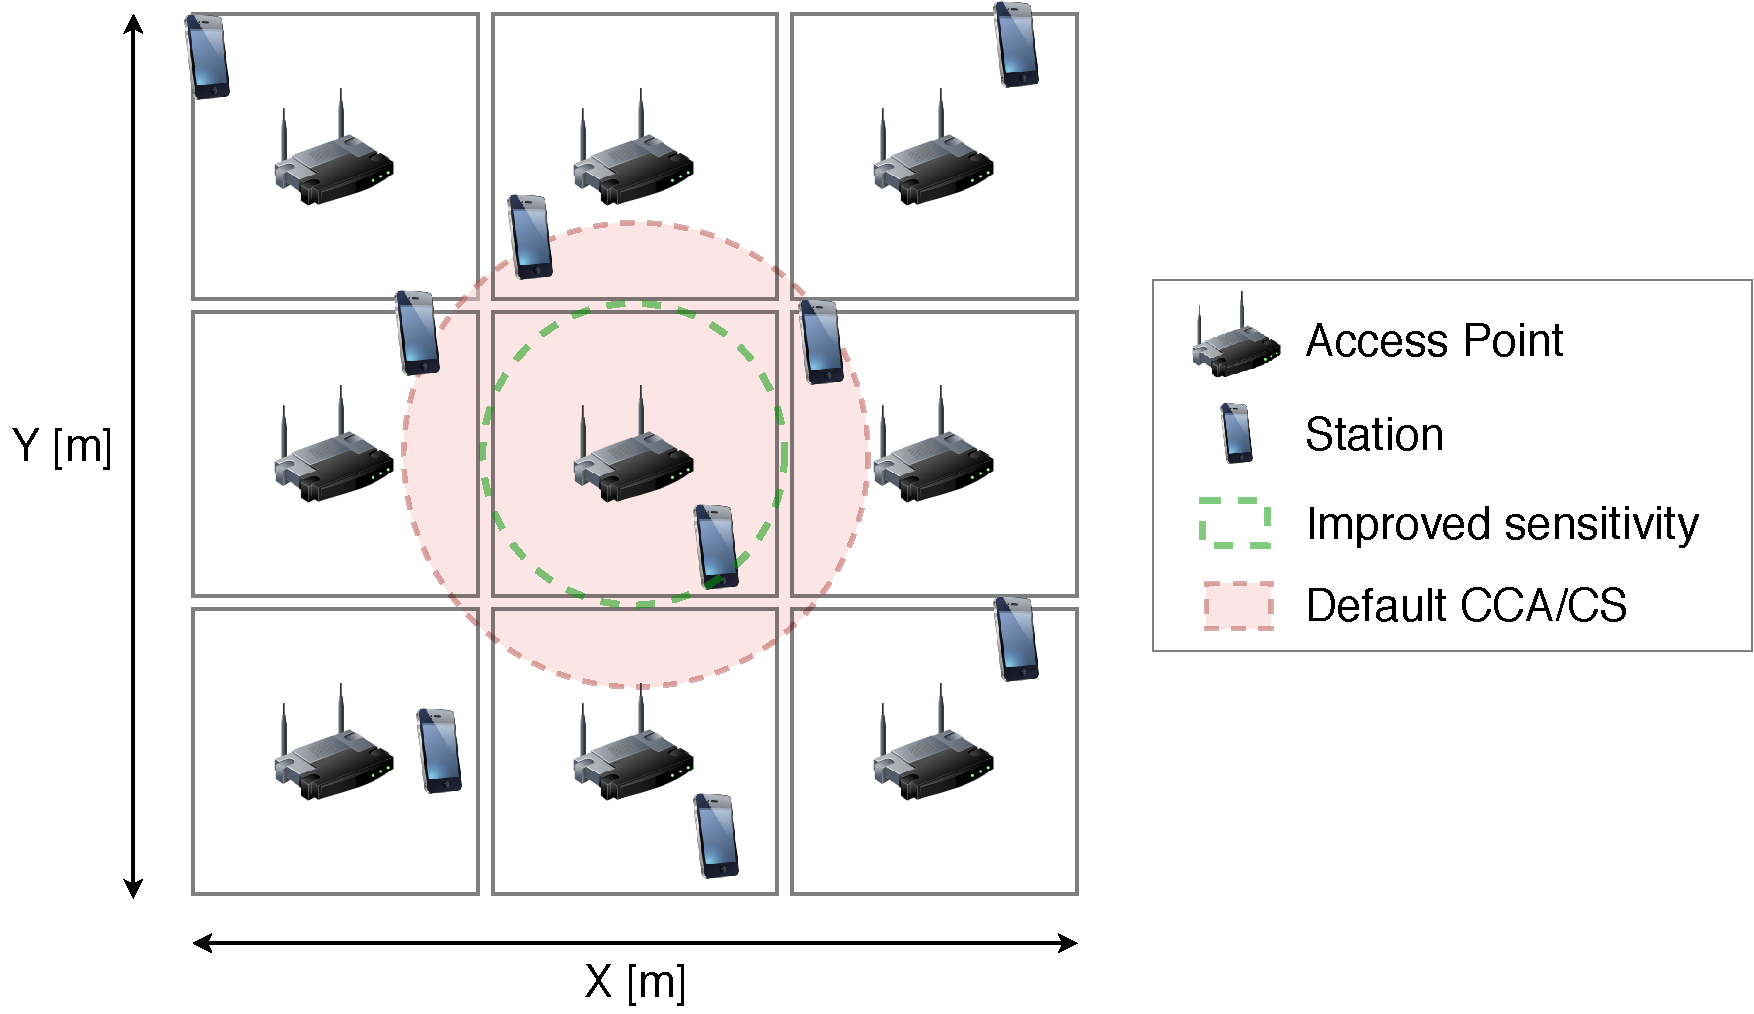
\includegraphics[width=.7\textwidth,height=\textheight,keepaspectratio]{img/random_scenario}
		\end{figure}
	\vspace{-0.65cm}
	%\fbox{\parbox{\textwidth}{
	\begin{itemize}
		\scriptsize
		\item Residential/Enterprise random scenario
		\item Different node densities
		\item Focus on BSS$_A$
		\item Compare performance of BSS$_A$ and rest of the BSSs
	\end{itemize}%}}
	\end{column}
	\pause
	\begin{column}{5.5cm}
		\begin{figure}
			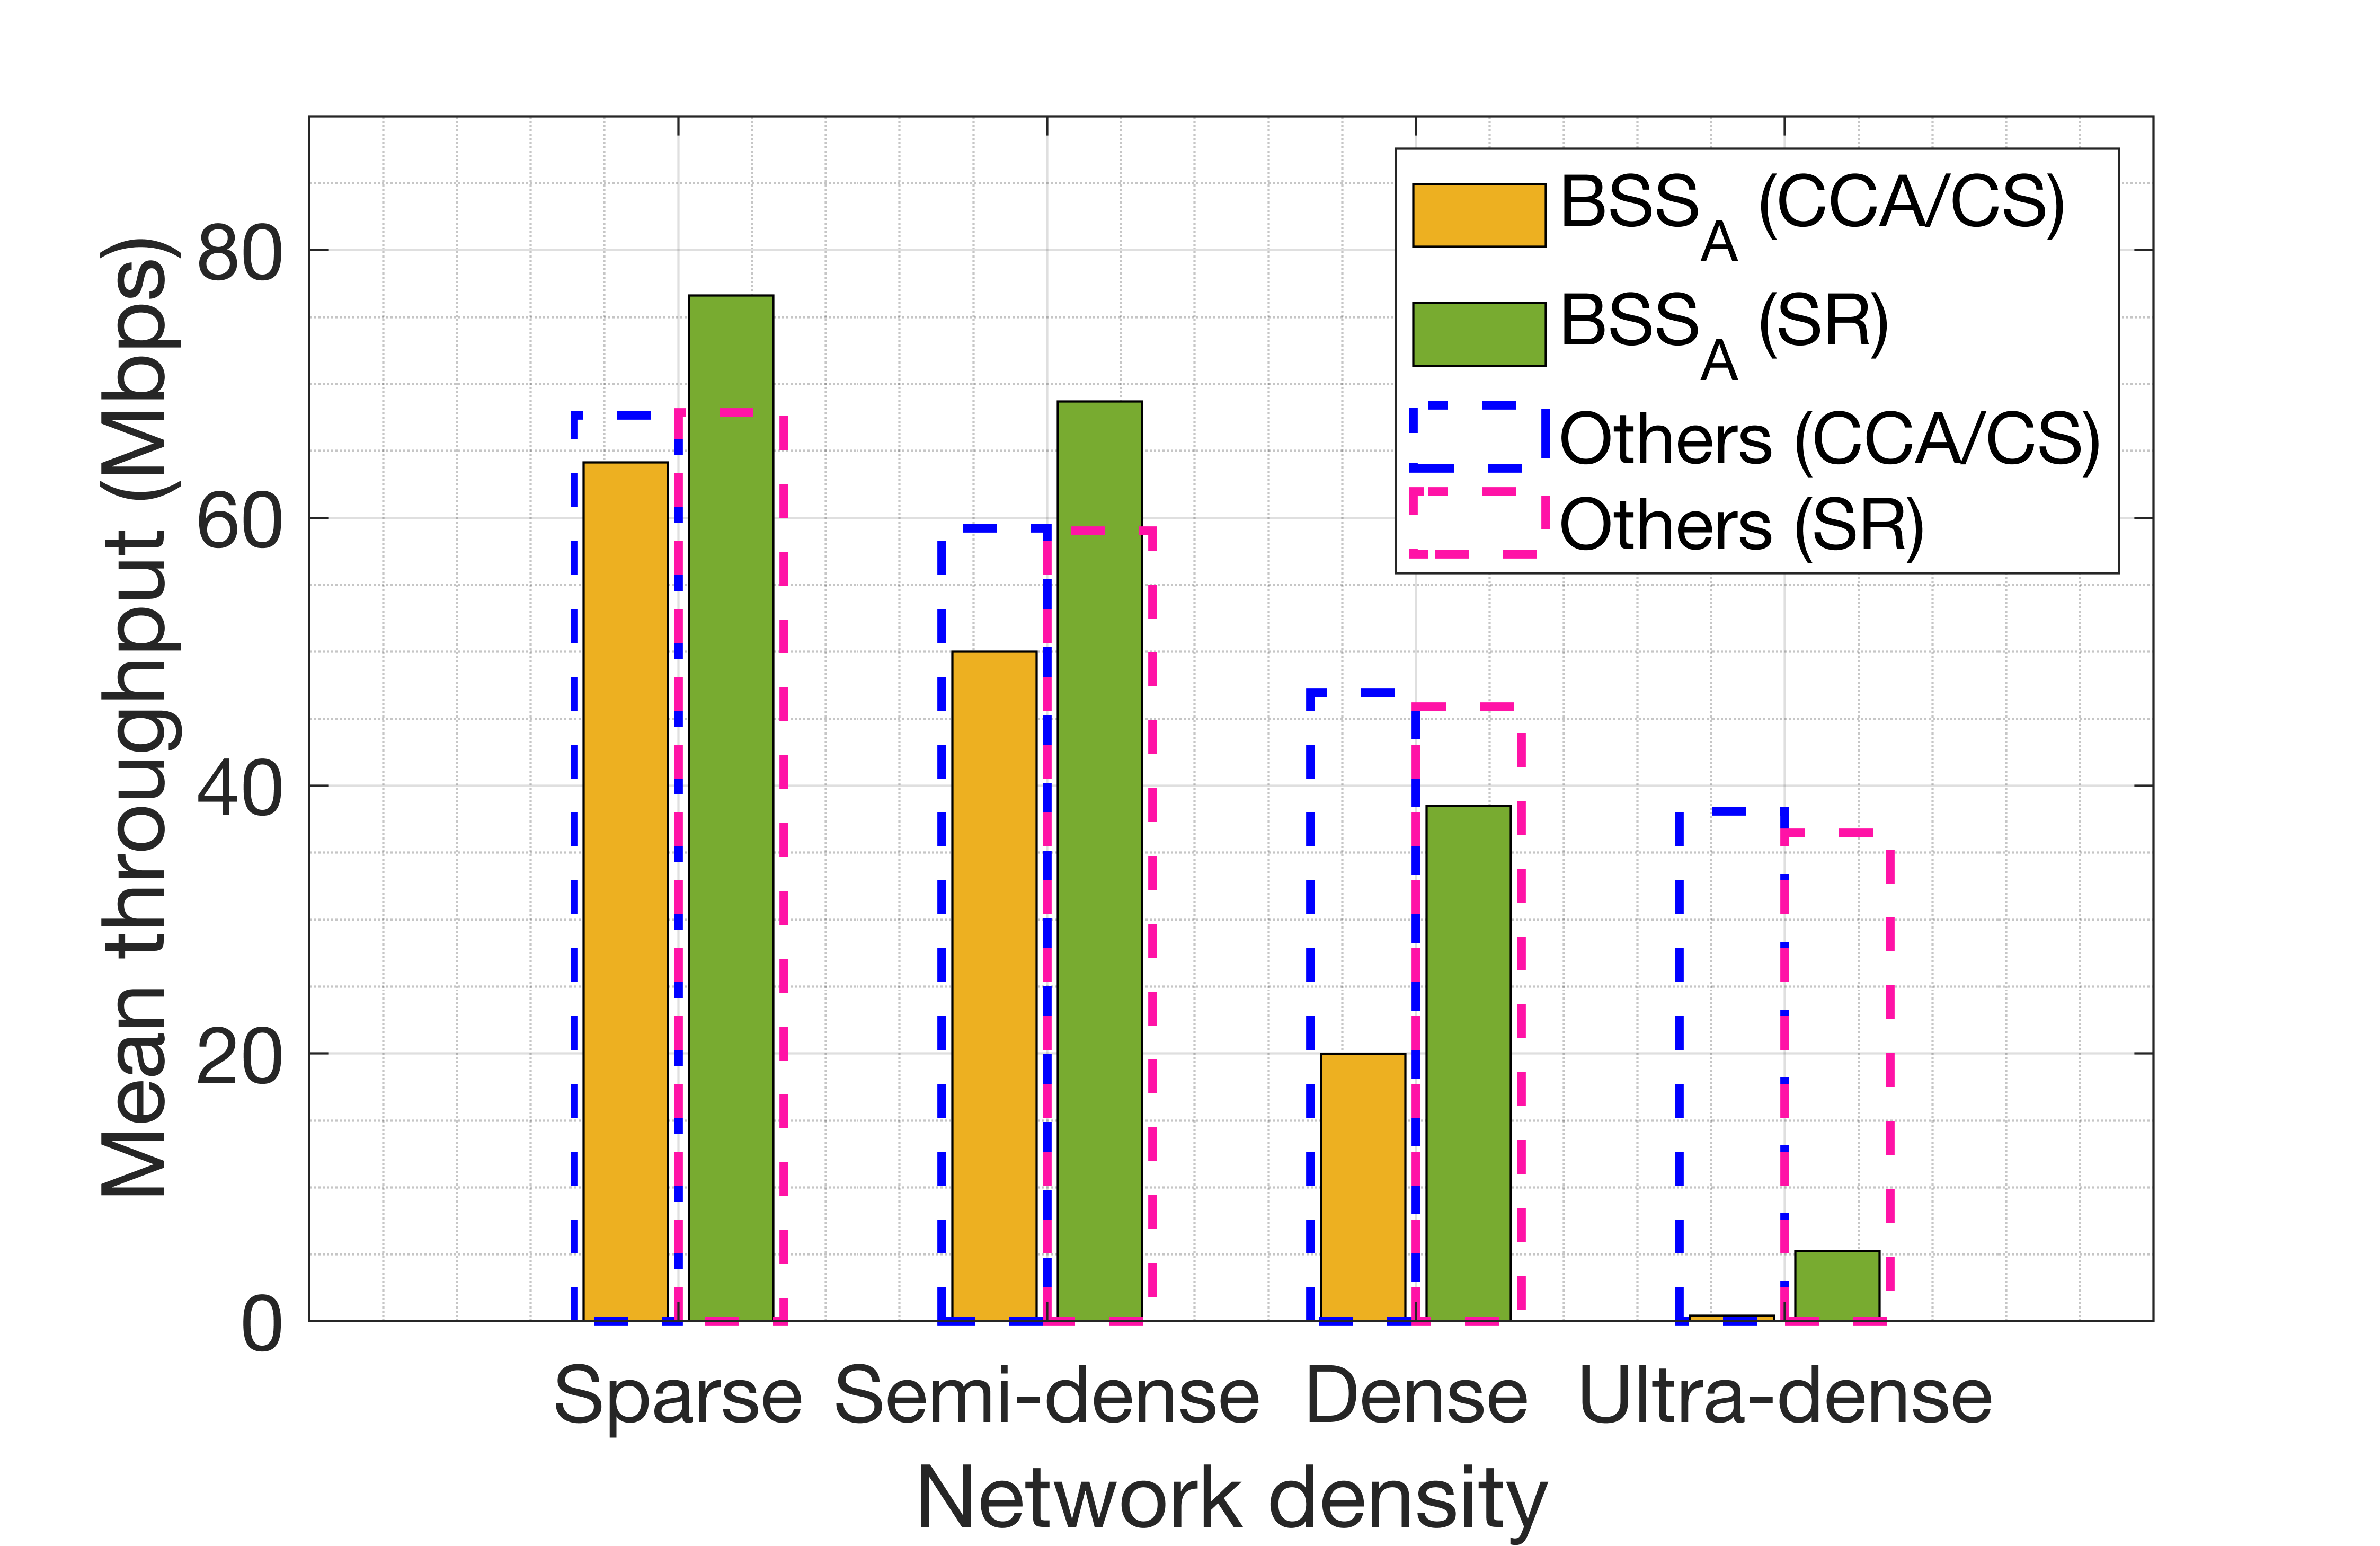
\includegraphics[width=1\textwidth,height=\textheight,keepaspectratio]{img/paper_1_throughput_per_density}	
		\end{figure}
	\end{column}
\end{columns}
\end{frame}

\subsection{}
\begin{frame}{Performance gains of OBSS/PD-based SR}

\begin{center}
	\begin{minipage}{10cm}
		\begin{block}{}
			\centering
			\textbf{Finding \#2:} SR allows to significantly improve the delay in dense deployments
		\end{block}
	\end{minipage}
\end{center}
\pause
\begin{columns}
	\begin{column}{4cm}
	%\fbox{\parbox{\textwidth}{
	\begin{itemize}
		\scriptsize
		\item Residential/Enterprise random scenario
		\item Variable density
		\item Variable traffic load
		\item Focus on BSS$_A$
		\item Focus on the delay
	\end{itemize}%}}
	\pause
	\end{column}
	\begin{column}{8.5cm}
		\begin{figure}
			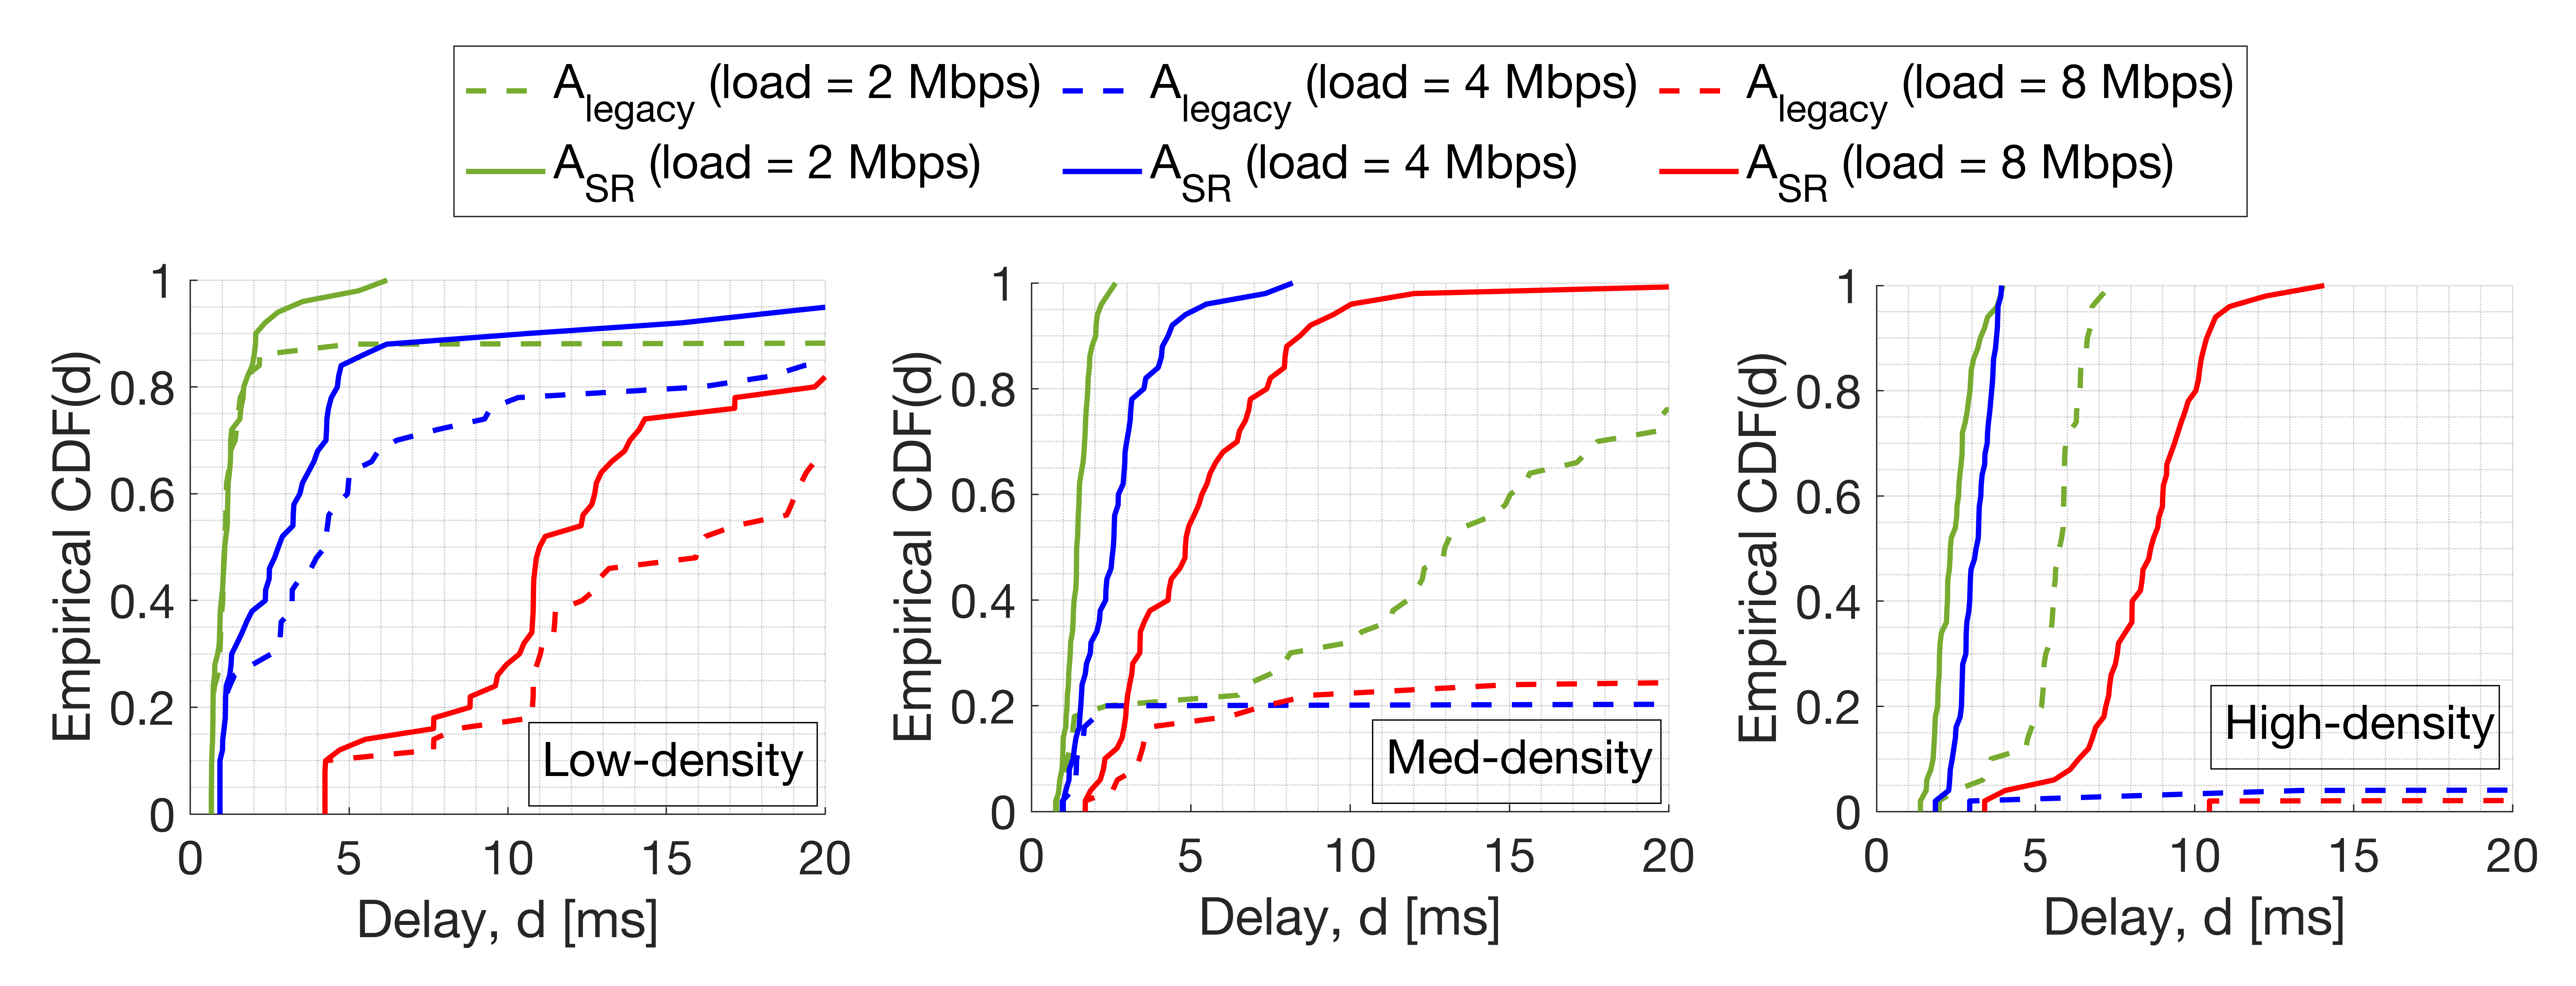
\includegraphics[width=1\textwidth,height=\textheight,keepaspectratio]{img/paper_2_delay}	
		\end{figure}
	\end{column}
\end{columns}

\end{frame}

%\begin{itemize}
%	\only<1>{\item \textbf{IEEE 802.11ax SR is kind with legacy devices
%	\item Increase the number of simultaneous tx in a dense OBSS}
%	\item \textcolor{gray}{Increase the number of simultaneous tx in a dense OBSS}
%	\item \textcolor{gray}{Throughput vs delay gains}
%	\item \textcolor{gray}{Performance gains are limited by lack of coordination}}
%	\only<2>{\item \textcolor{gray}{IEEE 802.11ax SR is kind with legacy devices}
%	\item \textcolor{gray}{Increase the number of simultaneous tx in a dense OBSS}
%	\item \textbf{Throughput vs delay gains}
%	\item \textcolor{gray}{Performance gains limited by lack of coordination}}
%	\only<3>{\item \textcolor{gray}{IEEE 802.11ax SR is kind with legacy devices}
%	\item \textcolor{gray}{Increase the number of simultaneous tx in a dense OBSS}
%	\item \textcolor{gray}{Throughput vs delay gains}
%	\item \textbf{Performance gains limited by lack of coordination}}
%\end{itemize}	
%
%\vspace{-.95cm}
%\only<1>{\begin{columns}
%	\begin{column}{5cm}
%		%\vspace{-.1cm}
%		\begin{figure}
%			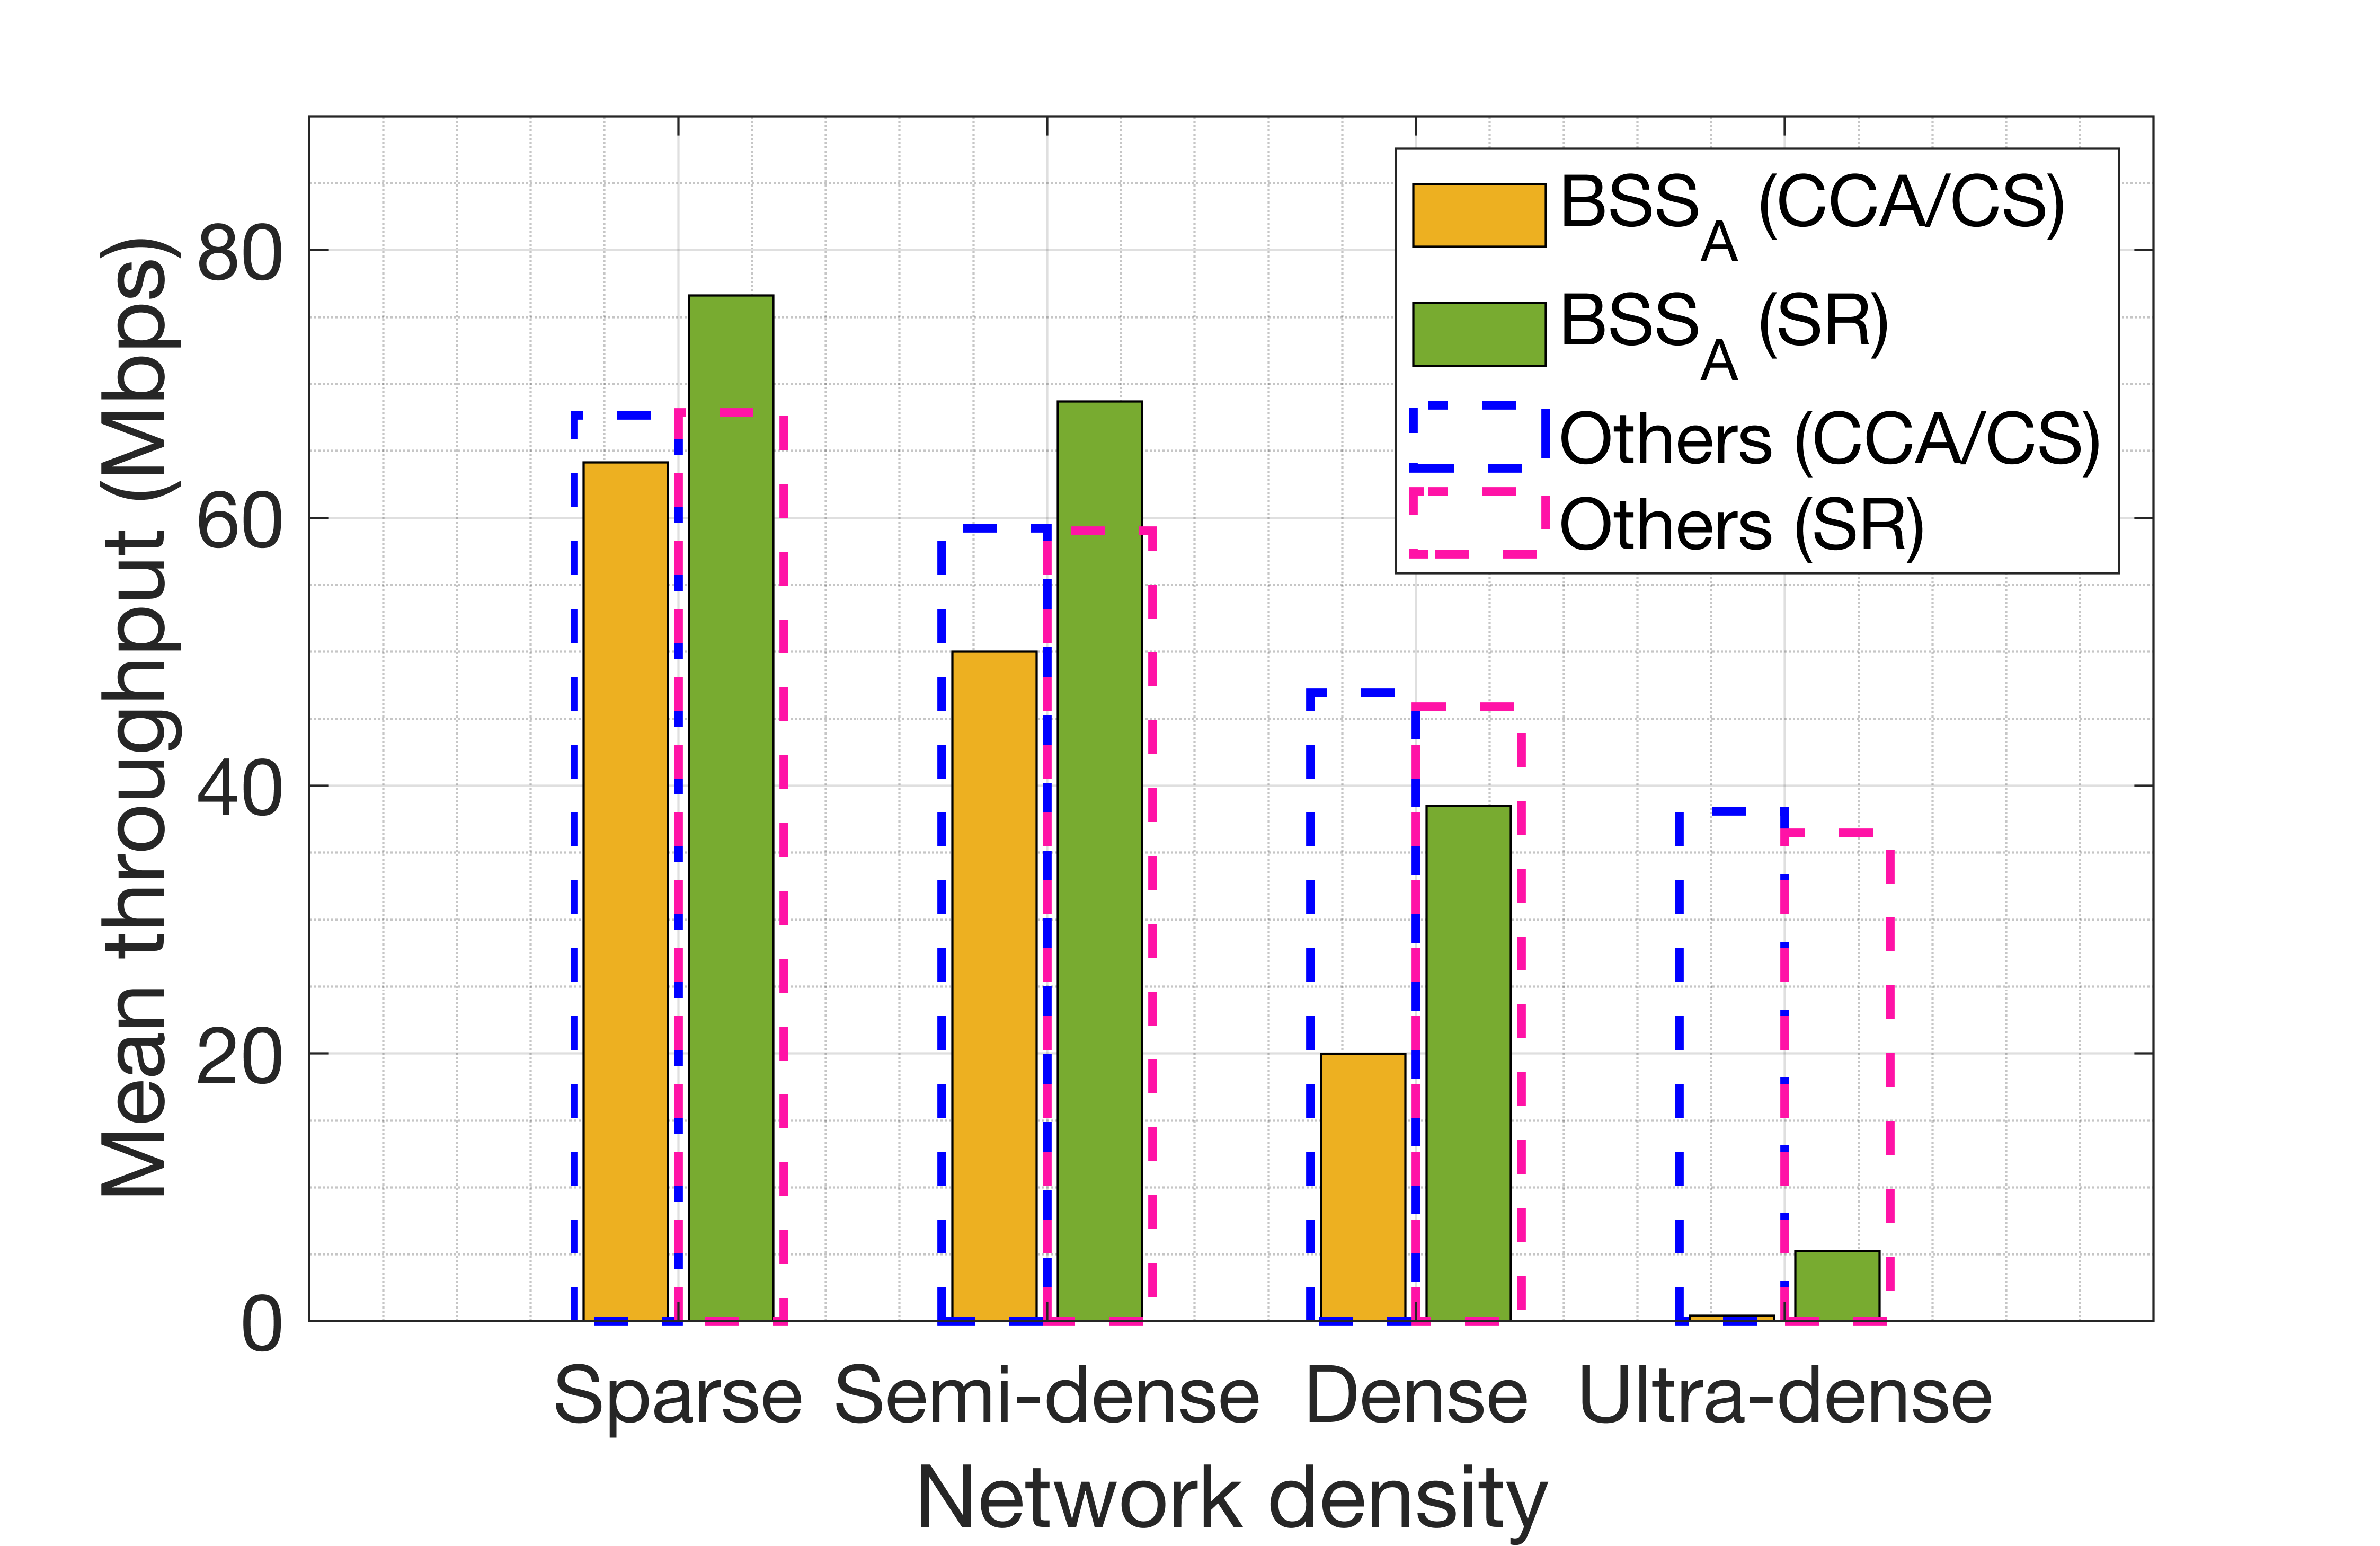
\includegraphics[width=1.3\textwidth,height=\textheight,keepaspectratio]{img/paper_1_throughput_per_density}	\end{figure}
%	\end{column}
%	\begin{column}{5cm}
%		\begin{figure}
%			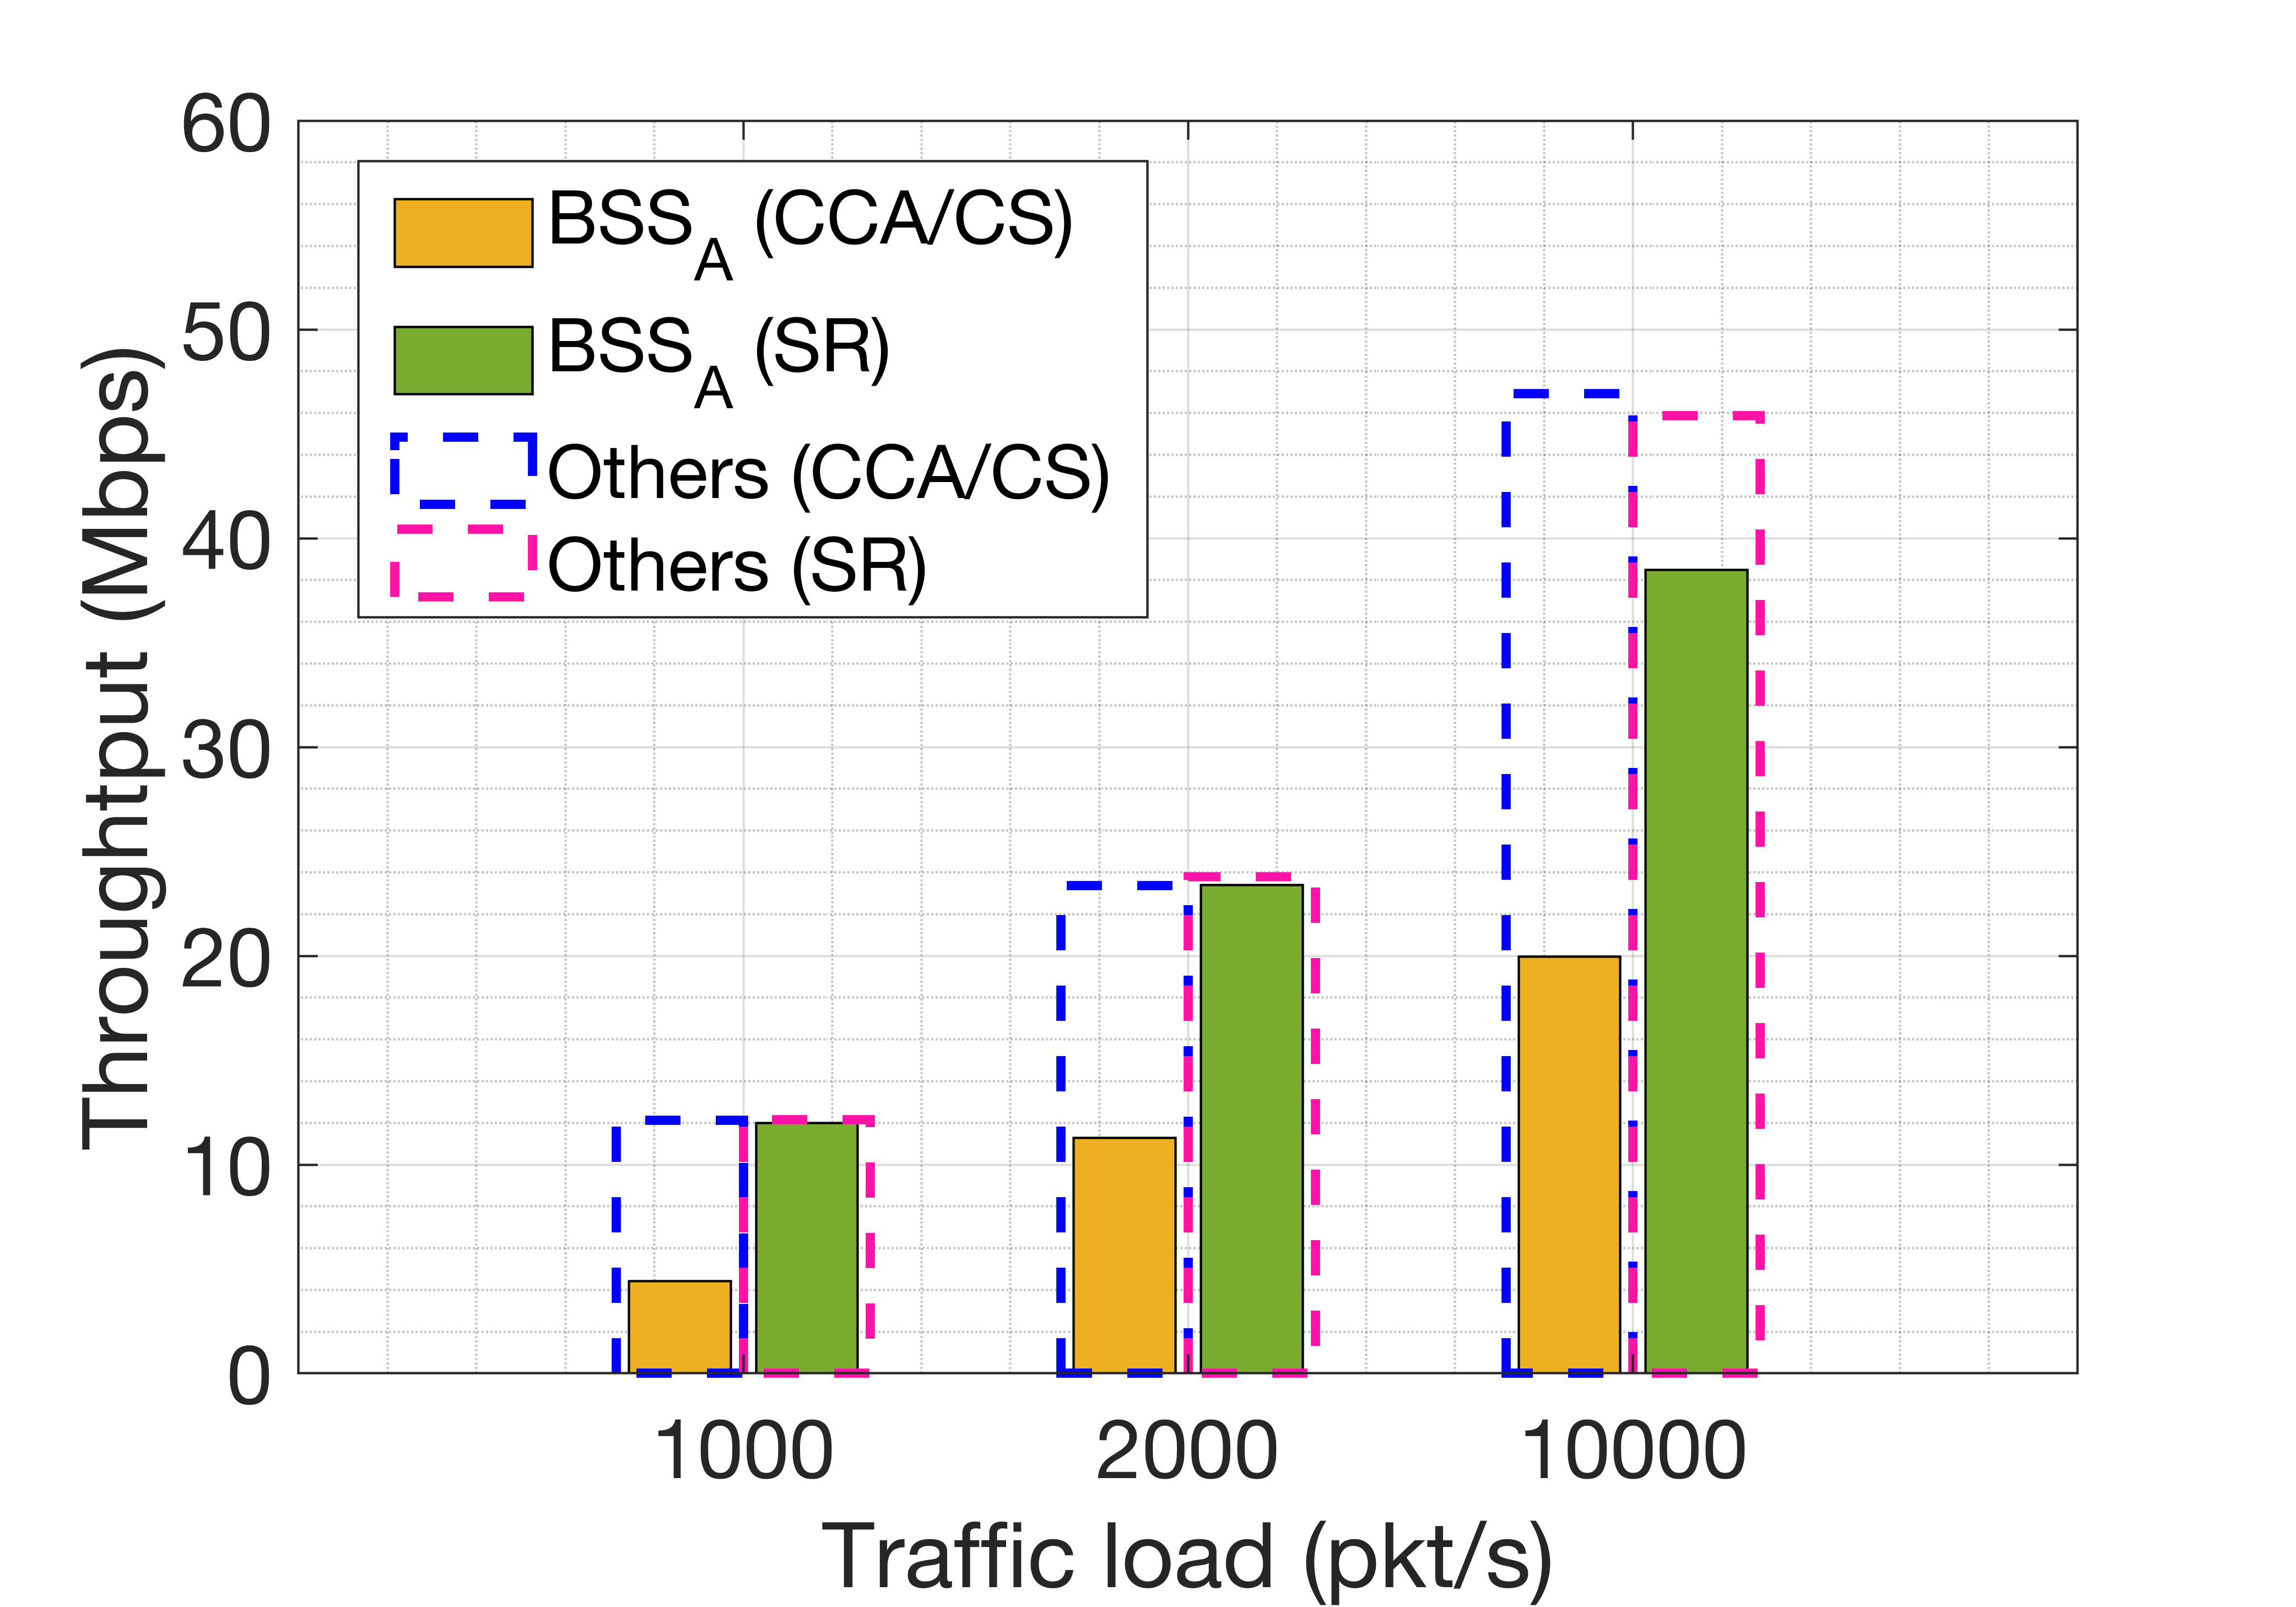
\includegraphics[width=1.2\textwidth,height=\textheight,keepaspectratio]{img/paper_1_throughput_per_load}
%		\end{figure}
%	\end{column}
%\end{columns}}
%
%\vspace{0.95cm}
%\only<2>{\begin{figure}
%	\includegraphics[width=.6\textwidth,height=\textheight,keepaspectratio]{img/paper_1_all}
%\end{figure}}
%
%\only<3>{\begin{columns}\begin{column}{6cm}
%		\vspace{-.55cm}
%		\begin{figure}
%			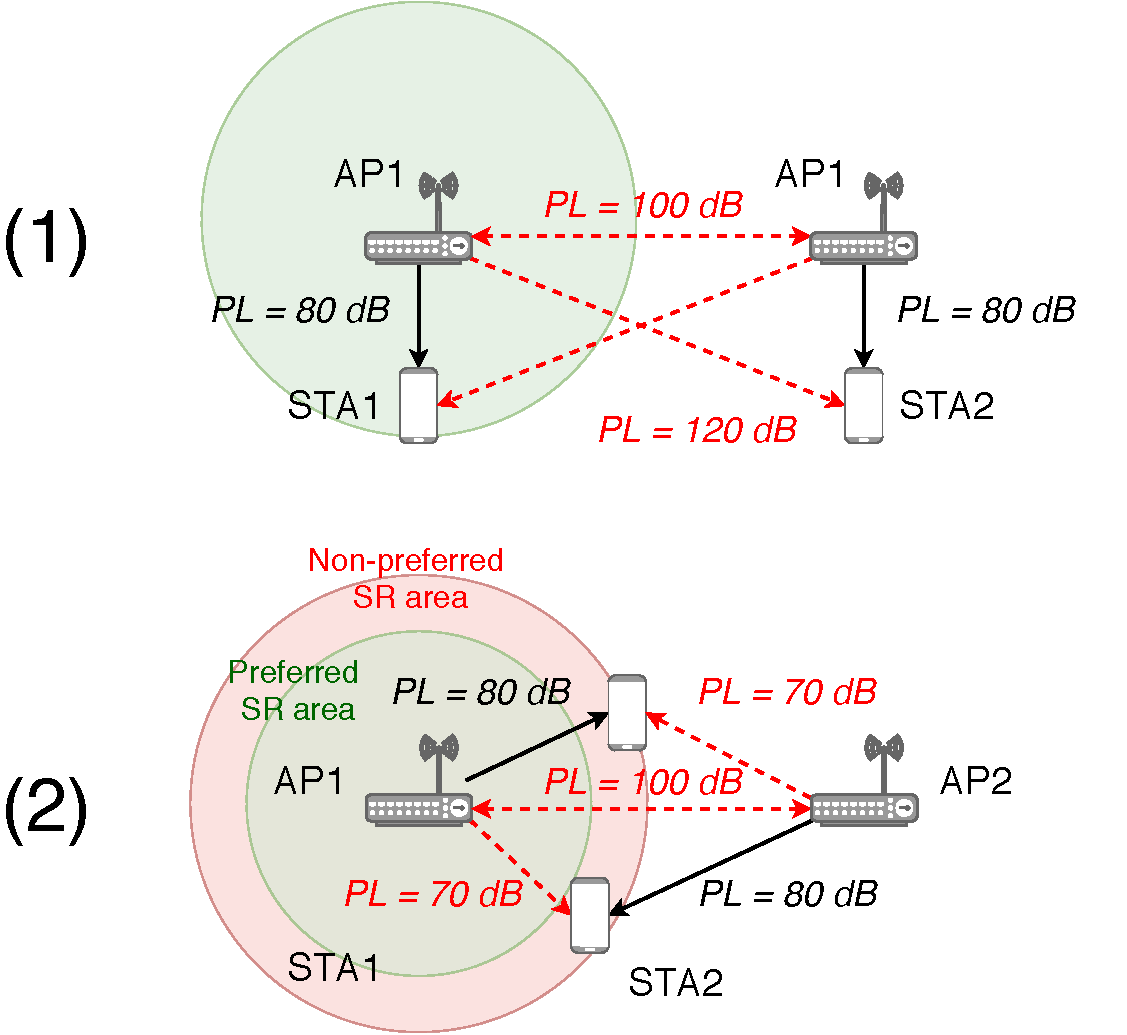
\includegraphics[width=.9\textwidth,height=\textheight,keepaspectratio]{img/paper_x_toy_deployments}
%		\end{figure}
%	\end{column}
%	\begin{column}{5cm}
%		\begin{figure}
%			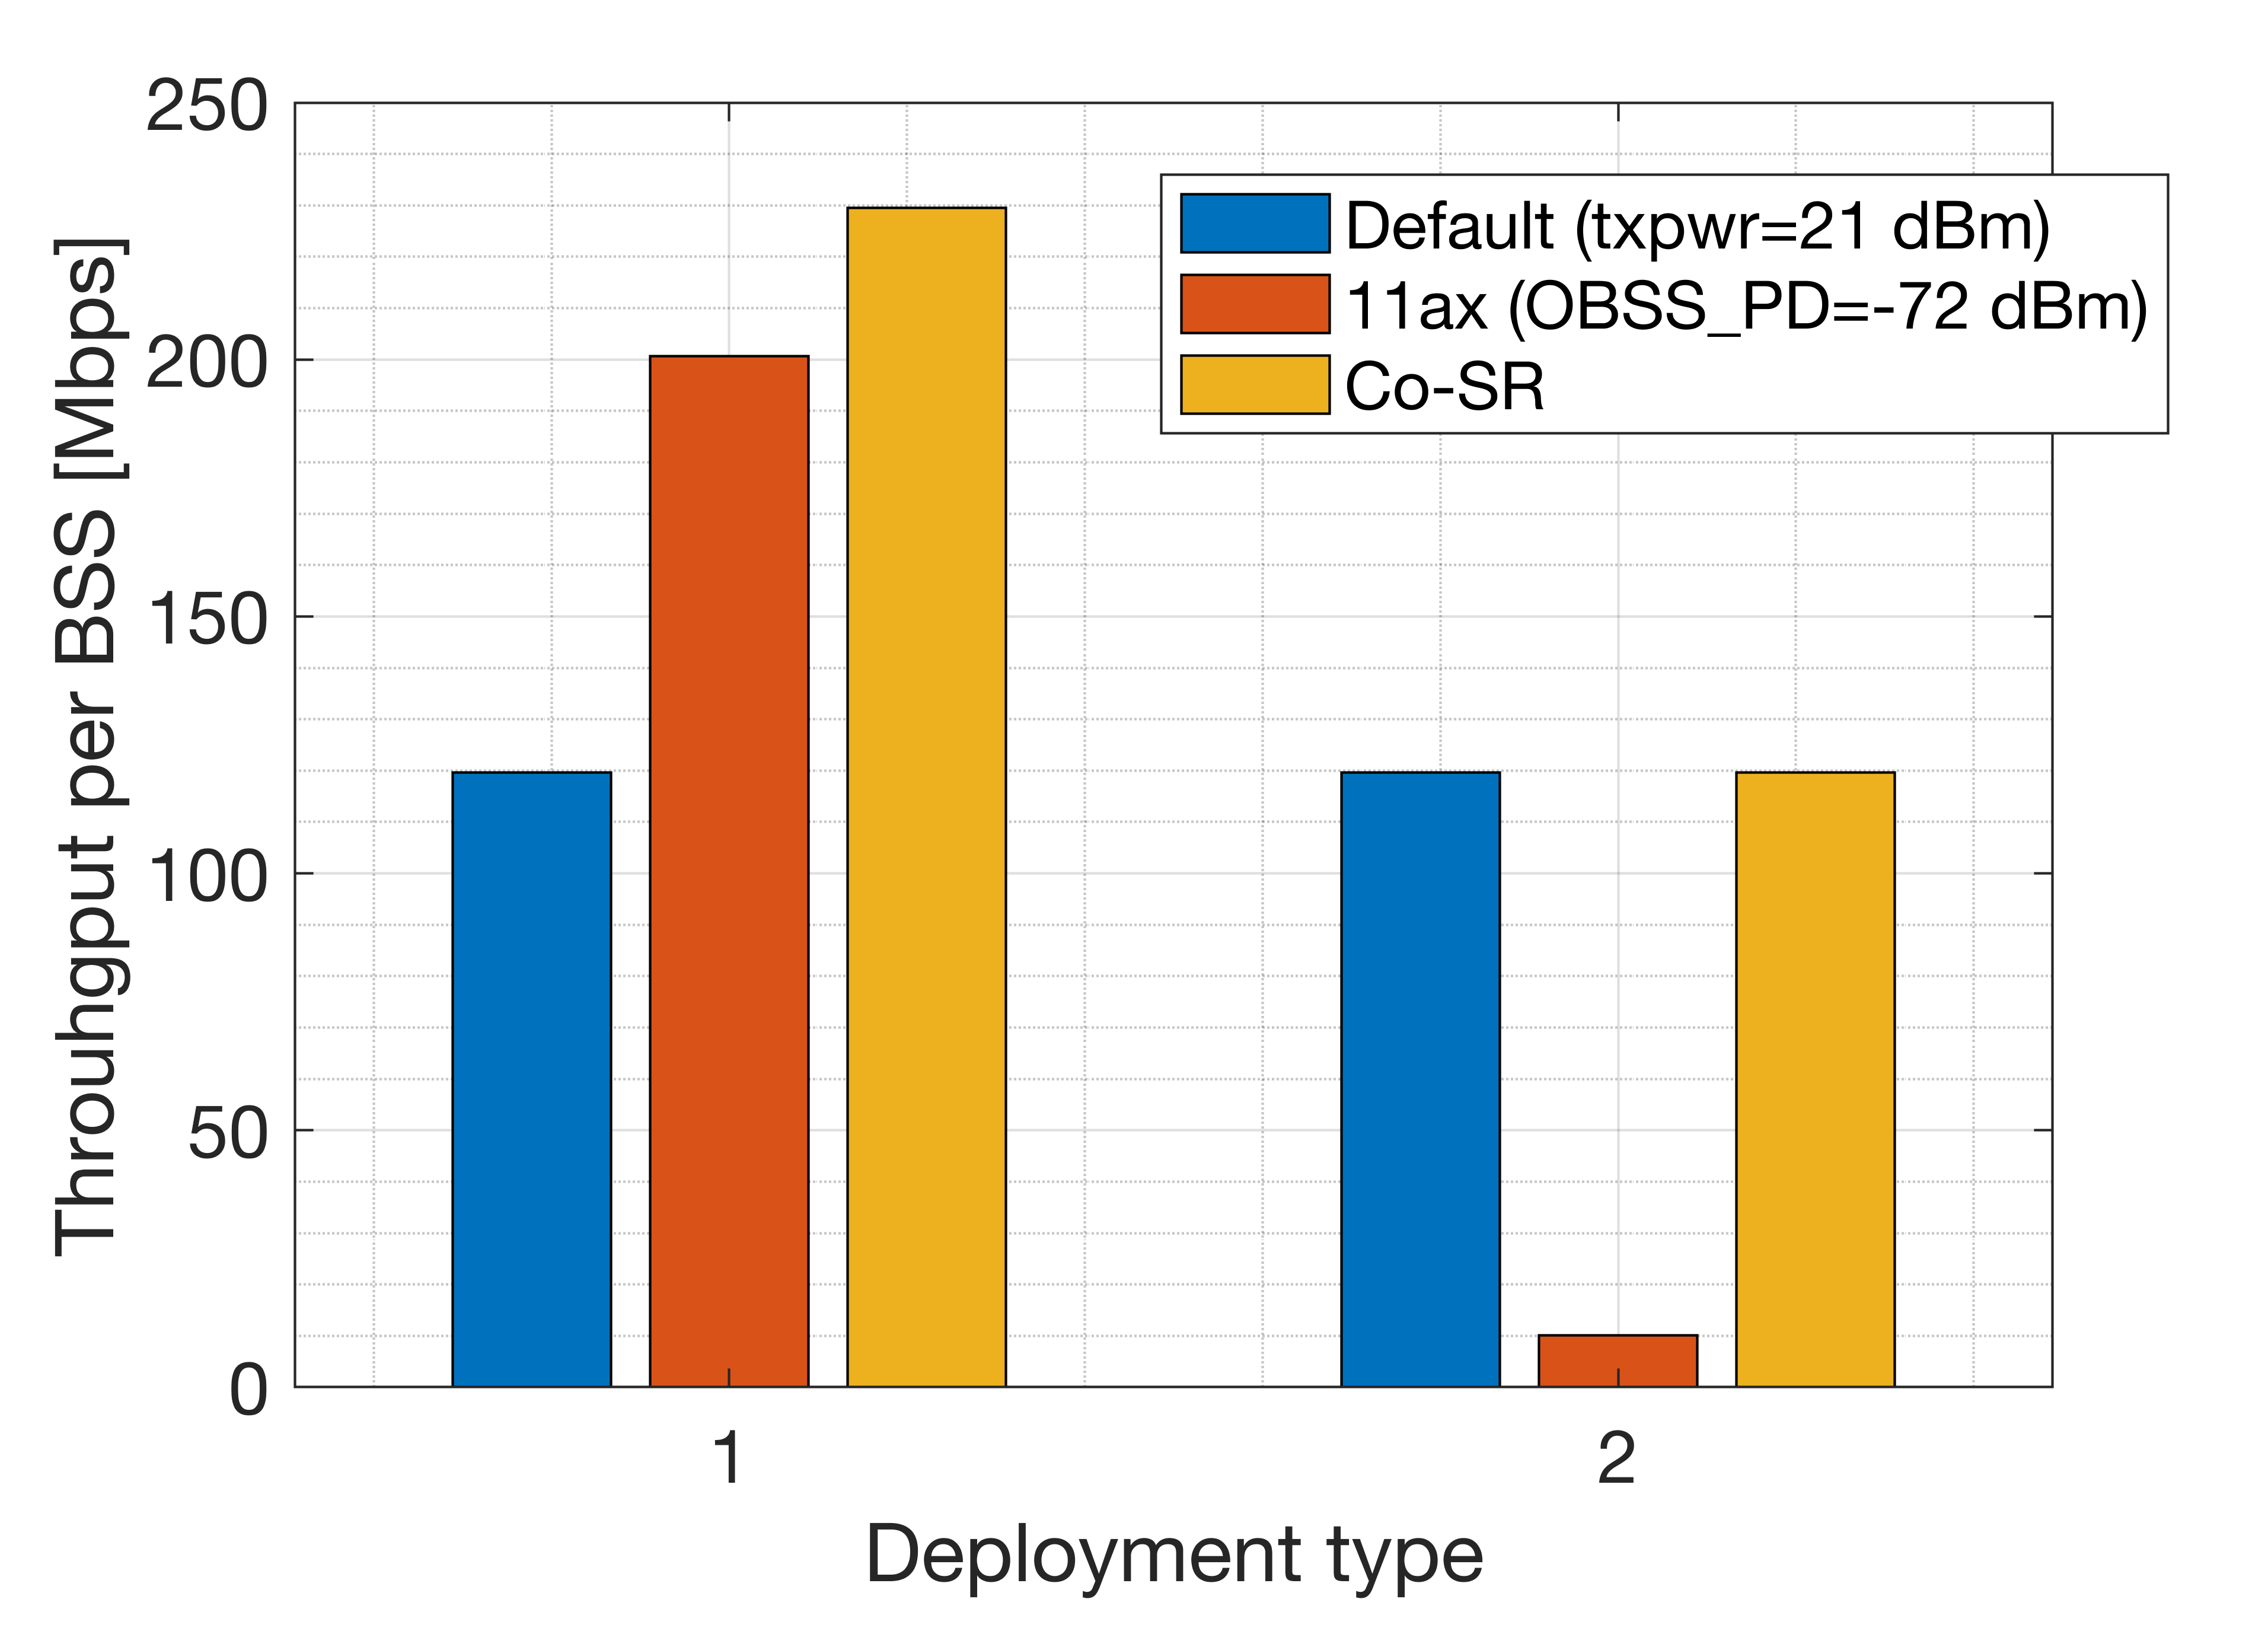
\includegraphics[width=1\textwidth,height=\textheight,keepaspectratio]{img/paper_x_results_toy_deployments}
%		\end{figure}
%	\end{column}
%\end{columns}}
%\end{frame}

\subsection{}
\begin{frame}{Considerations for adopting SL-based SR}

\begin{center}
	\begin{minipage}{11cm}
		\begin{block}{}
			\centering
			\textbf{Finding \#4:} Sequential learning mechanisms for multi-agent SR allow improving the performance of WLANs but may fail at finding a global optimum due to the competition among BSSs.
			%Sequential learning-based SR has limitations that stem from decentralization
		\end{block}
	\end{minipage}
\end{center}
\vspace{-.5cm}
\pause
\begin{columns}
	\begin{column}{6.5cm}
		\begin{figure}
			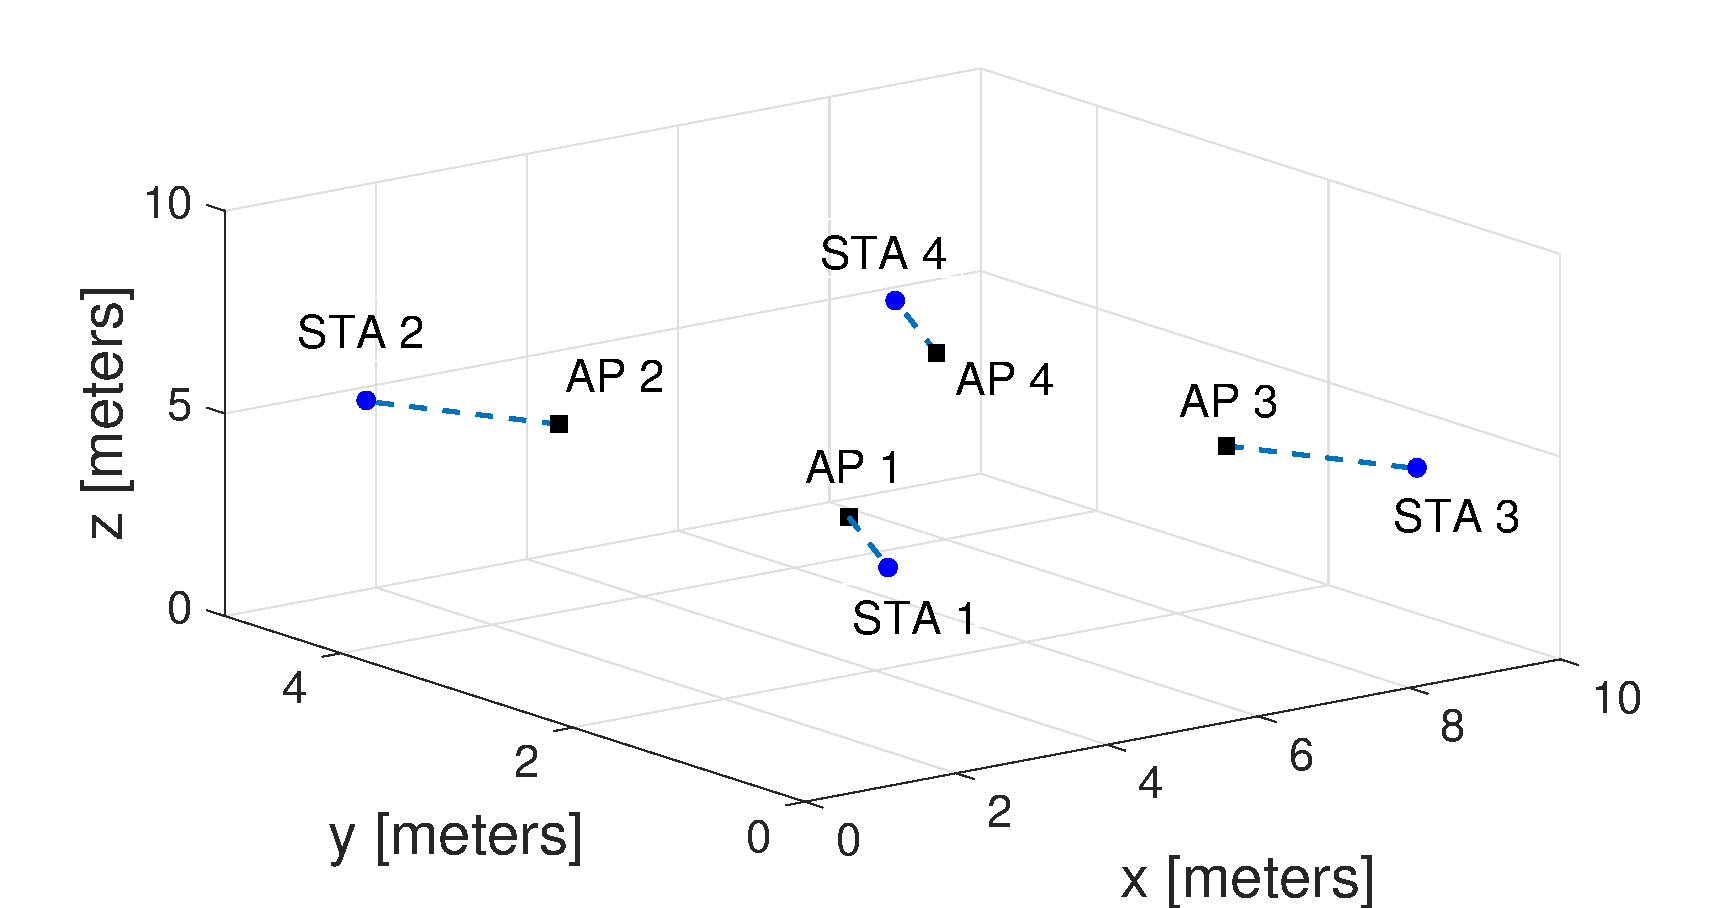
\includegraphics[width=.75\textwidth,height=\textheight,keepaspectratio]{img/4_WLANs_scenario-eps-converted-to}
		\end{figure}
	\vspace{-0.5cm}
	\begin{itemize}
		\scriptsize
		\item High interference regime
		\item Stateless Q-learning applied concurrently
		\item Local information only (selfish approach)
		\item Focus on competition
	\end{itemize}
\pause
	\end{column}
	\begin{column}{6.5cm}
		\begin{figure}
			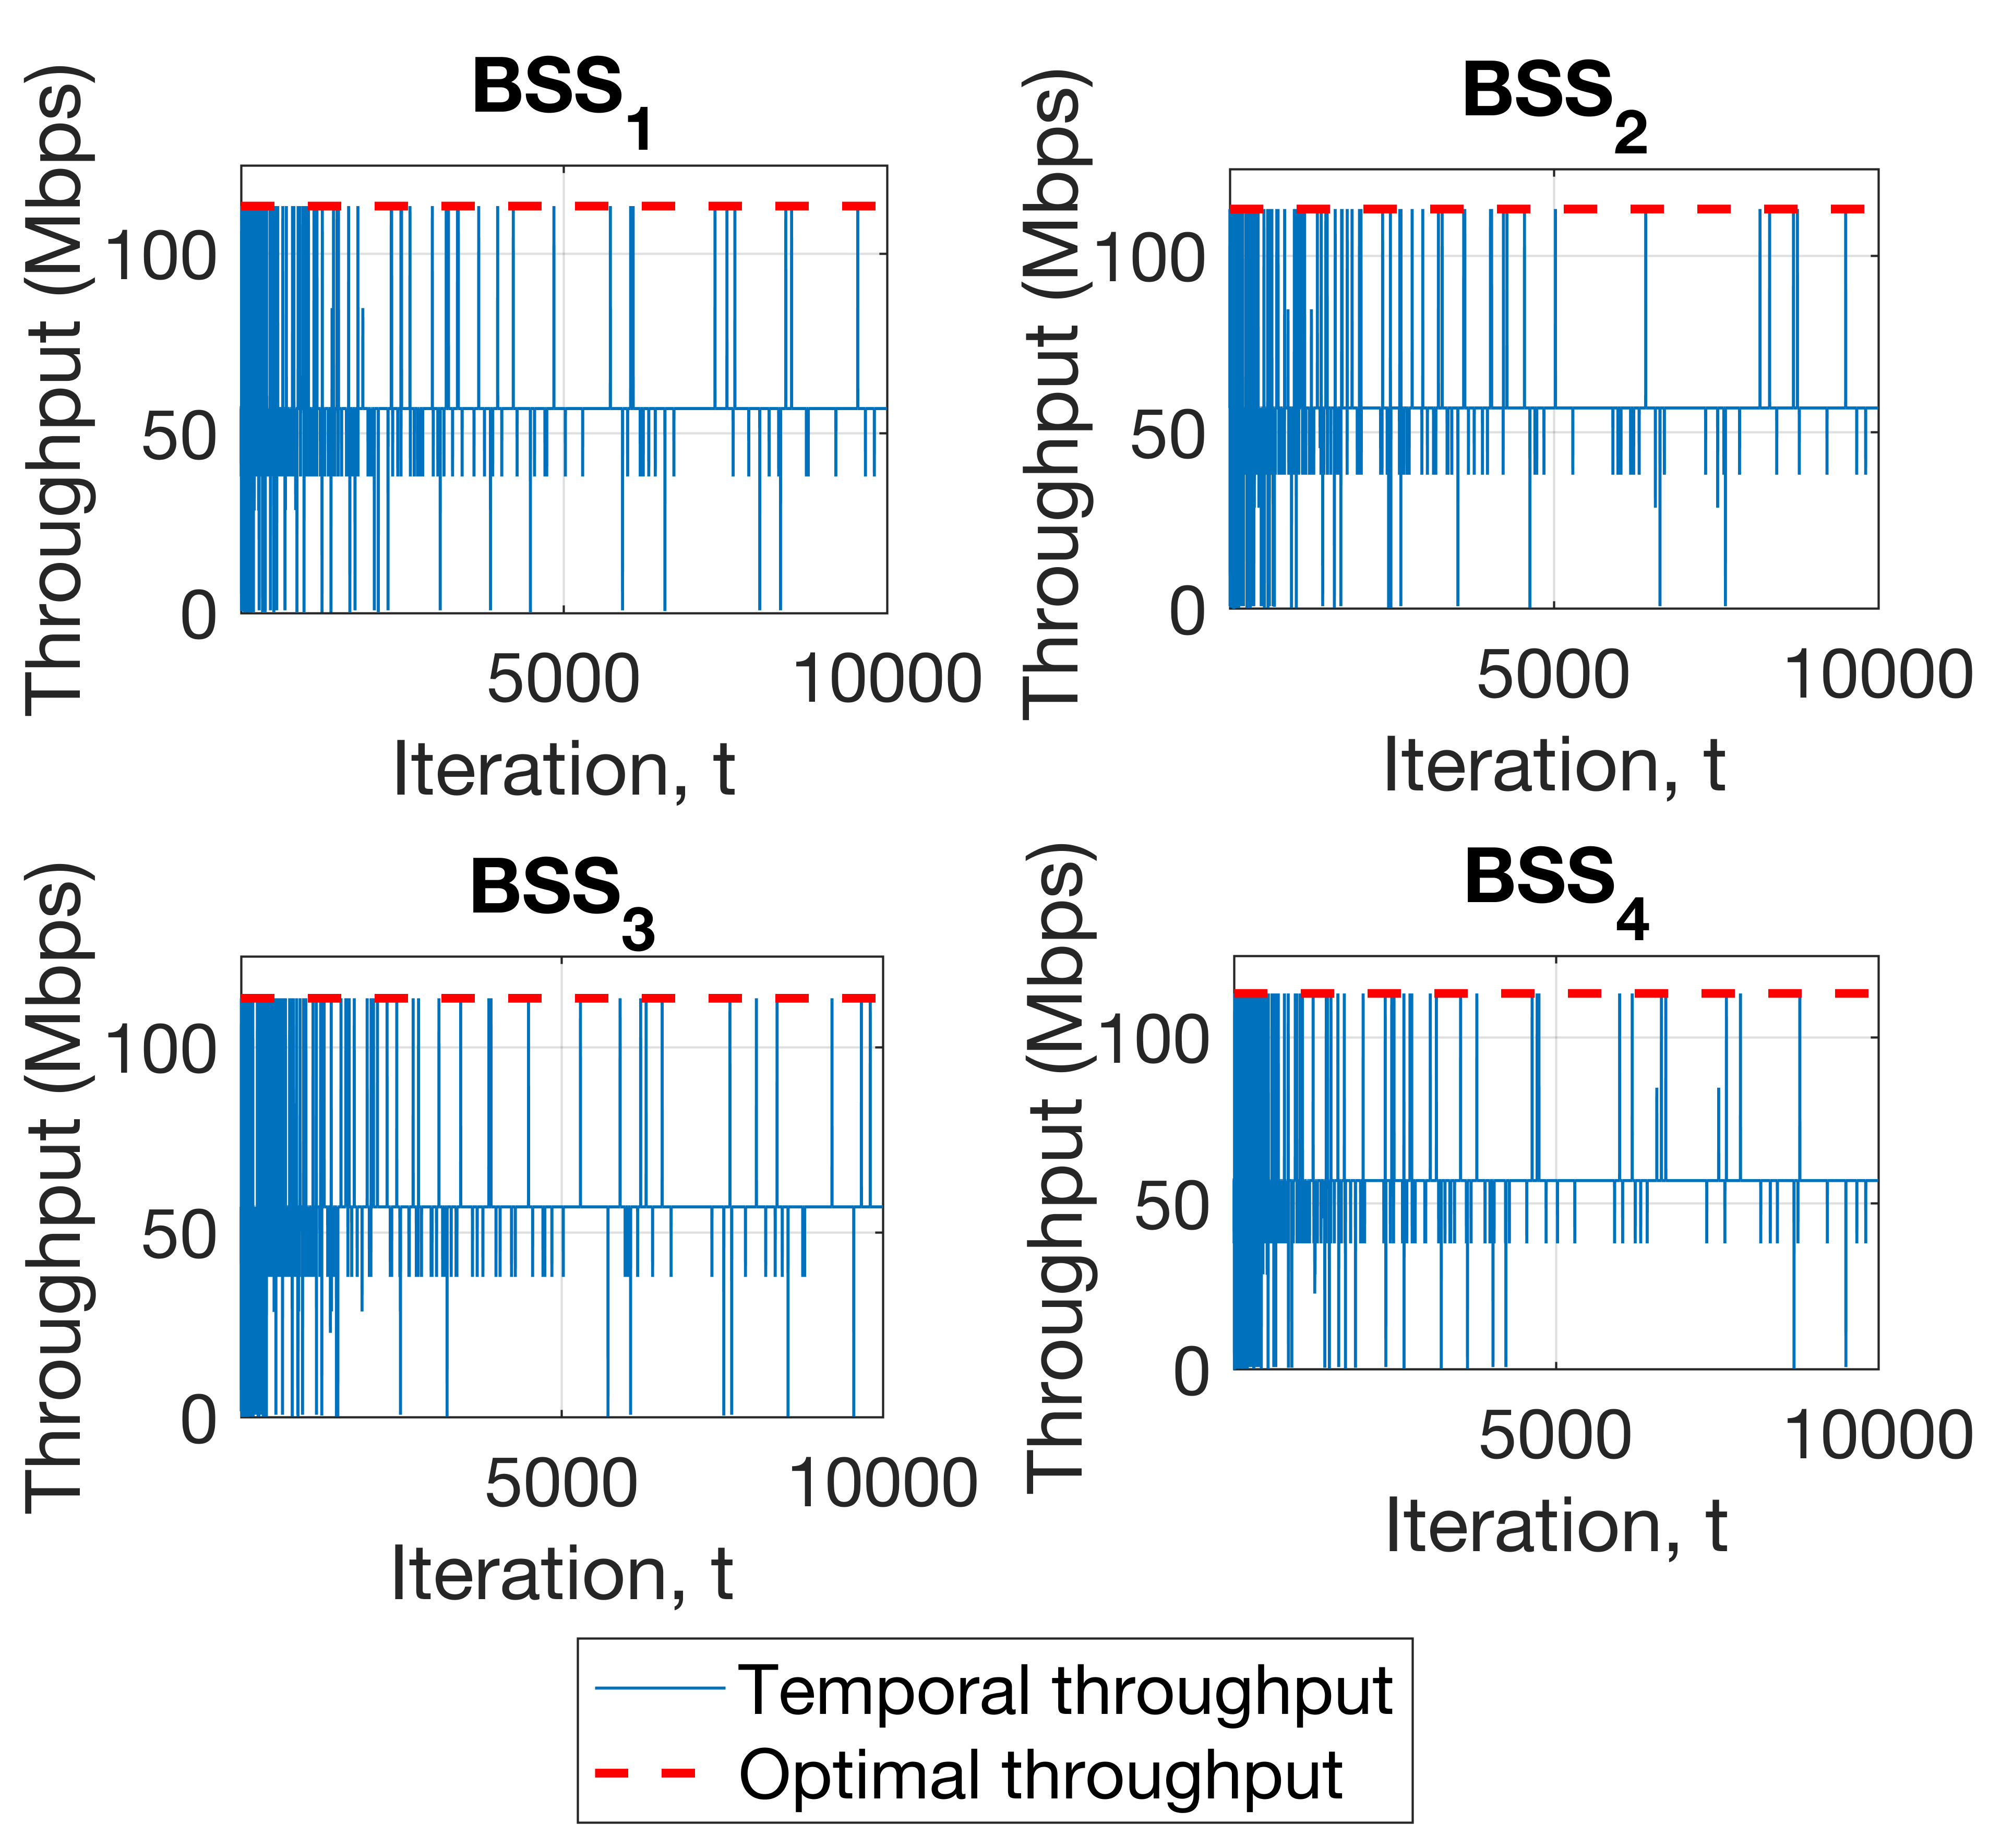
\includegraphics[width=.8\textwidth,height=\textheight,keepaspectratio]{img/temporal_individual_tpt_TS}	
		\end{figure}
	\end{column}
\end{columns}
\end{frame}

\subsection{}
\begin{frame}{Potential of sequential learning to address SR}
\vspace{-1cm}
\begin{center}
	\begin{minipage}{11cm}
		\begin{block}{}
			\centering
			\textbf{Finding \#5:} Collaborative rewards enhance fairness in decentralized settings, but neither ensure reaching an optimal global solution.			
			%Sequential learning-based SR is a robust method to improve the performance of  an OBSS
		\end{block}
	\end{minipage}
\end{center}
\pause
\begin{columns}
	\begin{column}{4.5cm}
		\begin{itemize}
			\scriptsize
			\item Random scenario
			\item Variable density
			\item MAB approach (Thompson sampling)
			\item Selfish vs Collaborative
			\item Short-term optimization (500 iterations)
			\item Focus on robustness
		\end{itemize}
	\end{column}
	\pause
	\hspace{0.25cm}			
	\begin{column}{8cm}
		\begin{columns}
			\begin{column}{4cm}
				\begin{figure}
					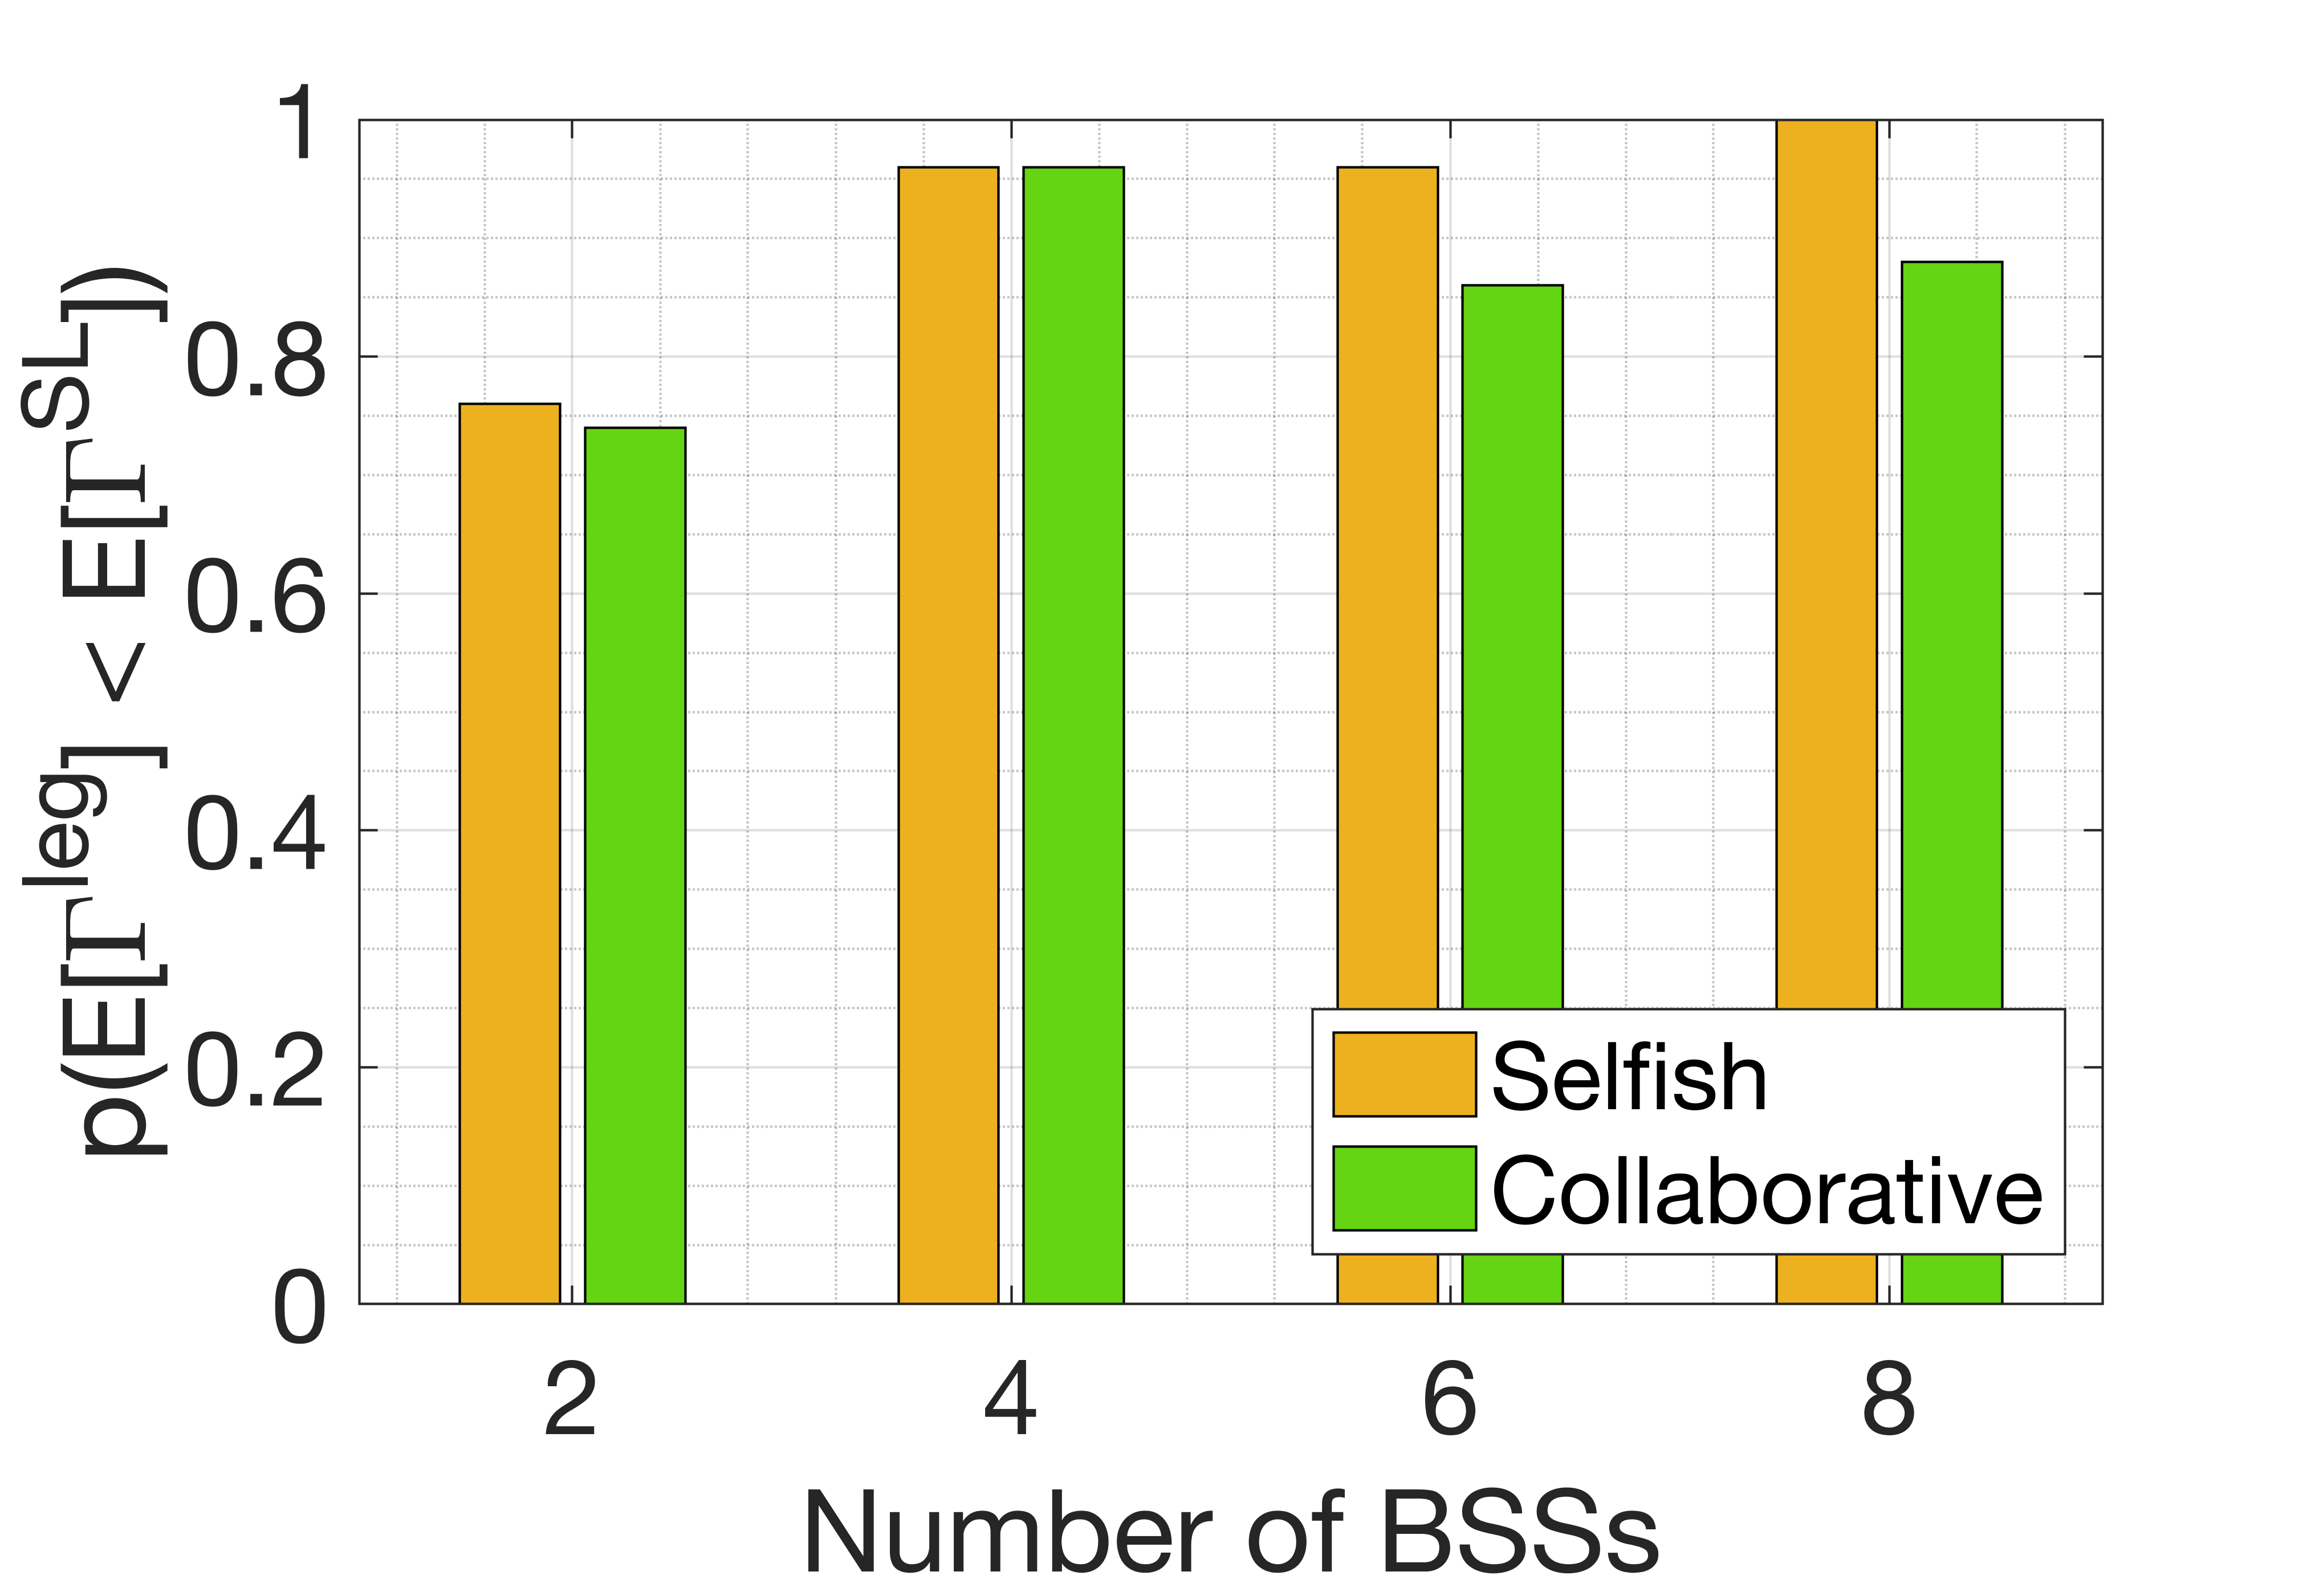
\includegraphics[width=1\textwidth,height=\textheight,keepaspectratio]{img/robustness_average}	
				\end{figure}
			\end{column}
			\hspace{-0.75cm}			
			\begin{column}{4cm}
				\begin{figure}
					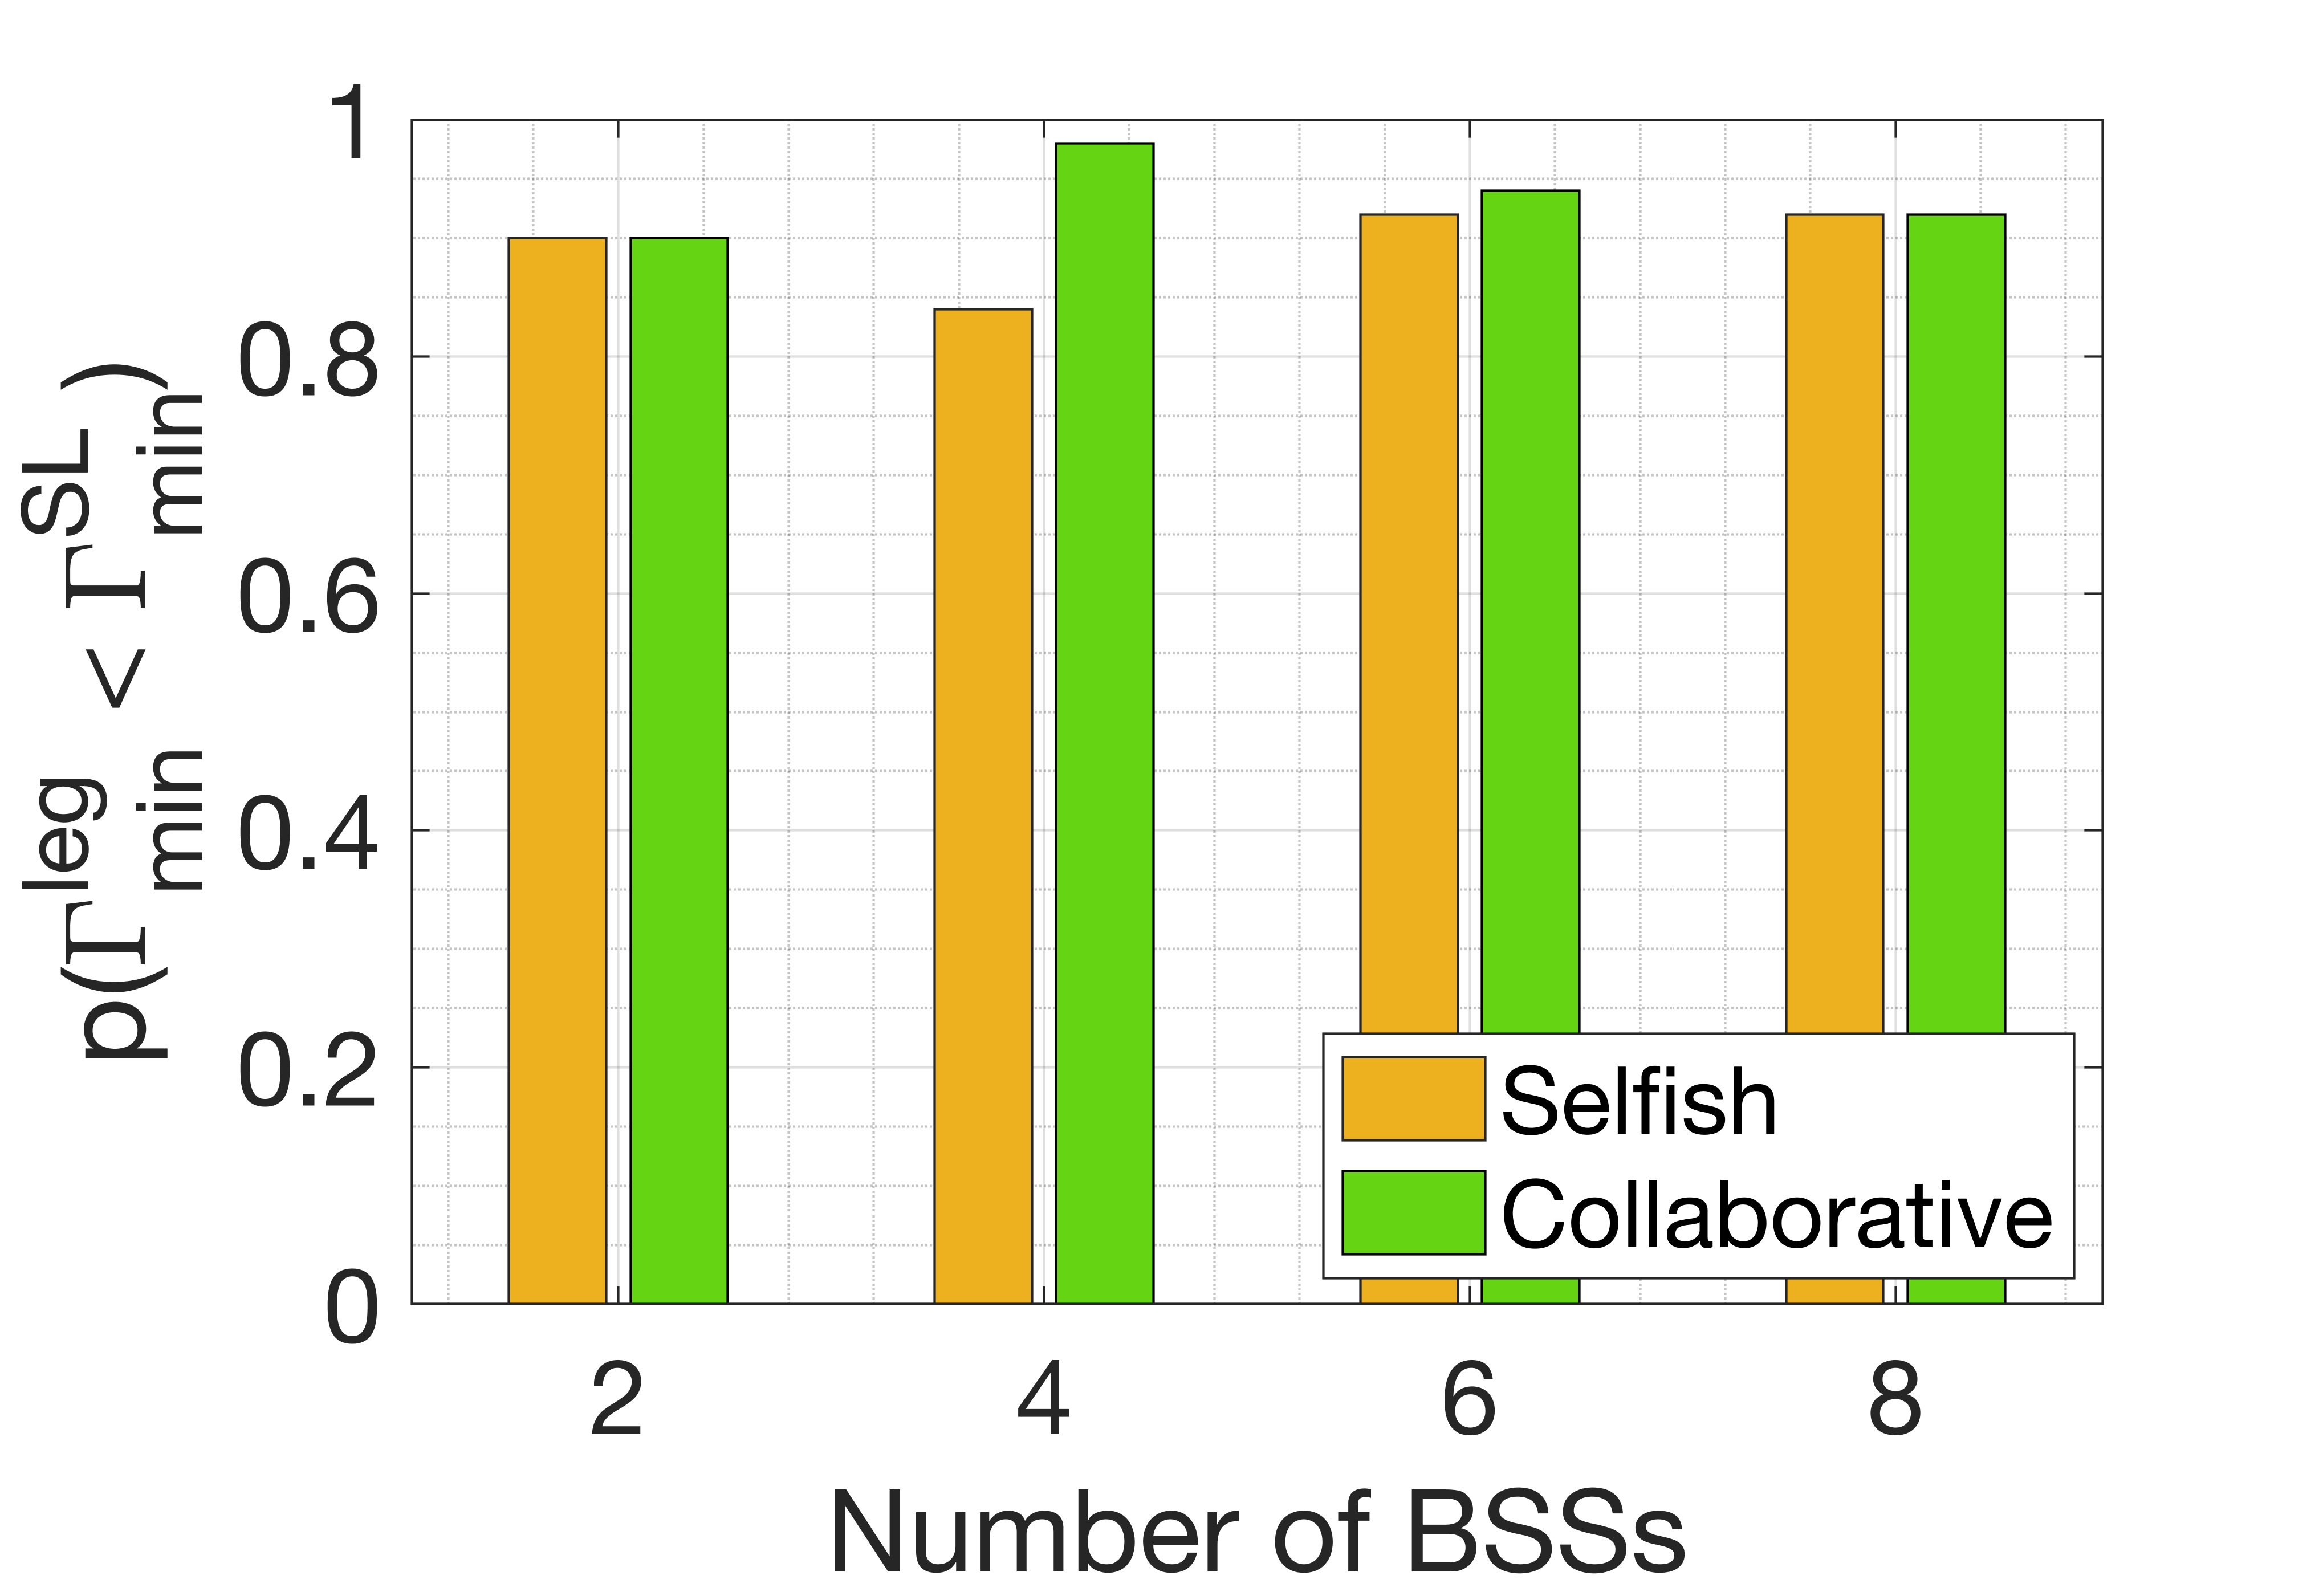
\includegraphics[width=1\textwidth,height=\textheight,keepaspectratio]{img/robustness_maxmin}	
				\end{figure}
			\end{column}
		\end{columns}
	\end{column}
\end{columns}
\end{frame}

%\begin{frame}{Potential and pitfalls of sequentially learned SR}

%\begin{itemize}
%	\only<1>{\item \textbf{Performance improvements}
%	\item \textcolor{gray}{Properties of selfish and cooperative settings}
%	\item \textcolor{gray}{Challenges preventing short-time optimality}}%ocal information, combinatorial action space, complex optimization function, network dynamics}
%	\only<2>{\item \textcolor{gray}{Performance improvements}
%		\item \textbf{Properties of selfish and cooperative settings}
%		\item \textcolor{gray}{Challenges preventing short-time optimality}
%	}
%	\only<3->{\item \textcolor{gray}{Performance improvements}
%		\item \textcolor{gray}{Properties of selfish and cooperative settings}
%		\item \textbf{Challenges preventing short-time optimality}
%	}
%\end{itemize}

%\only<1>{\begin{figure}
%	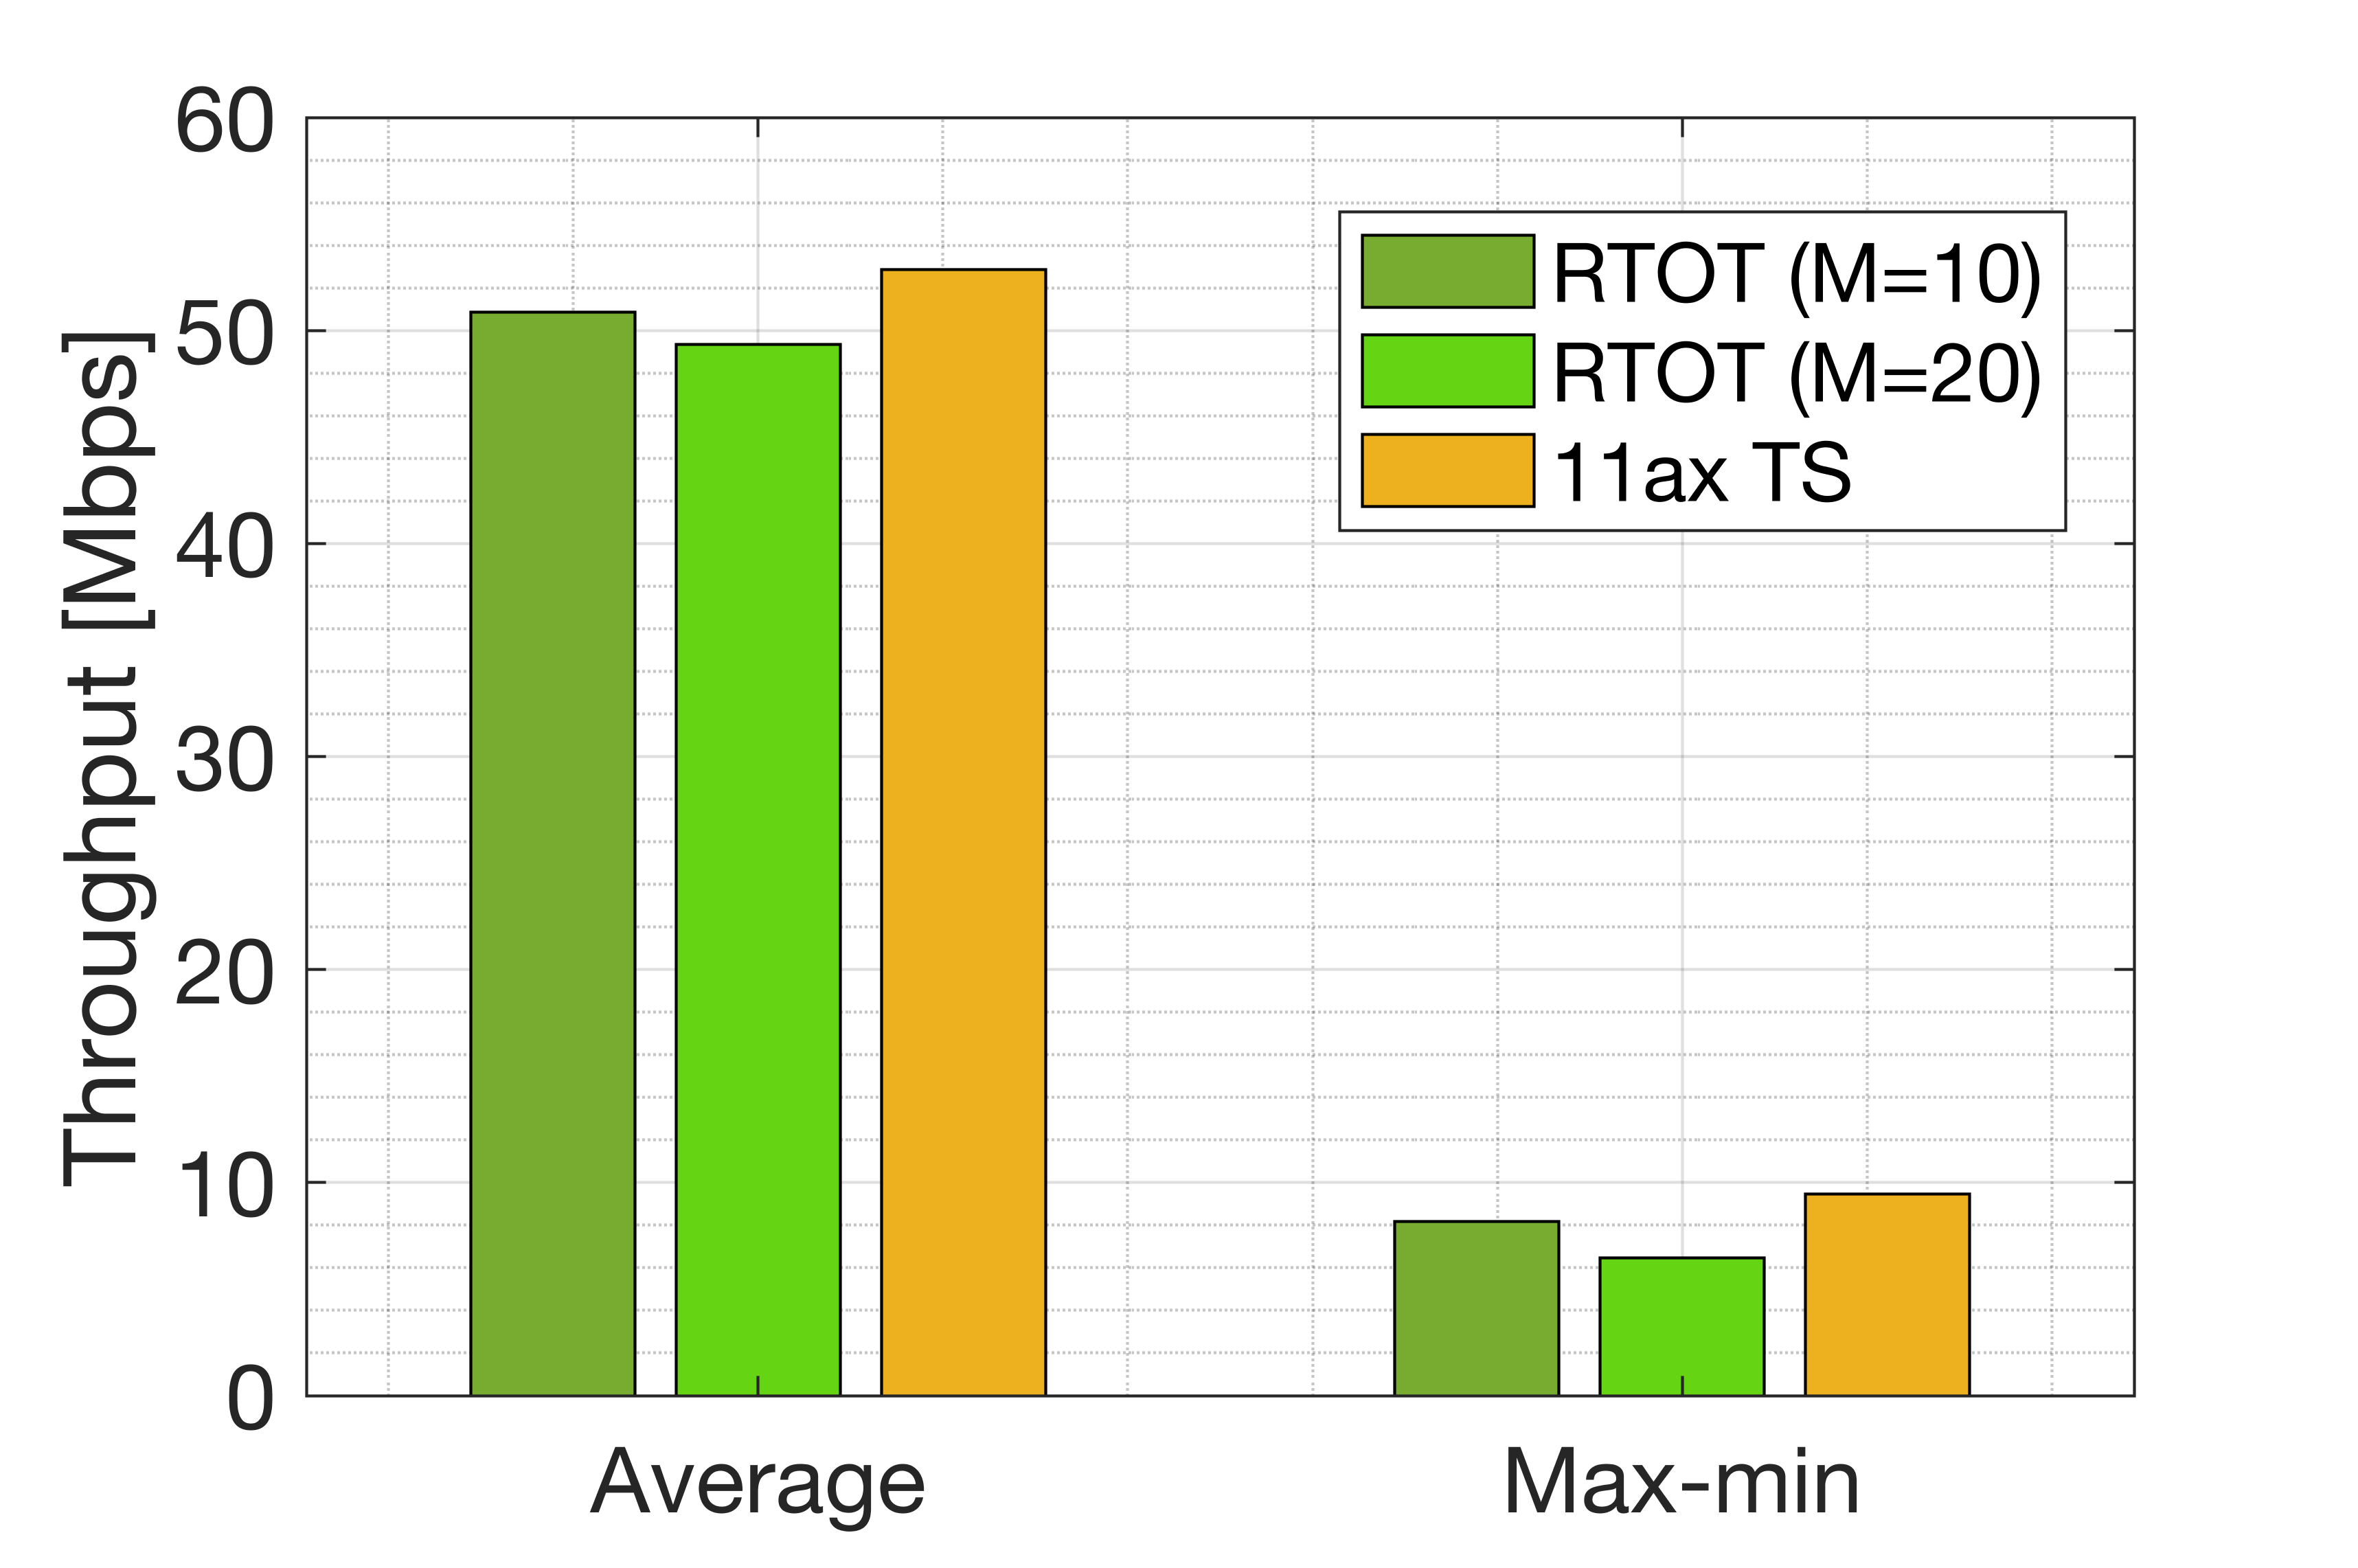
\includegraphics[width=.5\textwidth,height=\textheight,keepaspectratio]{img/output_rtot_vs_learning}
%\end{figure}}

%\only<2>{\begin{columns}\begin{column}{5cm}
%		\begin{figure}
%			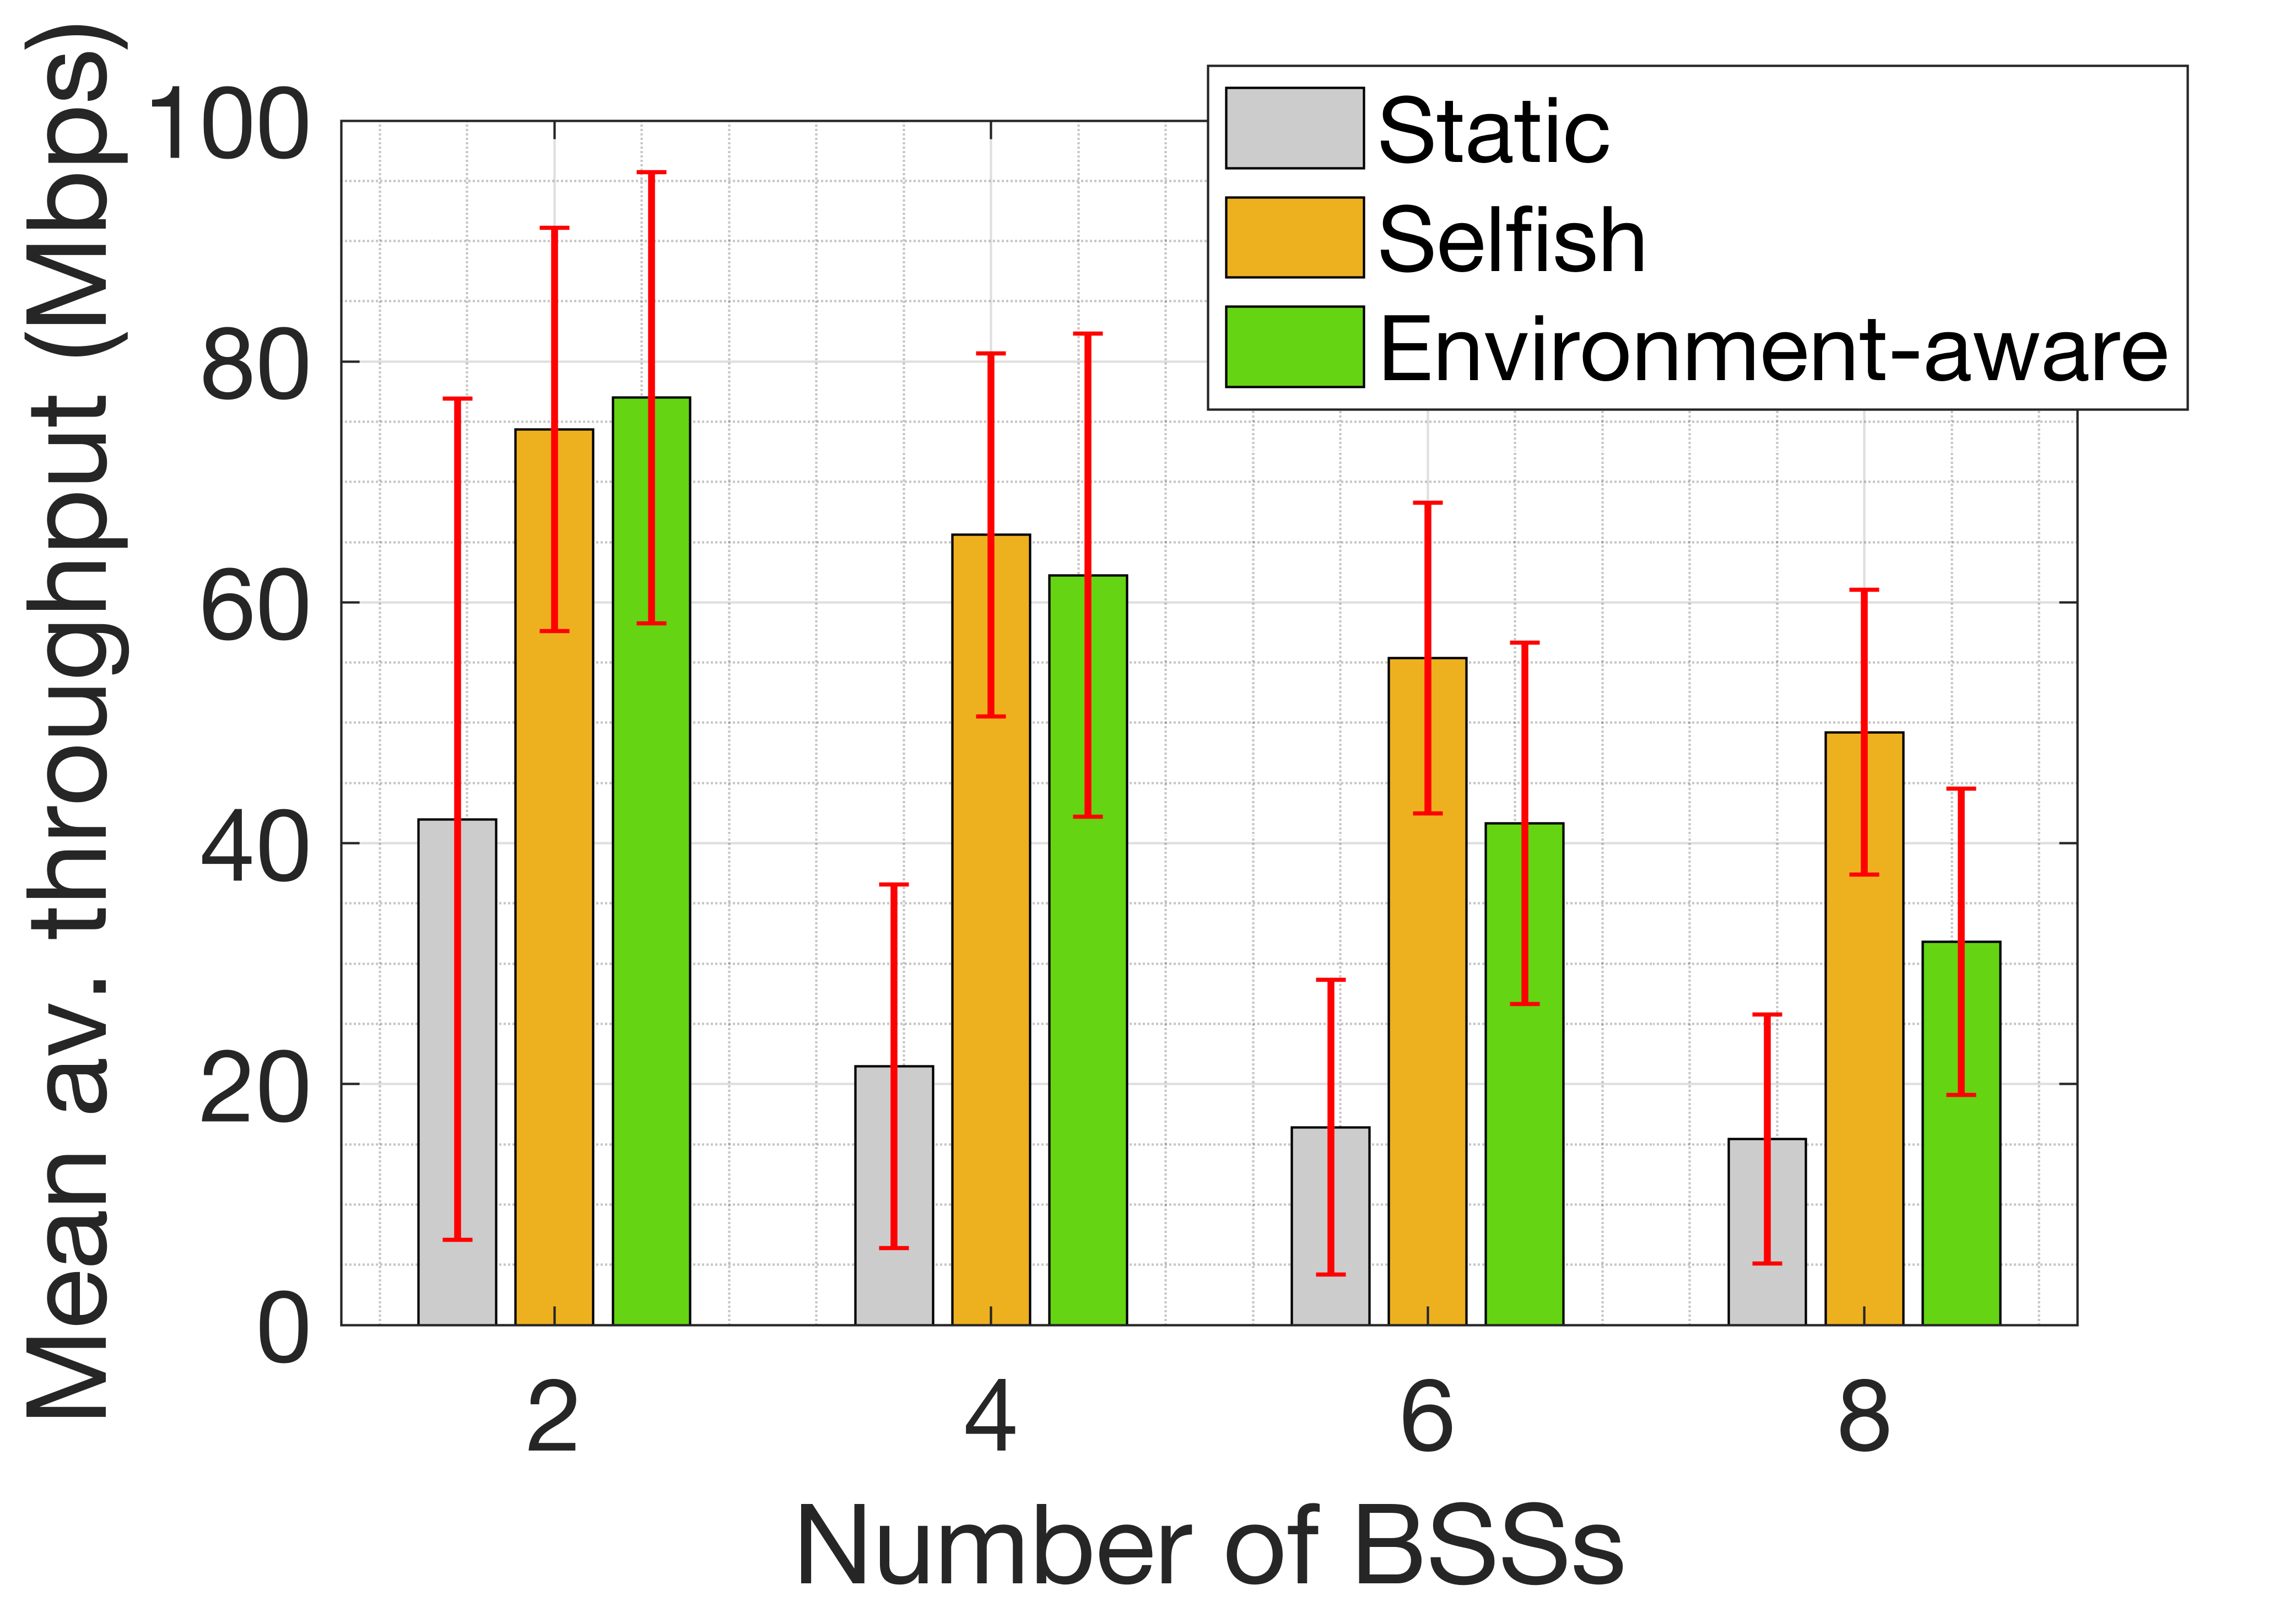
\includegraphics[width=1\textwidth,height=\textheight,keepaspectratio]{img/paper_5_scalability_mean_tpt}
%		\end{figure}
%	\end{column}
%	\begin{column}{5cm}
%		\begin{figure}
%			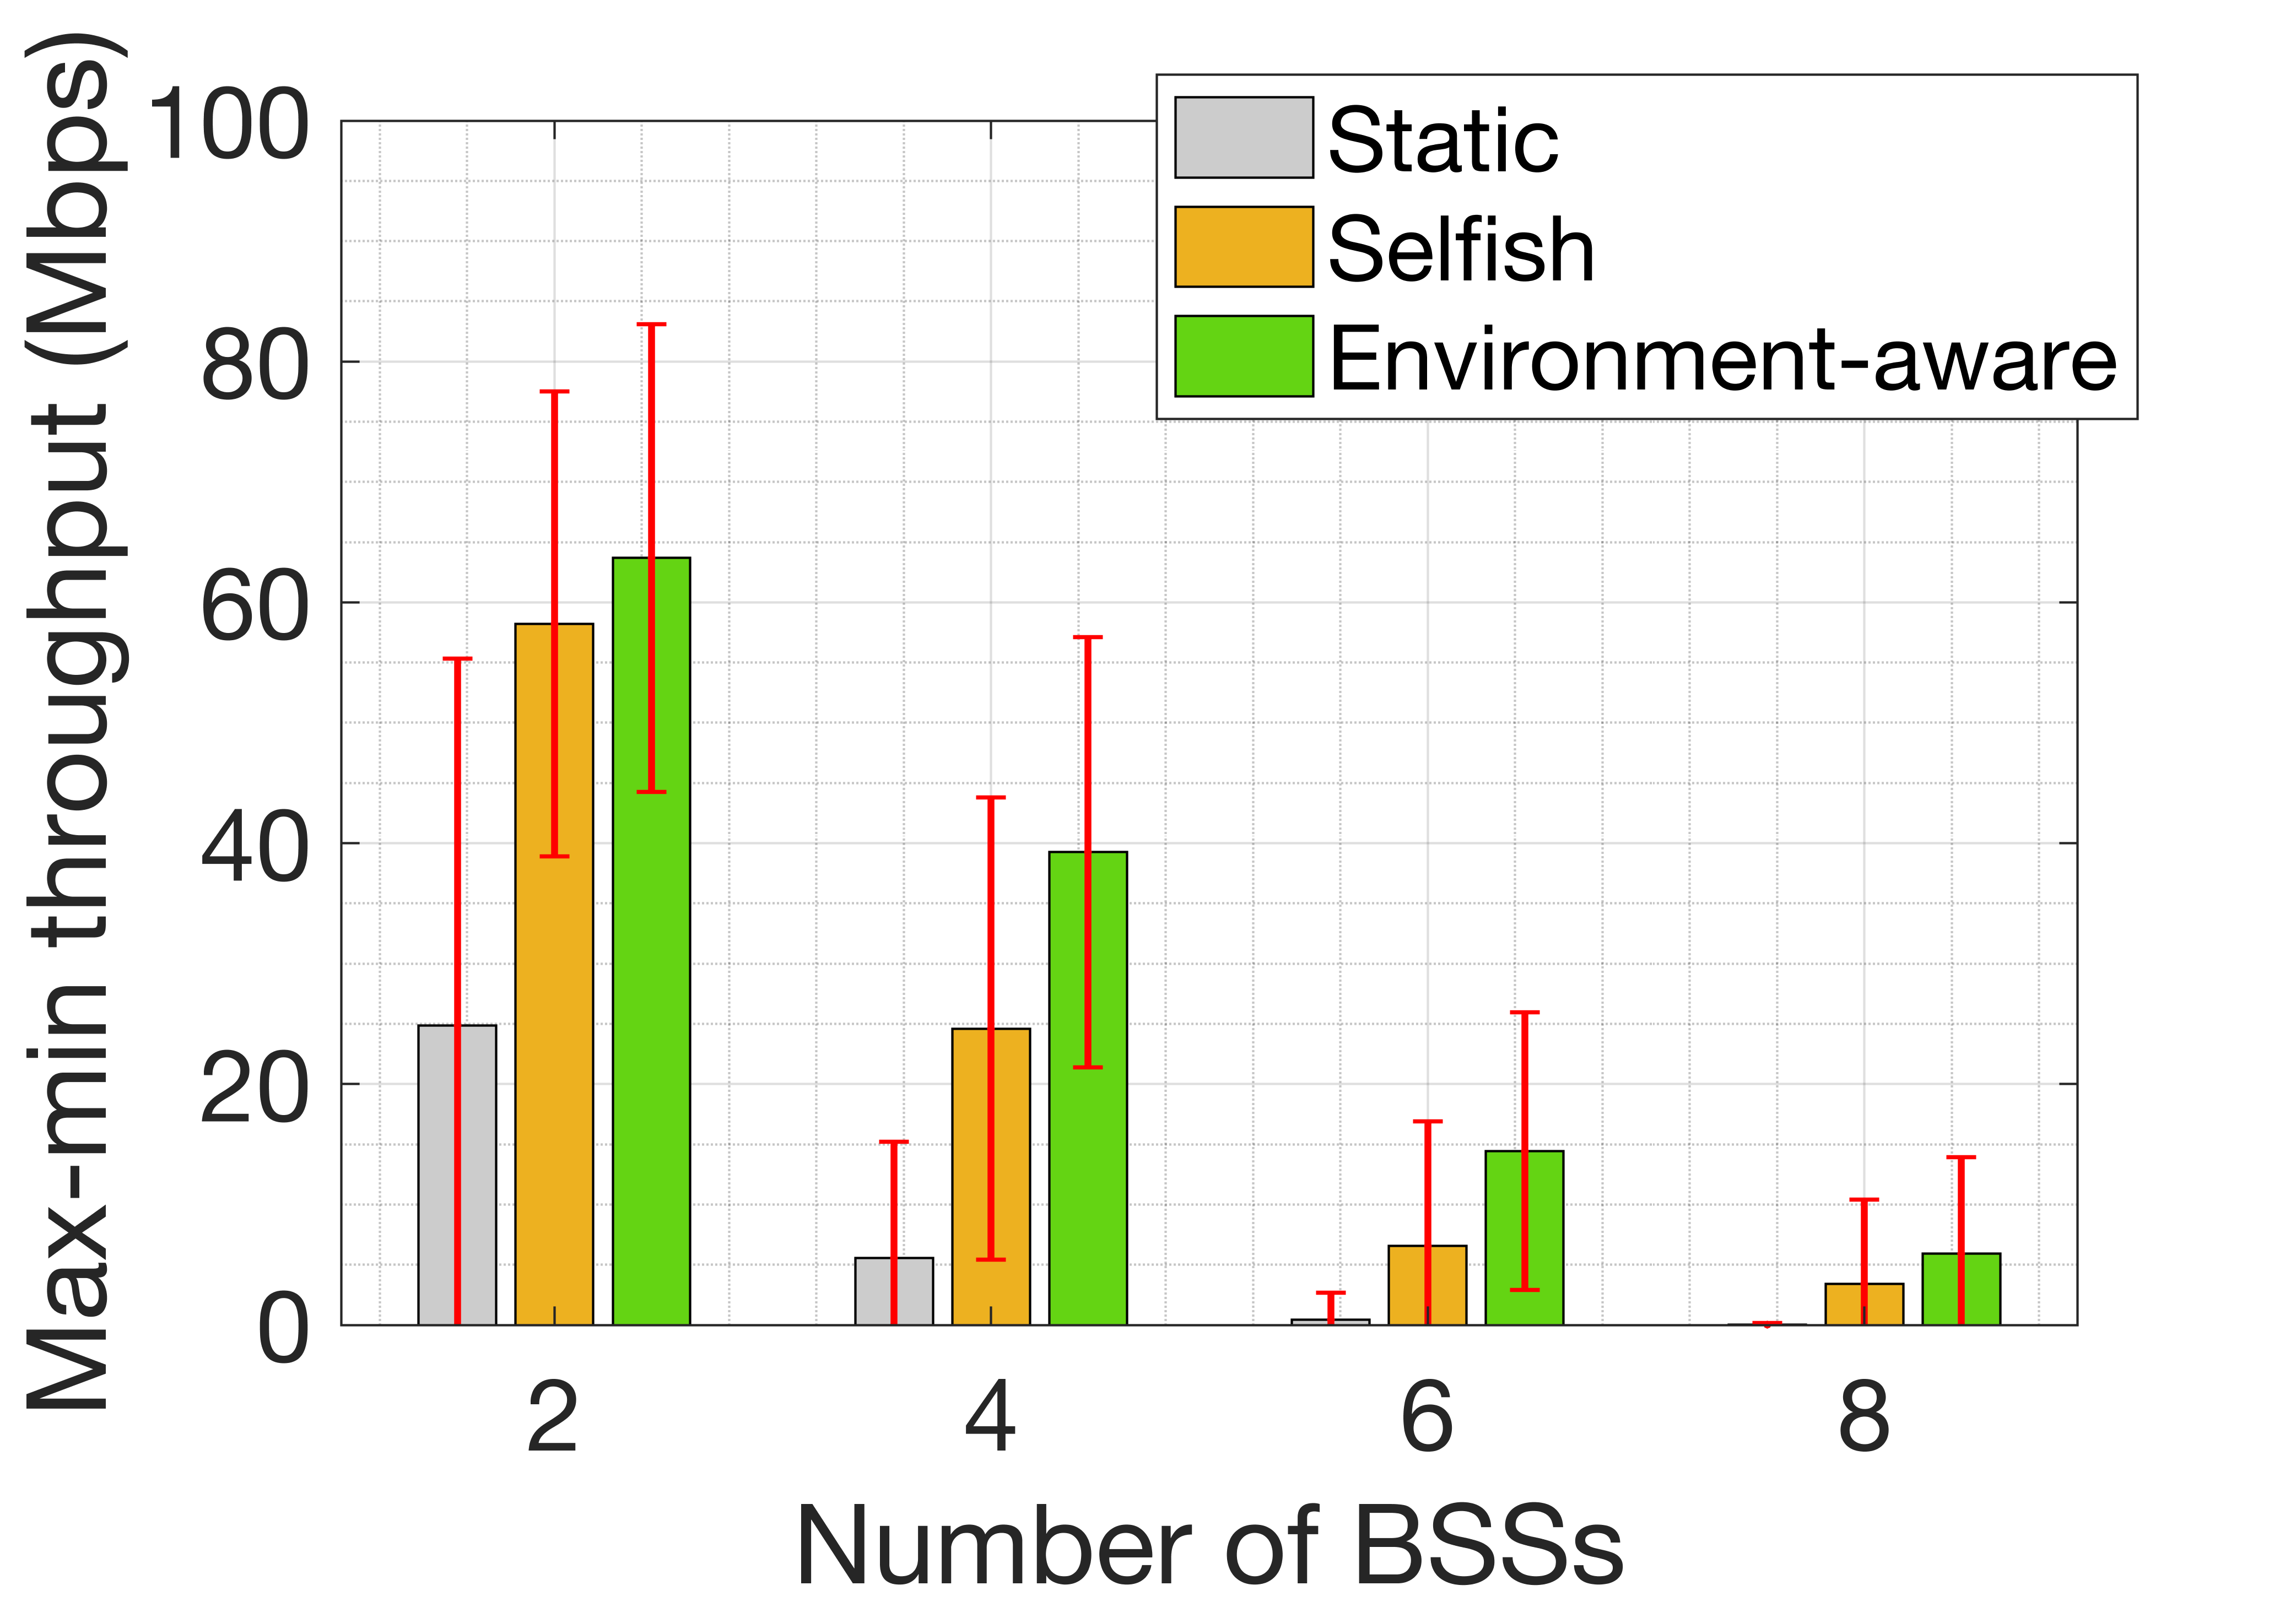
\includegraphics[width=1\textwidth,height=\textheight,keepaspectratio]{img/paper_5_scalability_mean_maxmin}
%		\end{figure}
%	\end{column}
%\end{columns}}
%
%\begin{columns}
%	\begin{column}{6cm}
%		\only<3>{\begin{figure}
%			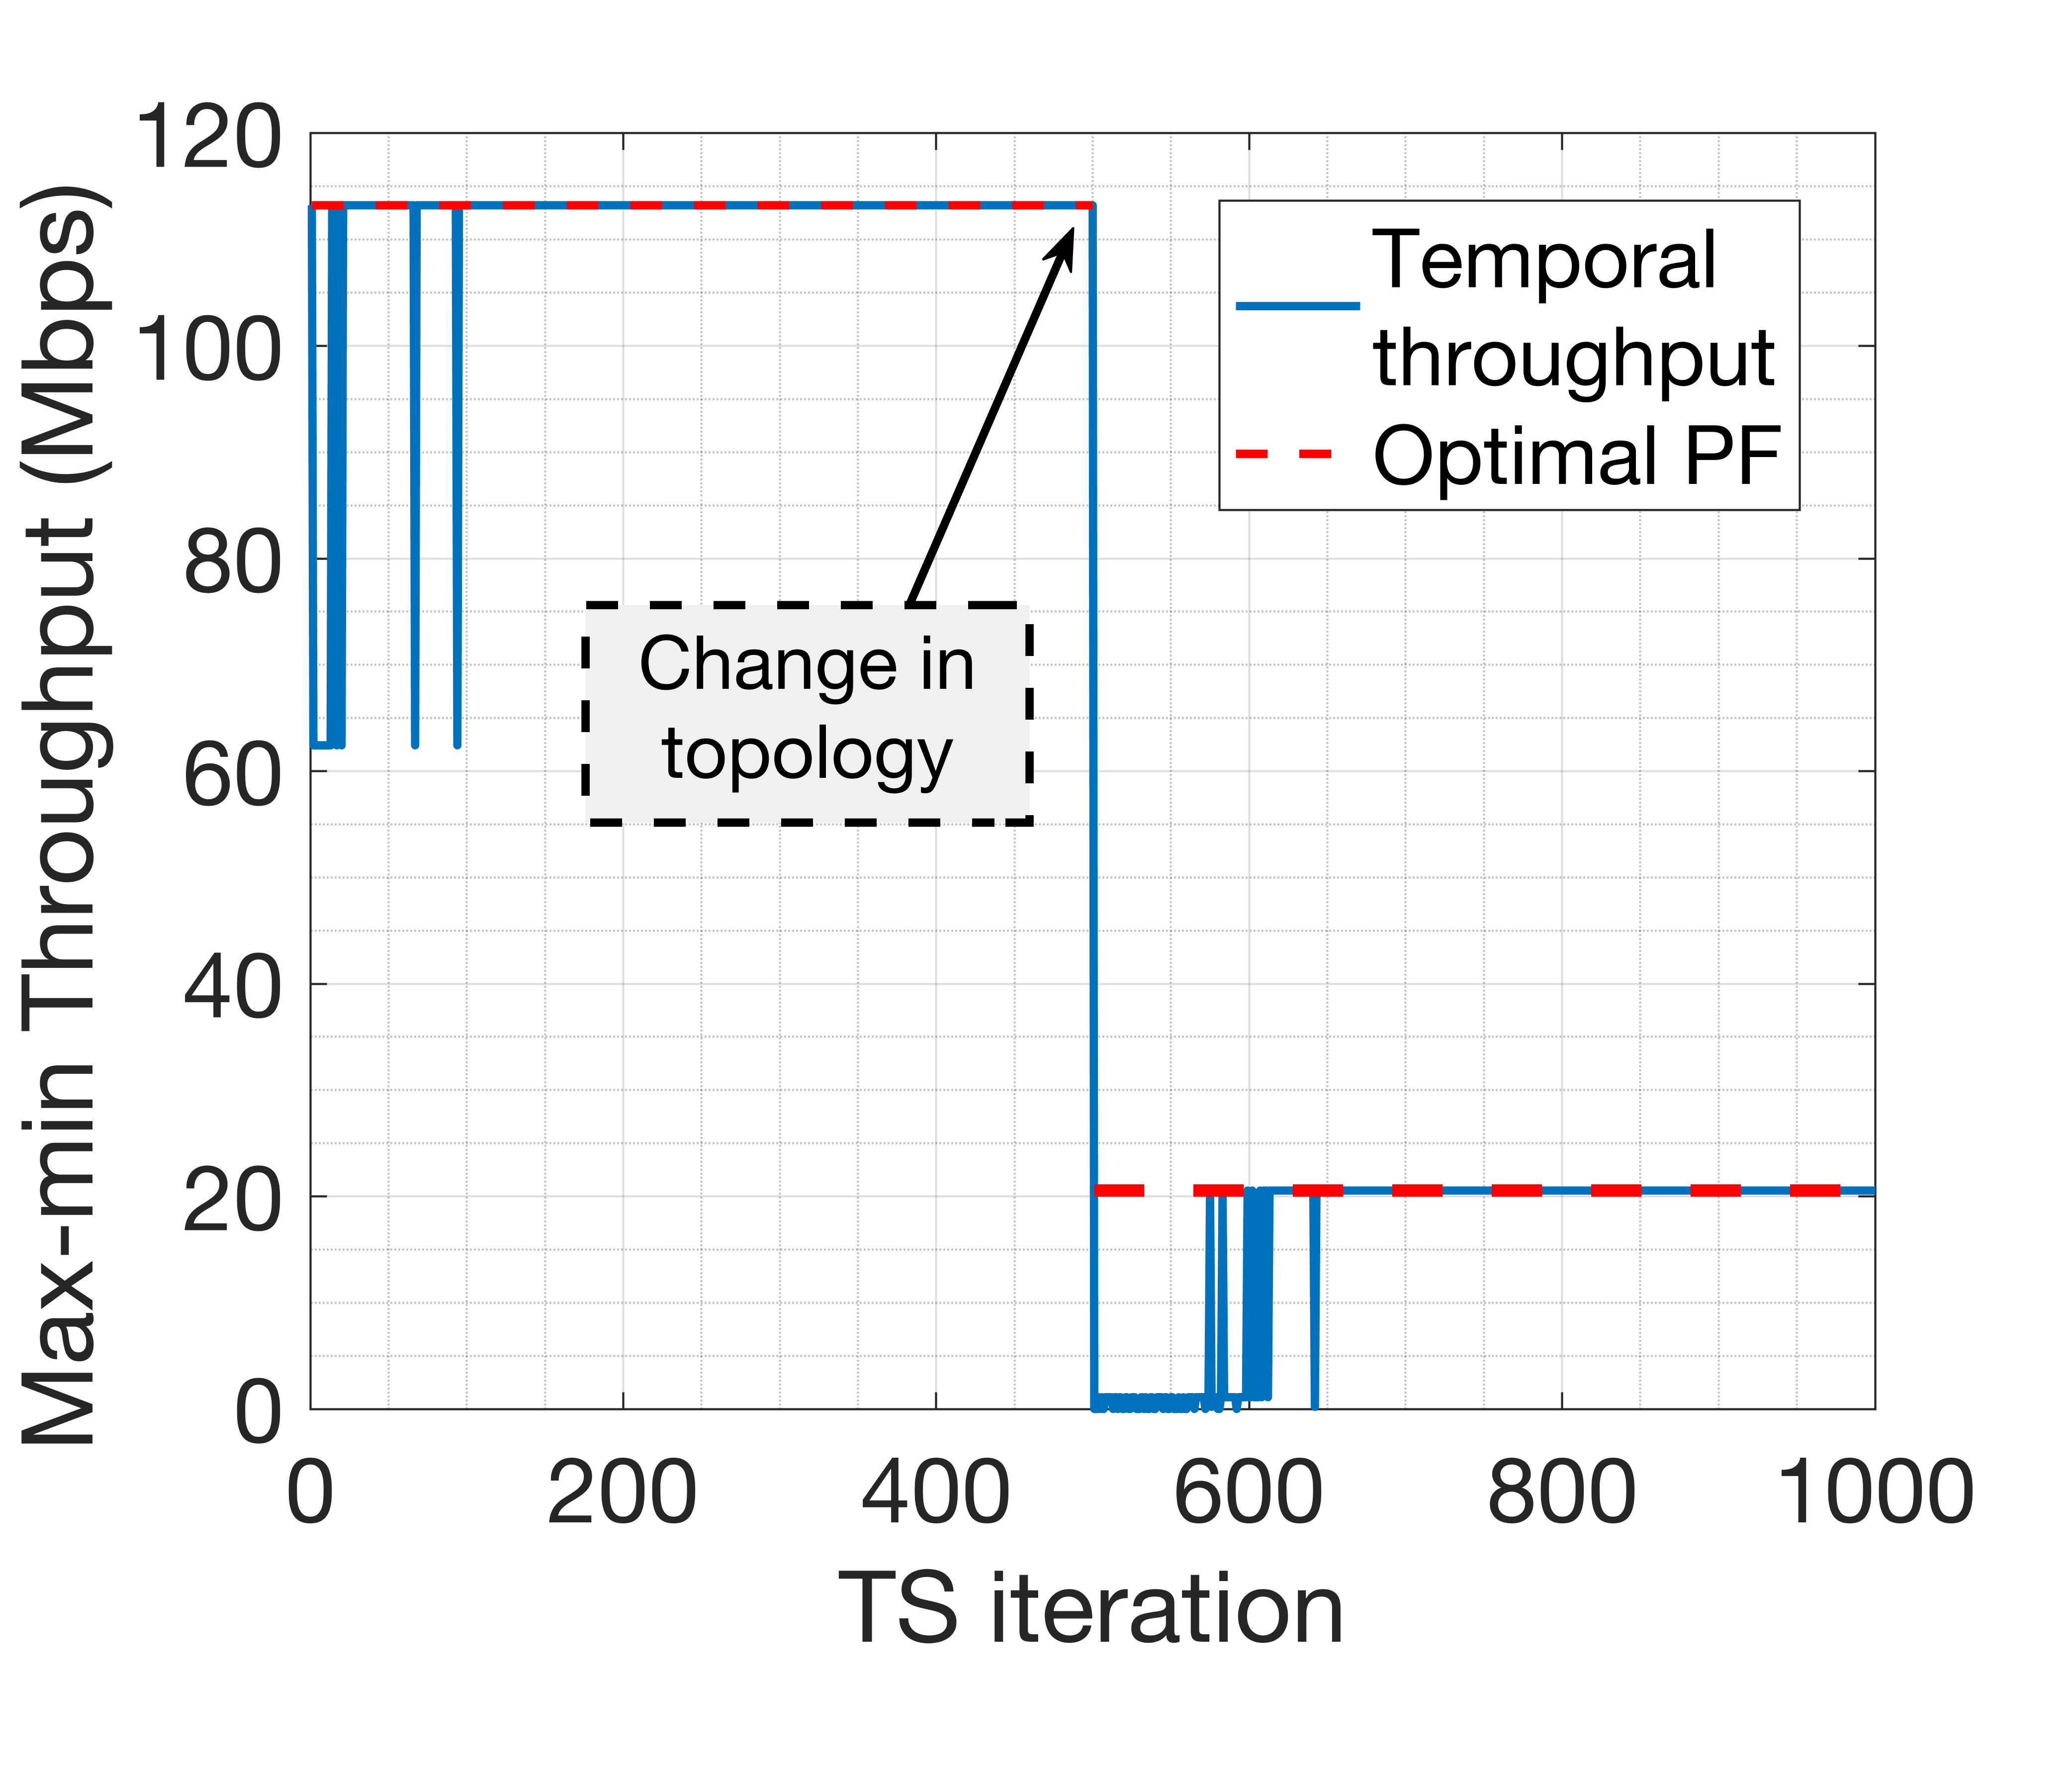
\includegraphics[width=.9\textwidth,height=\textheight,keepaspectratio]{img/paper_5_change_network}
%		\end{figure}}
%		\only<4>{\begin{figure}
%				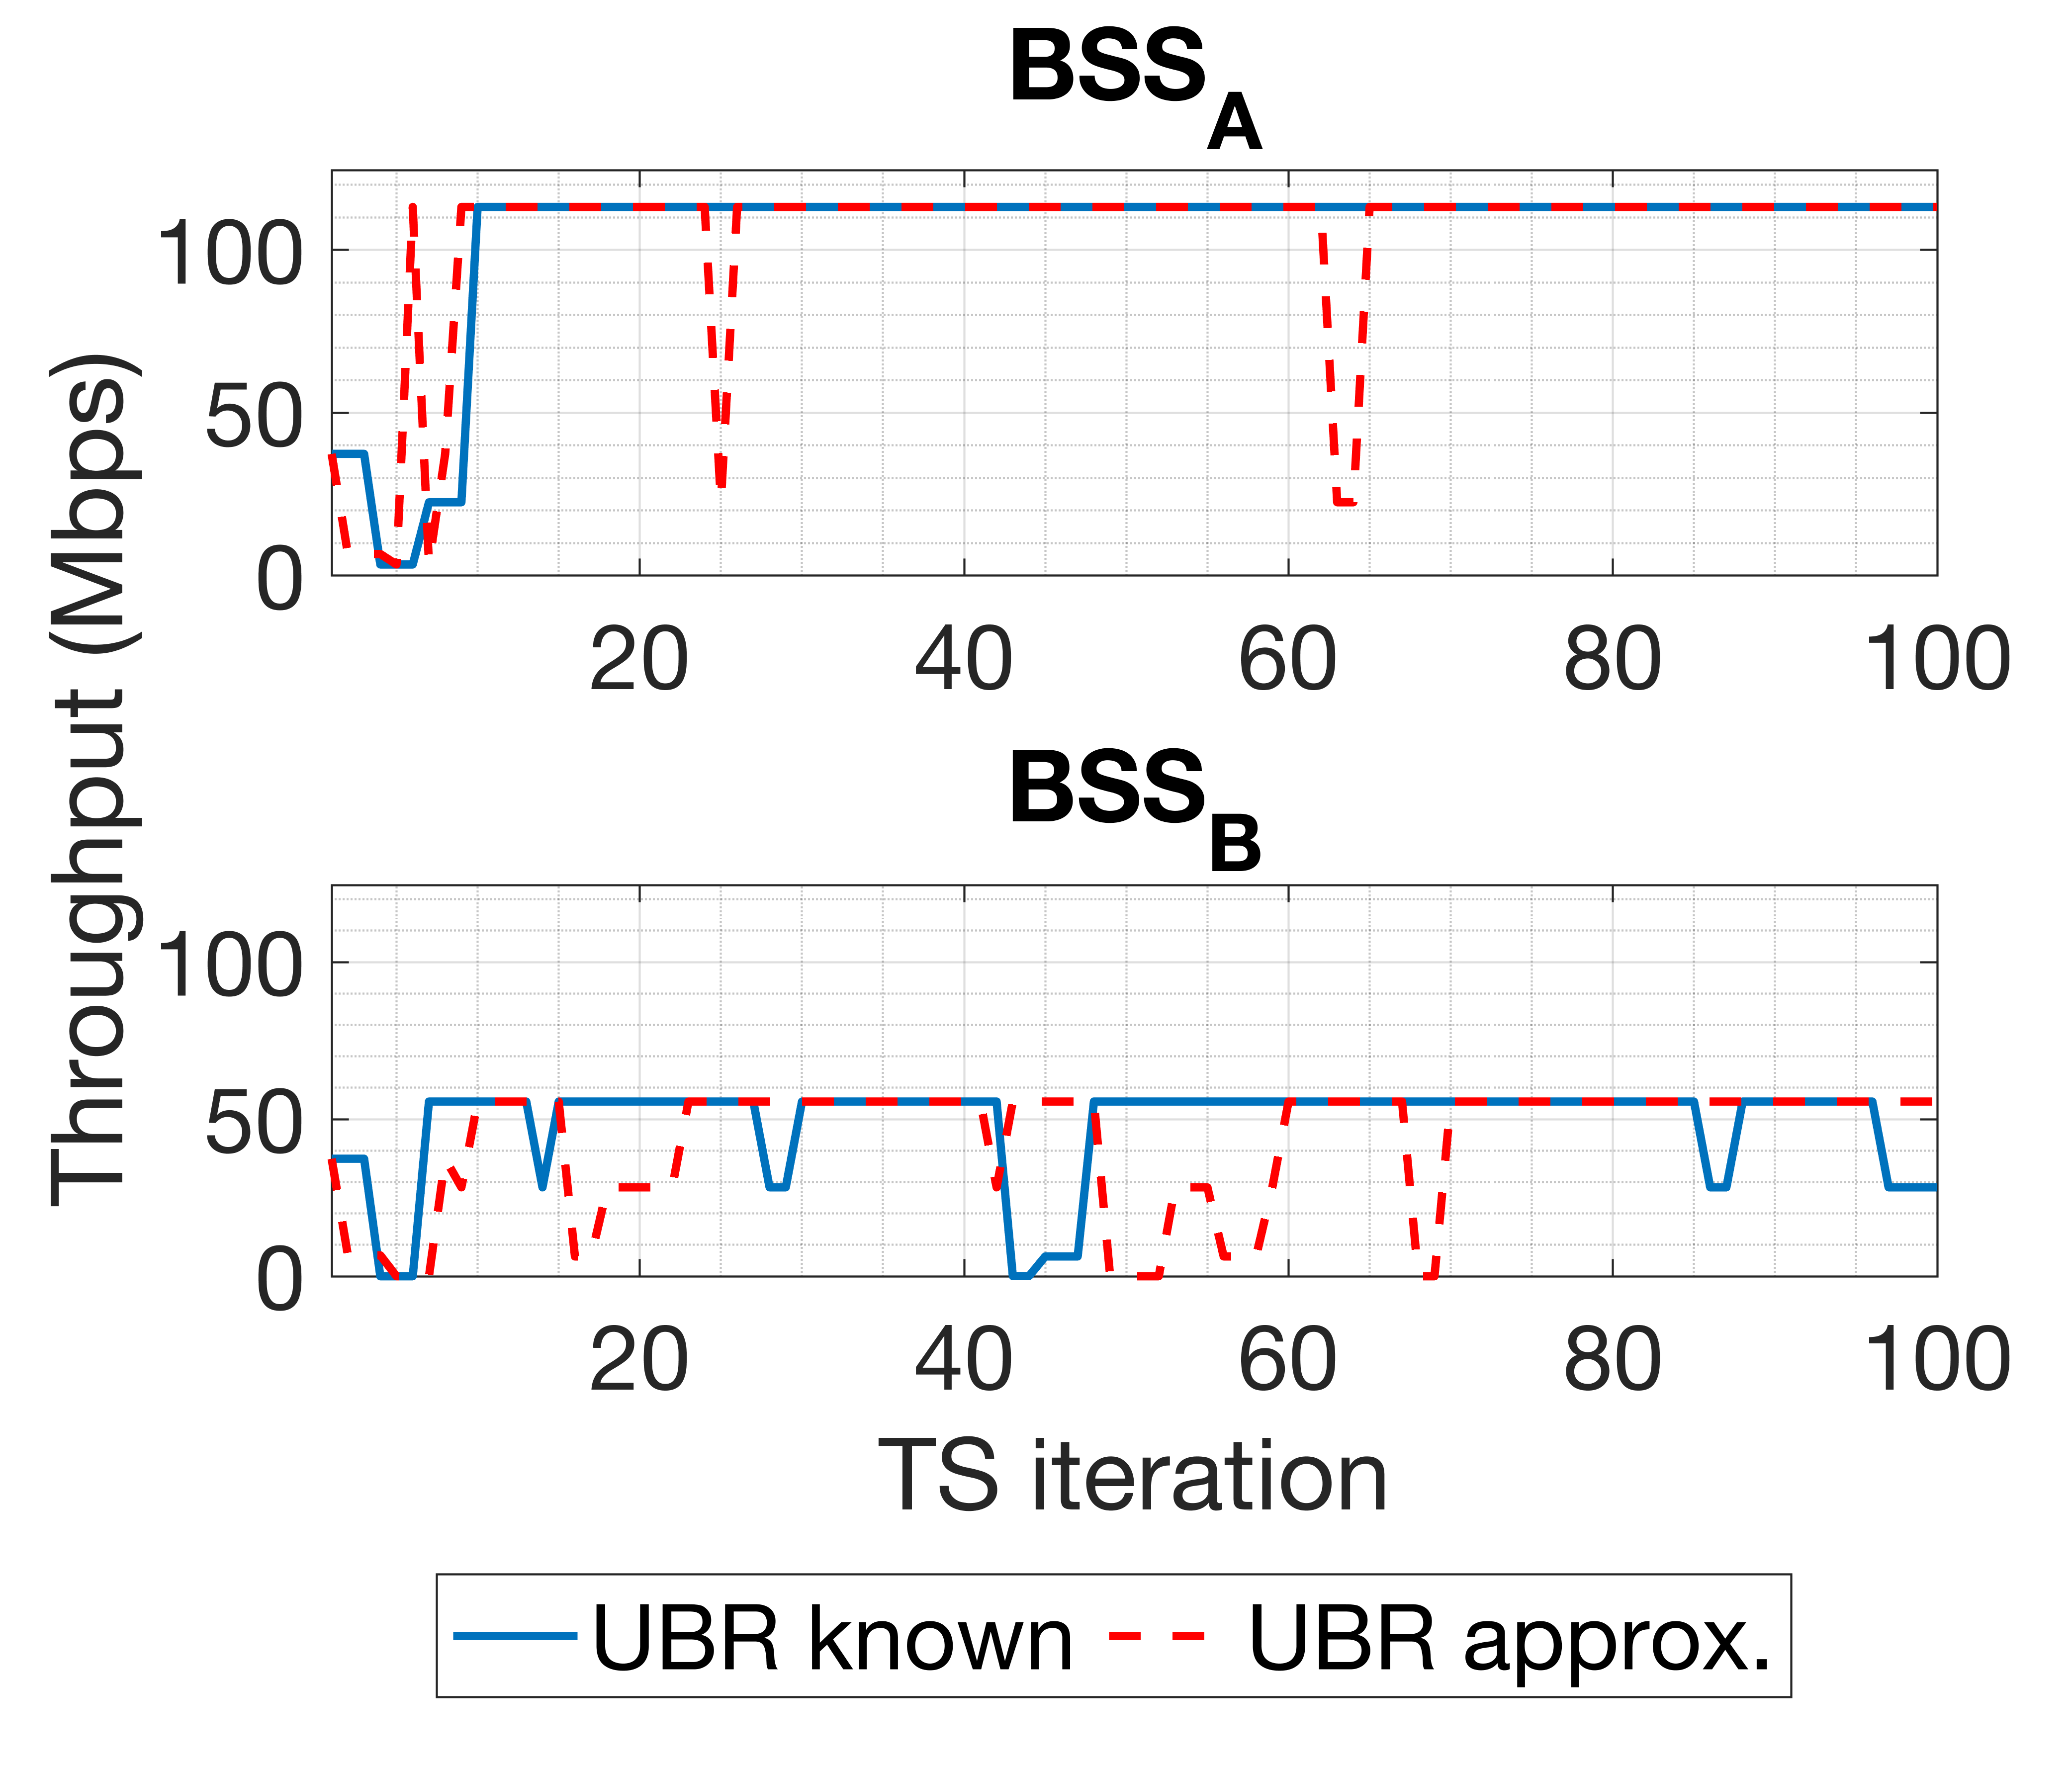
\includegraphics[width=.9\textwidth,height=\textheight,keepaspectratio]{img/paper_5_approx_vs_actual_tpt}
%		\end{figure}}
%		\only<5>{\begin{figure}
%				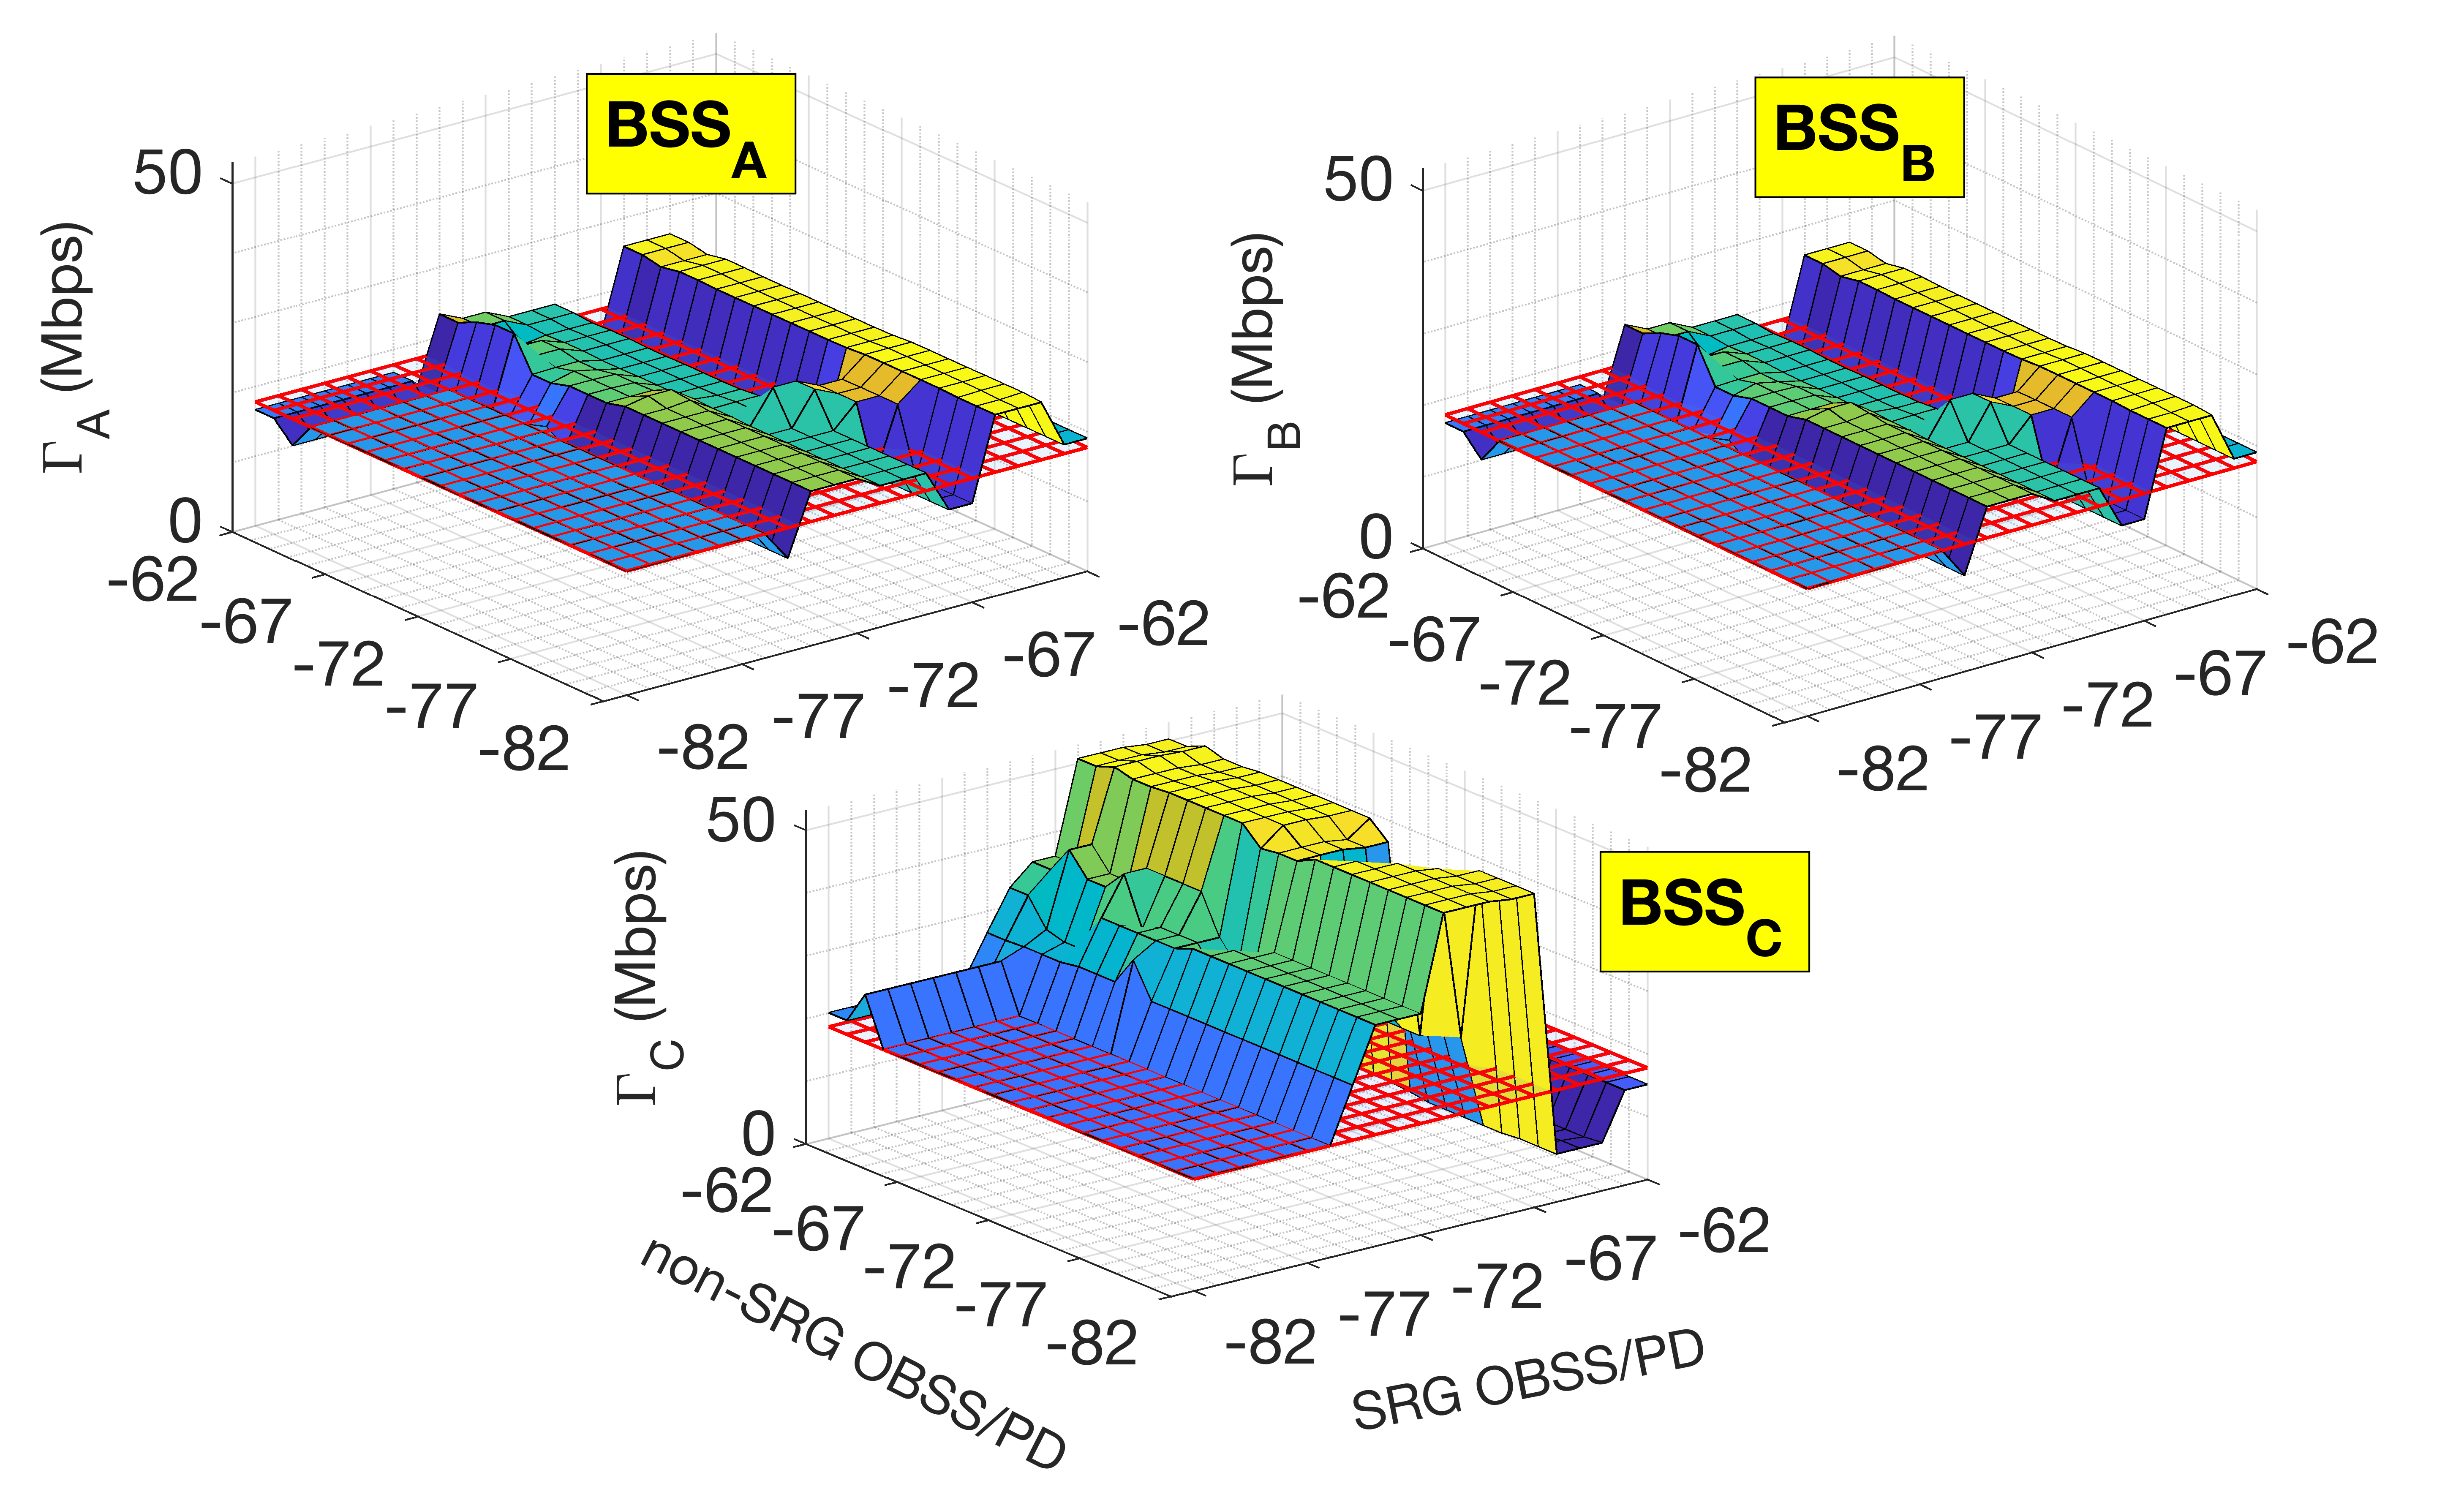
\includegraphics[width=1.1\textwidth,height=\textheight,keepaspectratio]{img/thesis_clashing_interests}
%		\end{figure}}
%	\end{column}
%	\begin{column}{5cm}
%		\only<3->{Some important issues:}
%		\only<3>{\begin{itemize}
%			\item \textbf{Network dynamics}
%			\item \textcolor{gray}{Lack of information}
%			\item \textcolor{gray}{Potential function}
%			\item \textcolor{gray}{...}
%		\end{itemize}}
%		\only<4>{\begin{itemize}
%				\item \textcolor{gray}{Network dynamics}
%				\item \textbf{Lack of information}
%				\item \textcolor{gray}{Potential function}
%				\item \textcolor{gray}{...}
%		\end{itemize}}
%		\only<5>{\begin{itemize}
%				\item \textcolor{gray}{Network dynamics}
%				\item \textcolor{gray}{Lack of information}
%				\item \textbf{Potential function}
%				\item \textcolor{gray}{...}
%		\end{itemize}}
%\end{column}
%\end{columns}
%
%%\begin{alertblock}{}
%%		Promising self-learned solutions but need to improve (trade-off between communication overhead and effectiveness of the solution)
%%\end{alertblock}
%
%%\item \textcolor{gray}{Questions: obsolete data, how much training, complexity of the solution (e.g., states)...}
%
%\end{frame}

%%%%%%%%%%%%%%
%%% Conclusions
%%%%%%%%%%%%%%
\section{Conclusions}

\subsection{}
\begin{frame}{Final remarks}
\pause
\begin{block}{Current status of SR}
	\begin{itemize}
		\item Increasing popularity of SR
		\item Performance limited by current mechanisms
	\end{itemize}
\end{block}
\pause
\begin{exampleblock}{Role of Machine Learning}
	\begin{itemize}
		\item Feasibility of sequential learning to keep decentralization
		\item Need for robust and reliable methods (role of simulators)
	\end{itemize}
\end{exampleblock}
\pause
\begin{alertblock}{Future of SR}
	\begin{itemize}
		\item Evolution of SR towards coordinated settings
		\item AI/ML can enable end-to-end optimization along with other technologies (e.g., OFDMA)
	\end{itemize}
\end{alertblock}

\end{frame}

%%% ACKS
\section{}
\begin{frame}{Funding Sources and Project Acknowledgments}
\begin{scriptsize}
	\begin{itemize}
		\item The Spanish Ministry of Economy and Competitiveness, \textit{Grant number: Maria de Maeztu Units of Excellence program, MDM-2015-0502}
		\item Generalitat de Catalunya, ``Ajuts per donar suport a les activitats dels grups de recerca'', \textit{Grant number: 2017-SGR-11888}
		\item The Spanish Ministry of Science and Innovation, ``Proyectos de I+D de Generación de Conocimiento 2018'', \textit{Grant number: PGC2018-099959-B-I00 (MCIU/AEI/FEDER,UE), WINDMAL (Machine Learning for Wireless Networking in Highly Dynamic Scenarios)}
		\item Cisco University Research Program fund, a corporate advised fund of Silicon Valley Community Foundation, \textit{Grant number: Project CG No. 890107, Towards Deterministic Channel Access in High-Density WLANs}
		\item Santander Universidades, ``Becas Iberoamérica. Santander Investigación'', 2018/19. \textit{Project: Performance Inference in Dense WLANs to Achieve Environment-Aware Learning}.
		\item StandICT.eu, European Commission under the Horizon 2020 Programme, \textit{Short Term (ST) Grant Agreement no. 780439}
	\end{itemize}
\end{scriptsize}
\end{frame}

%%% Questions
\section{}
\begin{frame}{Questions}
\begin{figure}
	
\includegraphics[width=\textwidth,height=0.4\textheight,keepaspectratio]{img/question_mark.png}
\end{figure}

\begin{center}
	\footnotesize
	\textbf{Francesc Wilhelmi}\\
	\textcolor{blue}{francisco.wilhelmi@upf.edu}\\
	Ph.D. Candidate\\
	Department of Communication and Information Technologies\\
	Universitat Pompeu Fabra (Barcelona)
\end{center}

\end{frame}

\appendix



% Backup slides here
\backupbegin
% List of publications
\section{Back-up content}

\begin{frame}{List of publications}
\begin{scriptsize}\begin{enumerate}
		\item Wilhelmi, F., Bellalta, B., Cano, C., \& Jonsson, A. (2017, October). \textit{Implications of decentralized Q-learning resource allocation in wireless networks}. PIMRC.
		\item Wilhelmi, F., Cano, C., Neu, G., Bellalta, B., Jonsson, A., \& Barrachina-Muñoz, S. (2019). \textit{Collaborative spatial reuse in wireless networks via selfish multi-armed bandits.} Ad Hoc Networks.
		\item Wilhelmi Roca, F., Barrachina Muñoz, S., Bellalta, B., Cano, C., Jonsson, A., \& Neu, G. (2019). \textit{Potential and pitfalls of multi-armed bandits for decentralized spatial reuse in WLANs.} Journal of Network and Computer Applications.
		\item Barrachina-Muñoz, S., Wilhelmi, F., Selinis, I., \& Bellalta, B. (2019, April). \textit{Komondor: a wireless network simulator for next-generation high-density WLANs.} Wireless Days.
		\item Wilhelmi, F., Muñoz, S. B., Cano, C., Selinis, I., \& Bellalta, B. (2019). \textit{Spatial Reuse in IEEE 802.11 ax WLANs.} arXiv preprint arXiv:1907.04141.
		\item Wilhelmi, F., Barrachina-Muñoz, S., \& Bellalta, B. (2019, October). \textit{On the Performance of the Spatial Reuse Operation in IEEE 802.11 ax WLANs.} CSCN.
		\item Wilhelmi, F., Barrachina-Munoz, S., Bellalta, B., Cano, C., Jonsson, A., \& Ram, V. (2020). \textit{A Flexible Machine-Learning-Aware Architecture for Future WLANs.} IEEE Communications Magazine.
		\item Wilhelmi, F., Carrascosa, M., Cano, C., Ram, V., \& Bellalta, B. (2020). \textit{Usage of Network Simulators in Machine-Learning-Assisted 5G/6G Networks.} IEEE Wireless Communications Magazine.
\end{enumerate}\end{scriptsize}
\end{frame}

% References 
\begin{frame}[allowframebreaks]{References}
\scriptsize
\bibliographystyle{amsalpha}
\bibliography{bib}
\end{frame}


\backupend

%\begin{frame}{References}
%\tiny
%	\begin{itemize}
%	\citem{1} Smith, G. K. (2017). U.S. Patent No. 9,596,702. Washington, DC: U.S. Patent and Trademark Office.
%	\citem{2} 11-18-1926-02-0eht-terminology-for-ap-coordination
%	\end{itemize}
%\end{frame}

\end{document}